%% LyX 2.0.3 created this file.  For more info, see http://www.lyx.org/.
%DIF LATEXDIFF DIFFERENCE FILE
%DIF DEL diff/diffPreamble.tex   Thu Jun 19 10:43:55 2014
%DIF ADD diff/diffPreamble.tex   Thu Jun 19 10:43:55 2014
%% Do not edit unless you really know what you are doing.
\documentclass[12pt,english]{kuthesis}
\usepackage{mathptmx}
\renewcommand{\sfdefault}{lmss}
\renewcommand{\ttdefault}{lmtt}
\usepackage[T1]{fontenc}
\usepackage[utf8]{inputenc}
\usepackage{listings}
\usepackage{geometry}
\geometry{verbose,tmargin=1in,bmargin=1in,lmargin=1in,rmargin=1in}
\setcounter{secnumdepth}{3}
\setcounter{tocdepth}{3}
\usepackage{url}
\usepackage{graphicx}
\usepackage{wrapfig}
\usepackage{setspace}
\usepackage{esint}
\usepackage{hyperref}
\usepackage{xcolor}
\usepackage{easylist}
\usepackage{multirow}
\usepackage{hhline}
\usepackage{lineno}
%\usepackage{mathtools}
%\usepackage[authoryear]{natbib}

\graphicspath{{IntroductionChapter/figures/},{TheoryChapter/figures/}
  ,{DetectorChapter/figures/},{AnalysisChapter/figures/}
  ,{ResultsChapter/figures/},{ConclusionChapter/figures/}
  ,{FutureWorksChapter/figures/},{ZDCRecoChapter/figures/}
  ,{TriggerChapter/figures/},{SystematicsChapter/figures/}}

\newcommand{\JPsi}{J/$\psi$}
\newcommand{\pt}{$p_{T}$}

\doublespacing

\makeatletter

%%%%%%%%%%%%%%%%%%%%%%%%%%%%%% LyX specific LaTeX commands.
\providecommand{\LyX}{L\kern-.1667em\lower.25em\hbox{Y}\kern-.125emX\@}
%% Because html converters don't know tabularnewline
\providecommand{\tabularnewline}{\\}

%%%%%%%%%%%%%%%%%%%%%%%%%%%%%% User specified LaTeX commands.

%used to align decimals in tables according to APA style
\usepackage{dcolumn}
\usepackage{booktabs}

% Set the title and author info
\title{Ultra-peripheral J/$\psi$ production in PbPb collisions at $\sqrt{s_{NN}}$=2.76 TeV with CMS}
\author{R. Patrick Kenny III}


\dept{Department of People who read Abstracts}
\degreetitle{Doctor of Philosophy}
\papertype{Dissertation} %capitalization is important here
\committee{MEMBER 1}{MEMBER 2}{MEMBER 3}{MEMBER 4}{}

\@printd@testrue
\datedefended{October 02, 2012}
\dateapproved{October 03, 2012}

\@ifundefined{showcaptionsetup}{}{%
 \PassOptionsToPackage{caption=false}{subfig}}
\usepackage{subfig}
\makeatother

\usepackage{babel}
%DIF PREAMBLE EXTENSION ADDED BY LATEXDIFF
%DIF UNDERLINE PREAMBLE %DIF PREAMBLE
\RequirePackage[normalem]{ulem} %DIF PREAMBLE
\RequirePackage{color}\definecolor{RED}{rgb}{1,0,0}\definecolor{BLUE}{rgb}{0,0,1} %DIF PREAMBLE
\providecommand{\DIFaddtex}[1]{{\protect\color{blue}\uwave{#1}}} %DIF PREAMBLE
\providecommand{\DIFdeltex}[1]{{\protect\color{red}\sout{#1}}}                      %DIF PREAMBLE
%DIF SAFE PREAMBLE %DIF PREAMBLE
\providecommand{\DIFaddbegin}{} %DIF PREAMBLE
\providecommand{\DIFaddend}{} %DIF PREAMBLE
\providecommand{\DIFdelbegin}{} %DIF PREAMBLE
\providecommand{\DIFdelend}{} %DIF PREAMBLE
%DIF FLOATSAFE PREAMBLE %DIF PREAMBLE
\providecommand{\DIFaddFL}[1]{\DIFadd{#1}} %DIF PREAMBLE
\providecommand{\DIFdelFL}[1]{\DIFdel{#1}} %DIF PREAMBLE
\providecommand{\DIFaddbeginFL}{} %DIF PREAMBLE
\providecommand{\DIFaddendFL}{} %DIF PREAMBLE
\providecommand{\DIFdelbeginFL}{} %DIF PREAMBLE
\providecommand{\DIFdelendFL}{} %DIF PREAMBLE
%DIF END PREAMBLE EXTENSION ADDED BY LATEXDIFF
%DIF PREAMBLE EXTENSION ADDED BY LATEXDIFF
%DIF HYPERREF PREAMBLE %DIF PREAMBLE
\providecommand{\DIFadd}[1]{\texorpdfstring{\DIFaddtex{#1}}{#1}} %DIF PREAMBLE
\providecommand{\DIFdel}[1]{\texorpdfstring{\DIFdeltex{#1}}{}} %DIF PREAMBLE
%DIF END PREAMBLE EXTENSION ADDED BY LATEXDIFF

\begin{document}
  \linenumbers
  \chapter{Introduction}
  \DIFaddbegin \DIFadd{High energy physics probes the smallest scales in order to discover the 
    fundamental constituents of the universe and how they interact.
  From these searches of the smallest scales, the standard model of particle
    physics has emerged. 
  The standard model contains 3 forces, the weak, the electromagnetic, and 
    strong force, and two types of mater that interact through these forces,
    quarks and leptons.
  The quarks can interact through all three forces.
  The leptons however only interact through the weak and electromagnetic force.
  The mater particles interact with each through the three forces by exchanging the
    forces carrying vector bosons. 
  Strong interactions take place by exchange of gluons, the weak by Z$^{0}$ and
    W$^{\pm}$ bosons, and the electromagnetic by photon. 
  }

  \DIFadd{Each of these three forces emerges due to symmetries in the standard model.
  For example, the wave function of the Sch}\"{o}\DIFadd{rdinger equation is comprised
    of complex numbers.
  The standard model does not depend on the phase of these complex numbers. 
  The phases for each of these numbers can be arbitrarily changed at all points
    in space and time without any changing the predictions of the theory.
  This is because the gradient of an arbitrary scaler field can be added to the
    $\vec{A}$, the vector potential, which gives rise to the electromagnetic 
    without changing the magnetic field and electric field that ultimately
    interact with the particles. 
  The invariance of the standard model to the complex phase of the wave 
    function necessitates the existence of the electromagnetic force. 
}

  \DIFadd{The standard model is made of the three such symmetries, each of which is
    described by a gauge group. 
  The U(1) is the group that accounts for the electromagnetic interaction
    and gives rise to the photon. 
  The SU(2) group produces the weak bosons, Z$^{0}$ and W$^{\pm}$.
  The strong force mediated by the gluons are consequence of the SU(3) symmetry
    of the standard model.
  Of these three groups two, SU(2) and SU(3), are non-abelian. 
  The consequence of this, is that the W$^{+}$ and W$^{-}$ can interact with 
    Z$^{0}$ and photon, the gluons can interact with each other. 
  Because the gluons can interact with each other in many more ways that the 
    limited interactions between the W,Z and the photons, the non-abelian 
    nature of the strong force is particularly pronounced. 
}

  \DIFadd{The self-interaction of the gluons produces unique qualities of the strong 
    force: confinement, and asymptotic freedom. 
  }

  \DIFadd{Microseconds after the big bang, the universe existed in a state known as
    the Quark Gluon Plasma (QGP).
  In the QGP, quarks and gluons are not in hadronic bondage, forced to 
    the confines of bound states such as protons and neutrons.
  The Large Hadron Collider (LHC) produces QGP in the lab in PbPb (lead-lead)
    collisions.
  The high energies and rates of the collisions at the LHC make it possible 
    to do detailed studies of the QGP. 
  The LHC is producing rare experimental probes such as suppressed jets and 
    heavy quarkonia at an unprecedented rate in heavy-ion collisions. 
  Physicists now have better constraints on the properties like temperature,
    viscosity, and energy density of the QGP. 
  }\DIFaddend \section{Theoretical Context}
  \section{History }

  \chapter{Photo-nuclear interactions \label{ch:photoNuc}}
    In ultra-peripheral heavy-ion collision, the colliding nuclei interact only 
      electromagnetically~\cite{Baltz:2007kq,Bertulani:2005ru}.   
    In such events, no QGP state emerges, and the effects arising from the QGP 
      no longer obscure the initial state effects.
    Other initial state probes such as peripheral nuclear collisions and 
      proton-nucleus collisions have the potential to create the QGP obscuring 
      effects that come from the initial state.
    Hadronic interactions do \DIFdelbegin \DIFdel{no }\DIFdelend \DIFaddbegin \DIFadd{not }\DIFaddend occur in ultra-peripheral collisions (UPC), 
      therefore final state effects coming from the QGP are not expected. 
    Thus, UPC events provide clarity by enhancing \DIFdelbegin \DIFdel{physicists' 
      }\DIFdelend \DIFaddbegin \DIFadd{the }\DIFaddend understanding of the 
      initial state. 

    In particular, these interactions between the field of photons surrounding 
      the colliding nuclei and the gluons within the nuclei can produce a 
      \JPsi{}, probing the gluon density~\cite{Ryskin:1992ui,Brodsky:1994kf}.
    The \JPsi{} can be produced either coherently or incoherently. 
    In the case of coherent interactions, the photon couples to the nucleus 
      as a whole.
    In the incoherent case, the photon couples to the nucleons within the 
      nucleus.
    The UPC \JPsi{} photoproduction cross section is therefore a probe of 
      the initial state of the nucleus.

    This cross section can be calculated using three steps.   
    First, the Weizs\"{a}cker-Williams approximation~\cite{vonWeizsacker:1934sx,Williams:1934ad} provides a way to calculate the 
      density of probing photons that surrounds the nucleus. 
    Second, the electron-proton scattering data gives a value for the proton 
      photoproduction cross section at lower energies \cite{Klasen:2007pm}.
    Last, a specific model is used to combined the previous two steps in order
      to calculate the nuclear photoproduction cross section. 
    In this thesis the Adeluyi and Bertulani (AB)~\cite{pQCD2011.08,pQCD2013.02}, STARlight~\cite{vmd1999,starlight}, and 
      the Leading Twist (LTA)~\cite{Frankfurt:2011cs,lta2011.09} models are discussed. 
    Each of these methods handle the gluon density of the nucleus differently 
      producing a measurable difference in the value of the \JPsi{} 
      photoproduction cross section. 
    There are other UPC models available~\cite{Goncalves:2011vf,Cisek:2012yt,Lappi:2013am,Hufner:1996jw}, 
      but this thesis focuses on the STARlight, the AB, and the LTA models.
    The analysis presented in Chapter~\ref{ch:analysis} adds to the existing 
      data in a new kinematic region.
    In this Chapter, the theoretical framework for photon-nuclear
      interactions, together with an experimental review of recent results on 
      ultra-peripheral heavy-ion collisions are described. 

  \section{Weizs\"{a}cker-Williams approximation \label{sec:wwAprox}}
    The density of photons surrounding the colliding nuclei can be calculated 
      using the Weizs\"{a}cker-Williams approximation~\cite{vonWeizsacker:1934sx,Williams:1934ad}. 
    This approximation relates the electric field of a stationary point charge 
      to the photon field that arises at ultra relativistic velocities. 
    The approximation is semi-classical. 
    In the Weizs\"{a}cker-Williams approximation, a Fourier transform of Maxwell's 
      equations is combined with the quantum mechanical equation for the energy of the photon.   
    \begin{figure}[!Hhbt]
      \begin{center}
        \includegraphics[width=.65\textwidth]{boost.png}
      \end{center}
      \caption{ \label{fig:boost} The electromagnetic field boosted (right) and 
        at rest (left) \cite{WWJackson}.}
    \end{figure}
    The frequency modes of the electrostatic field are treated as photons. 
    The Weizs\"{a}cker-Williams approximation makes the calculation of 
      electromagnetic interactions with the nucleus tractable. 

    The Weizs\"{a}cker-Williams approximation begins with the equation for the 
      electric field of the projectile nucleus at rest. 
    To calculate the photon flux on the target nucleus, the electromagnetic field 
      only needs to be considered at the position of the target nucleus. 
    From the projectile's point of view, the target is moving and contributes
     $-vt$ to Eq.~\ref{eq:staticEFromTargtmp}, the equation for the electric 
     field of the projectile nucleus at rest.
    \begin{equation} \label{eq:staticEFromTargtmp}
        x'=-vt'\textrm{,}\qquad
        y'=b\textrm{,}\qquad
        z'=0\textrm{,}\qquad
        \vec{\mathbf{E'}}=\left(\frac{eZ}
         {4 \pi \epsilon_{0}\left(\left(-vt'\right)^{2}+b^{2}\right)^{3/2}}\right)
         \left(-vt'{\mathbf{\hat{x'}}+b\mathbf{\hat{y'}}}\right)\textrm{,}
    \end{equation}        
      where $b$ is the impact parameter
      defined as the distance of separation at closest approach, $v$ is the velocity of the 
      projectile nucleus, $Z$ is the number of protons in the nucleus, and $e$ 
      is the charge of the electron.
    Two simplifications occur due to the choice of coordinates in 
      Eq.~\ref{eq:staticEFromTargtmp}.
    The magnetic field is equal to zero, as the projectile is at rest, and
      the $z$ coordinate can be ignored, reducing the equation to two dimensions. 

    The Lorentz transformation converts the field equations in the 
      projectile's frame to equations in the target's frame.
    Eq.~\ref{eq:staticEFromTarg2tmp} gives the result of the transformation 
      from the projectile's primed frame to the target's rest frame for 
      the field components \cite{WWJackson}:
    \begin{eqnarray} \label{eq:staticEFromTarg2tmp}
        E_{x}'=E_{x}\textrm{,}\qquad
        \gamma\left(E_{y}'/c+\beta B_{z}'\right)=E_{y}/c\textrm{,}\qquad
        \gamma\left(E_{z}'/c=\beta B_{y}'\right)=E_{z}/c\textrm{,} \nonumber \\
        B_{x}'=B_{x}\textrm{,}\qquad
        \gamma\left(B_{y}'-\beta E_{z}'/c\right)=B_{y}\textrm{, and}\qquad
        \gamma\left(B_{z}'+\beta E_{y}'/c\right)=B_{z}\textrm{.}
    \end{eqnarray}
    The transformation equations for the fields, 
      Eq.~\ref{eq:staticEFromTarg2tmp}, and the transformation of the 
      coordinates reduce to Eq.~\ref{eq:staticEFromTarg3tmp} \cite{WWJackson}:
    \begin{eqnarray} \label{eq:staticEFromTarg3tmp}
        E_{x}'=E_{x}\textrm{,}\qquad
        \gamma E_{y}'=E_{y}\textrm{,}\qquad
        \gamma \beta E_{y}'/c=B_{z}\textrm{,}\nonumber \\
        ct'=\gamma ct\textrm{, and}\qquad
        x'=-\gamma \beta c t\textrm{.}
    \end{eqnarray}
    The Lorentz transformation reduces the six components of the 
      electromagnetic field in the target's frame to the three equations in 
      Eq.~\ref{eq:staticEFromTarg2tmp} by relating them to the fields in the 
      projectile's frame. 

    By combining Eq.~\ref{eq:staticEFromTargtmp} and 
      Eq.~\ref{eq:staticEFromTarg2tmp}, equations for the electric and 
      magnetic fields in the target's rest frame are obtained 
        \begin{eqnarray} \label{eq:ebPframe} 
          \vec{\mathbf{E}}=\left( \frac{\gamma e Z}
           { 4 \pi \epsilon_{0} \left( \left( \gamma v t \right)^{2} 
           + b^{2}\right)^{3/2} }\right)
           \left(vt\mathbf{\hat{x}}+b\mathbf{\hat{y}}\right)\nonumber\textrm{, and} \\
           \vec{\mathbf{B}}=\frac{\gamma\beta e Z b}
           { 4 \pi c \epsilon_{0} \left( \left( \gamma v t \right)^{2} 
           + b^{2}\right)^{3/2} }
           \mathbf{\hat{z}}=
           \frac{\gamma\mu_{0}veZb}{4\pi\left(\left(\gamma v t \right)^{2}
           +b^{2}\right)^{3/2}}\mathbf{\hat{z}}.
        \end{eqnarray}
    If the impact parameter $b$ goes to zero, the target sits in the line of 
      the projectile particle's motion, and the denominator carries a factor of
      $\gamma$ squared. 
    When $vt$ goes to zero, the projectile particle position lays on the 
      $y$-axis, and the numerator carries a factor of $\gamma$. 
    This results in fields that are a factor of $\gamma^3$ higher in the 
      $y$ direction than in the $x$ direction (see Fig.~\ref{fig:boost}).  
    The boost compresses the electric field of the charge 
      in the direction of the boost and produces a magnetic field 
      resulting in a form similar to radiation.
    The point charge at ultra relativistic velocities produces a strong 
      electric field in the plane transverse to its motion resembling a plane 
      wave.

    Separating the electromagnetic field into even and odd functions of time 
      simplifies the decomposition of the field equations into Fourier frequency 
      modes.
    The even functions decompose into cosine functions, odd functions 
      into sine functions. 
    The $y$-component of the electric field and the $z$-component of 
      the magnetic field are even functions in time, and the 
      $x$-component of the electric field is an odd function in time.
    Eq.~\ref{eq:fourier1tmp} gives the Fourier transformation integrals. 
    \begin{eqnarray} \label{eq:fourier1tmp}
        E_{x}(\omega)=\sqrt{\frac{2}{\pi}}\frac{eZ}{4\pi\epsilon_{0}b^{2}}
         \int^{\infty}_{0}\frac{\left(\gamma vt/b\right)\sin
         \left(\omega t\right)}
         {\left(\left(\gamma vt/b\right)^{2}+1\right)^{3/2}}dt\textrm{,} \nonumber\\
          E_{y}(\omega)=\sqrt{\frac{2}{\pi}}\frac{\gamma eZ}
         {4\pi\epsilon_{0}b^{2}} \int^{\infty}_{0}\frac{\cos(\omega t)}
         {\left(\left(\gamma vt/b\right)^{2}+1\right)^{3/2}}dt\textrm{,  and}\\
          B_{z}(\omega)=\frac{\beta E_{y}(\omega)}{c}.\nonumber
    \end{eqnarray}
    The solutions to the integrals of Eq.~\ref{eq:fourier1tmp} are the following
      \cite{WWFermi}:
    \begin{eqnarray}  \label{eq:fourier2tmp}
      u=\frac{\gamma v t}{b}\textrm{,}\qquad du\left(\frac{b}{\gamma v}\right)=dt\textrm{,}\qquad
      \omega'=\frac{\omega b}{\gamma v}\textrm{,}\nonumber \\
      \int^{\infty}_{0}\frac{u \sin(\omega'u)}{\left(u^{2}+1\right)^{3/2}}du
      =\omega'K_{0}(\omega')\textrm{, and}\qquad
      \int^{\infty}_{0}\frac{\cos(\omega'u)}{\left(u^{2}+1\right)^{3/2}}
      =\omega'K_{1}(\omega').
    \end{eqnarray}
    In Eq.~\ref{eq:fourier2tmp}, $\omega$ can be related to the energy of a 
      photon by $E=\hbar\omega$.
    The components of the electric field in terms of $\omega$ are:
    \begin{equation} \label{eq:fourier3tmp}
        E_{x}(\omega)=\sqrt{\frac{2}{\pi}}\frac{eZ}{4\pi\epsilon_{0}b^{2}}
     \frac{b}{\gamma v}\frac{\omega b}{\gamma v}K_{0}
     \left(\frac{\omega b}{\gamma v}\right)\textrm{, and}\qquad
      E_{y}(\omega)=\sqrt{\frac{2}{\pi}}\frac{\gamma eZ}{4\pi\epsilon_{0}b^{2}}
     \frac{b}{\gamma v}\frac{\omega b}{\gamma v}K_{1}
     \left(\frac{\omega b}{\gamma v}\right).\qquad
    \end{equation}
    The $y$-component of the electric field does not have a factor of $t$ in 
      the numerator in Eq.~\ref{eq:fourier1tmp}, therefore the factor of $\gamma$ 
      remains outside of the integral for the Bessel functions in 
      Eq.~\ref{eq:fourier3tmp}.
    In Eq.~\ref{eq:fourier3tmp}, $E_{y}$ carries an additional factor of 
      $\gamma$ in the numerator relative to the $E_{x}$, therefore in the case
      when $\gamma >> 1$, $E_{x}$ can be neglected. 

    When $v$ approaches $c$, $\beta \approx 1$, the $y$-component of the 
      electric field and the $z$-component of the magnetic field are related by 
      a factor of $c$, $E_{y}/c=B_{z}$.
    $E_{y}$ is approximately equally to $\gamma$ $E_{x}$ because $K_{0}(x)$ is 
      smaller than $K_{1}(x)$ for all $x$. 
    The conditions imposed by the ultra-relativistic limit result in the 
      following relationship
    \begin{equation} \label{eq:ultraRelAprox}
      \gamma \gg 1 \Rightarrow \gamma E_{x} \gg E_{x} \Rightarrow E_{y} \gg E_{x} \textrm{.}
    \end{equation}
    The six field components are reduced to one electric component and one 
      perpendicular magnetic field component, which have a configuration 
      identical to a plane wave. 

    As with plane waves, the energy per area per time transferred by 
      the electromagnetic field is given by the Poynting vector.
    The Poynting vector takes the simple form of a plane pulse propagating in 
     the $x$ direction as given by
    \begin{equation} \label{eq:poyntingVectortmp}
        \vec{\mathbf{S}}\equiv
        \vec{\mathbf{E}}\times\vec{\mathbf{B}}/\mu_{0}=
        \left(E_{y}^{2}/c\mu_{0}\right)\mathbf{\hat{x}}=
        c\epsilon_{0}E_{y}^{2}\mathbf{\hat{x}}.
    \end{equation}
    The Poynting vector relates to the fluence (energy per unit area) 
      by the expression \cite{WWBrau} 
    \begin{equation} \label{eq:fluencytmp}
        I(b)=\mathbf{\hat{x}}\cdot\int^{\infty}_{0}\vec{\mathbf{S}}d\omega=
         \int^{\infty}_{0}\left(c\epsilon_{0}E_{y}^{2}\right)d\omega=
         \int^{\infty}_{0}\left(\frac{dI}{d\omega}\right)d\omega,
    \end{equation}
      and the spectral fluence (energy per area per frequency) is given 
      by
    \begin{equation} \label{eq:specturalFluencytmp}
      \frac{dI}{d\omega}=c\epsilon_{0}E_{y}^{2}=
       \frac{e^{2}Z^{2}c}{4\pi^{3}b^{2}v^{2}\epsilon_{0}}
       \left(\frac{\omega b}{\gamma v}\right)^{2}
         K_{1}^{2}\left(\frac{\omega b}{\gamma v}\right)=
        \alpha\hbar\left(\frac{Z}{b\beta\pi}\right)^{2}
         \left(\frac{\omega b}{\gamma v}\right)^{2}
       K_{1}^{2}\left(\frac{\omega b}{\gamma v}\right).
    \end{equation}
    The spectral fluence given by Eq.~\ref{eq:specturalFluencytmp} 
      relates the frequency to energy. 
    The quantum mechanical equation, $E=\hbar\omega$, gives the energy of a 
      photon, which is related to the spectral fluence. 
    The relationship between the photon number density and the spectral fluence
      is \cite{WWJackson}
    \begin{equation}  \label{eq:photonFluxtmp}
        \frac{dI}{d\omega}d\omega=\hbar\omega N(\omega)d(\hbar\omega)
        \Rightarrow \frac{1}{\hbar^{2}\omega}\frac{dI}{d\omega}=N(\omega).
    \end{equation}
    Substituting Eq.~\ref{eq:specturalFluencytmp} into 
      Eq.~\ref{eq:photonFluxtmp} yields the semiclassical photon flux:
    \begin{equation} \label{eq:photonFluxFinaltmp}
      N(\omega,b)=\frac{\alpha}{\hbar\omega}
       \left(\frac{Z}{b\beta\pi}\right)^{2}
       \left(\frac{\omega b}{\gamma v}\right)^{2}
       K_{1}^{2}\left(\frac{\omega b}{\gamma v}\right).
    \end{equation}
    This replaces the classical electric field of a point charge with a 
      semiclassical field of photons. 
    The photon flux in Eq.~\ref{eq:photonFluxFinaltmp} provides the 
      electromagnetic input to the \JPsi{} photoproduction cross section 
      calculation. 

  \section{\label{sec:vdmTheory}The STARlight model}
    The STARlight model~\cite{vmd1999,starlight} for calculating the \JPsi{}
      photoproduction cross section has three main components.
    The STARlight approach is constructed from the Weizs\"{a}cker-Williams 
    photon flux, uses the vector meson dominance~\cite{Bauer:1977iq} fit to the proton-electron data, 
      and uses the Glauber model~\cite{Miller:2007ri} for calculating the nuclear cross sections from 
      the proton-electron cross sections.
    The Weizs\"{a}cker-Williams photon flux provides the probe. 
    The proton-electron scattering data combined with the Glauber model  
      create a picture of the initial state of the nucleus. 
    Each of the different approaches discussed in this thesis to calculating 
      the UPC \JPsi{}  photoproduction cross section use these same elements.
    However, the different models each use the last two elements differently 
      to produce different pictures of the nucleus and different cross 
      sections values. 

    The photon flux in the photoproduction cross section calculation must be 
      finite in order for the cross section to be meaningful.
    The Weizs\"{a}cker-Williams approximation, Eq.~\ref{eq:photonFluxFinaltmp}, 
      diverges at $b=0$.
    The probability of the nuclei interacting would exceed one if the photon 
      flux were infinite. 
    Special treatment of impact parameter, $b$, where the colliding nuclei 
      overlap cancels the divergency. 

    A convolution of the photon flux with the nucleon number density functions 
      removes the divergency at $b=0$. 
    The nucleon density of a single nucleus is given by
    \begin{equation} 
      \rho_{A}(s)=\frac{\rho_{0}}{1+exp[(s-R_{WS})/d)]}\textrm{,}
      \label{eq:woodsSaxon}
    \end{equation}
    where $s$ is the distance from the center of the 
      nucleus, $R_{WS}$ is the radius of the nucleus, and $d$ is the skin depth, 
      which determines how quickly the nucleon density falls off beyond the 
      nuclear radius.
    Here WS refers to the Wood-Saxon distribution. 
    In Eq.~\ref{eq:TaNuc} the depth of the nucleus is integrated out leaving
    just the transverse dimensions in $T_{A}(\vec{r})$.
    The average number of nucleons in the overlap region, $T_{AA}$, is given by
      a convolution of $T_A$ from each of the two nuclei.
    \begin{eqnarray} \label{eq:TaNuc}
      T_{A}(\vec{r})=\int{dz\rho_{A}(\sqrt{|\vec{r}|^{2}+z^{2}})}\textrm{, and} \nonumber \\ 
      T_{AA}(|\vec{b}|)=\int{d^{2}\vec{r}T_{A}(\vec{r})T_{A}(\vec{r}-\vec{b})}\textrm{.}
    \end{eqnarray}
    For a given impact parameter $b$, the product of $T_{AA}(|\vec{b}|)$ and
      $\sigma_{NN}$ gives the average number of nucleon-nucleon collisions.
    The Poisson distribution gives the probability that no collisions 
      occur:
    \begin{equation} \label{eq:poisNoCol}
      P_{0}(b)=exp[-T_{AA}(b)\sigma_{NN}],
    \end{equation}
      where $\sigma_{NN}$ is the cross section for a 
      nucleon-nucleon interaction, which gives the probability that a collision
      will occur given the average number of nucleons in the overlap region.
    $T_{AA}$ is the mean of the Poisson distribution in Eq.~\ref{eq:poisNoCol}.
    The photon flux is averaged over impact parameter by integration of the 
      $b$-dependent photon flux multiplied by the $b$-dependent probability of having no 
      nucleon-nucleon interactions: 
    \begin{equation} \label{eq:fluxMod}
      \frac{dN_{\gamma}(k)}{dk}=\int_{0}^{\infty}{2\pi bdbP_{0}(b)
         \int_{0}^{R}{\frac{rdr}{\pi R^{2}_{A}}\int_{0}^{2\pi}d\phi
         \frac{d^{3}N_{\gamma}(k,b+r\cos(\phi))}{dkd^{2}r}}}.
    \end{equation}
    Although Eq.~\ref{eq:fluxMod} goes down to $b=0$ where the photon flux is 
      infinite, the fact that the probability of having a nucleon-nucleon collisions 
      is high eliminates the divergency.
    $T_{AA}$ reduces Eq.~\ref{eq:photonFluxFinaltmp} at values of $b$ where the
      nuclei overlap significantly and eliminates the divergency in the photon 
      flux. 
    The convolution of the photon flux with the $b$-dependent probability that 
      no nucleon-nucleon collisions occur removes the divergency in 
      Eq.~\ref{eq:photonFluxFinaltmp}. 

    A power-law fit to the photoproduction data off of proton targets gives an 
      analytic expression for the energy dependence of the this photoproduction 
      cross section.
    The forward photoproduction cross section is parameterized by
    \begin{equation} \label{eq:proElFit}
      \frac{d\sigma(\gamma p\rightarrow Vp)}{dt}\Big|_{t=0}
        =b_{v}(XW^{\epsilon}+YW^{-\eta}),
    \end{equation}
    where $W$ is the center of mass energy of the proton-photon system in 
      Eq.~\ref{eq:proElFit}.
    The remaining variables in Eq.~\ref{eq:proElFit} are power-law fit 
      parameters.  
    The $XW^{\epsilon}$ term characterizes Pomeron\cite{Donnachie:2002en} 
      mediated interactions, and the $YW^{\eta}$ term characterizes meson 
      mediated interactions~\cite{vmd1999}.
    The Pomeron can be considered to be a pair of gluons in a color singlet 
      state.
    \JPsi{}'s high mass relative to the $\pi$ and $\rho^{0}$ renders the second 
      term in Eq. ~\ref{eq:proElFit} negligible as the term falls rapidly with
      increasing $W$.
    Eq.~\ref{eq:proElFit} allows for extrapolation and interpolation of the 
      measured forward proton photoproduction cross section. 
    The fit to the data provides estimates for energies that have not yet been 
      probed experimentally.
    The proton photoproduction cross sections from the electron-proton 
      scattering data is a direct input to the STARlight model. 
    In this method, a power-law fit to the proton photoproduction data is the 
      input for the Glauber calculation. 

    Vector meson dominance and the optical theorem allow for the calculation of 
      the total proton-meson scattering cross section from the fit given by 
      Eq.~\ref{eq:proElFit}. 
    The optical theorem relates the total cross section, $\sigma$, 
      to the corresponding forward scattering cross section, 
      $d\sigma/dt|_{t=0}$, where $t$ is the momentum transfer squared.
    The most likely fluctuations of the photon are to vector mesons because of 
      the quantum numbers of the photon.
    For this reason, vector meson dominance asserts that only the 
      vector meson fluctuations of the photon need to be considered. 
    The forward scattering cross section is given by the following
    \begin{eqnarray} \label{eq:STARlightforwardScat}
      \frac{d\sigma(\gamma p\rightarrow Vp)}{dt}\Big|_{t=0}=
      \frac{4\pi \alpha}{f^{2}_{v}(M_{V},\Gamma_{l^{+}l^{-}})}\frac{d\sigma(Vp\rightarrow Vp)}{dt}
        \Big|_{t=0} \textrm{,} \nonumber \\
      \sigma(Vp)_{tot}^{2}=16\pi\frac{d\sigma(Vp\rightarrow Vp)}{dt}\Big|_{t=0} \textrm{,}
    \end{eqnarray}
      where $M_{V}$, is the mass of the vector meson, and $\Gamma_{l^{+}l^{-}}$, 
      is leptonic decay width. 
    The result of combining vector meson dominance and the optical theorem 
      in Eq.\ref{eq:STARlightforwardScat} provides the cross section for a meson to 
      scatter off a proton.

    The Glauber model allows for Eq.~\ref{eq:STARlightforwardScat}, the proton-meson
      scattering cross section, to be used to calculate a nucleus-meson 
      scattering cross section. 
    The Glauber model is used to calculate nuclear cross sections from 
      nucleon interaction cross sections by use of $T_{AA}$. 
    The combination of the mean number of nucleons in the overlapping region
      of a nucleus-nucleus collision, $T_{AA}$, the nucleon cross section, 
      $\sigma$, and the Poisson distribution make-up the core of 
      Eq.~\ref{eq:glauber}. 
    For the total nucleus-meson scattering cross section, the equation has the 
      following form:
    \begin{equation} \label{eq:glauber}
      \sigma_{tot}(VA)=\int d^{2}\vec{r}(1-e^{-\sigma_{tot}(Vp)T_{AA}(\vec{r})}).
    \end{equation}
    In Eq.~\ref{eq:glauber}, the term $e^{\sigma_{tot}(Vp)T_{AA}}$ gives the
      probability of having no meson-nucleon scatterings from the Poisson 
      distribution. 
    The probability of having at least one scattering is given by subtracting 
      one from the term  $e^{\sigma_{tot}(Vp)T_{AA}}$ in Eq.~\ref{eq:glauber}.

    Reversing the process used for the proton, Eq.~\ref{eq:glauber}, the meson 
      nucleus scattering cross section, relates to forward nuclear 
      photoproduction cross section through the optical theorem. 
    Using the optical theorem, the nuclear photoproduction cross section is 
      given by 
    \begin{eqnarray} \label{eq:optTheA}
      \frac{d\sigma(\gamma A\rightarrow VA)}{dt}\Big|_{t=0}=
      \frac{\alpha\sigma_{tot}^{2}(VA)}{4\pi f_{v}^{2}}\nonumber \textrm{,}\\
      \sigma(\gamma A\rightarrow VA)=\frac{d\sigma(\gamma A\rightarrow VA)}{dt}
      \Big|_{t=0}\int_{t_{min}}^{\infty}dt|F(t)|^{2} \textrm{,}
    \end{eqnarray}
    where $F$ is the Fourier transform of the nuclear density function, 
      $\rho_{A}$.
    Eq.~\ref{eq:optTheA} is joined with the photon flux incident on the nucleus 
      resulting in the following
    \begin{equation} \label{eq:finalSTARlightResult}
      \sigma(AA\rightarrow AAV)=2\int{dk\frac{dN_{\gamma}}{dk}
                    \sigma(\gamma A\rightarrow VA)}.
    \end{equation}
    The factor of 2 in Eq.~\ref{eq:finalSTARlightResult} comes from the fact that 
      both of the two colliding nuclei contribute. 
    Vector meson production rates in UPC collisions can be calculated
      by Eq.~\ref{eq:finalSTARlightResult}.
    In this thesis the measured UPC \JPsi{} cross section is compared to the
      STARlight predictions. 

  \section{The Adeluyi and Bertulani model \label{sec:pQCDapp}}
    To calculate the UPC \JPsi{} photoproduction cross section, the Adeluyi 
      and Bertulani model~\cite{pQCD2011.08,pQCD2013.02,Pumplin:2002vw,Martin:2009iq} uses the nuclear gluon density to characterize the 
      nucleus and the Weizs\"{a}cker-Williams approximation for the probing 
      photon flux. 
    The AB method combines these components such that the nuclear gluon 
      density is a direct variable.
    The nuclear gluon density term in the AB formulation allows for 
      the use of a variety of nuclear gluon density models~\cite{Eskola:2008ca,Eskola:2009uj}.
    A range of nuclear gluon densities are present in the available models
      resulting in a wide range of possible cross section values. 
    The UPC \JPsi{} photoproduction cross section is correlated with the gluon
      density of the nucleus, increasing with higher densities and decreasing 
      with lower densities. 
    In the AB approach, the calculation of the UPC \JPsi{} photoproduction 
      cross section allows experiments to constrain many different nuclear 
      gluon density models. 

    In the AB method, the photon interacts with the nucleus by fluctuating to 
      a quark-anitquark pair.
    For \JPsi{} \DIFaddbegin \DIFadd{production}\DIFaddend , the photon fluctuates to a $c\bar{c}$ pair. 
    The probability for the photon to fluctuate to a $c\bar{c}$ pair
      depends on $M_{J/\psi}$, the mass of \JPsi{}, $\Gamma_{l^{+}l^{-}}$, 
      the \JPsi{} leptonic decay width, and $\alpha$, the electromagnetic 
      coupling constant.
    These three variables connect the $c$ quark to the electromagnetic force 
      mediator, the photon. 
    Recast as a $c\bar{c}$ pair, the photon couples to the nuclear gluon 
      density.
    The AB method uses the fluctuation of the photon to a $c\bar{c}$ 
      pair as the foundation for calculating the forward \JPsi{} 
      photoproduction cross section. 

    The $c\bar{c}$ pair arising from the photon fluctuation scatters off the 
      gluons of the nucleus. 
    The density of gluons in the nucleus determines how likely and therefore 
      how large the cross section is for the quarks to scatter and form a 
      \JPsi{}.
    The forward scattering cross section is the portion of those scattering 
      events which transfer the minimum amount of momentum between the 
      photon and the nucleus. 
    The forward cross section for \JPsi{} photoproduction in the nucleus has 
      the following form \cite{pQCD2011.08}:
    \begin{equation} \label{eq:ABfowardScat}
      \frac{d\sigma_{\gamma A\rightarrow J/\psi A}}{dt}\Big|_{t=0}=\xi_{J/\psi}
        \Big(\frac{16\pi^{3}\alpha_{s}^{2}\Gamma_{l^{+}l^{-}}}{3\alpha 
        M_{J/\psi}^{5}}\Big)[xG_{A}(x,\mu^{2})]^{2},
    \end{equation}
      where $\xi_{J/\psi}$ is an experimentally derived 
      correction factor, $\alpha_{s}$ is the strong coupling constant, $x$ is 
      the momentum faction of the nucleus the scattering gluons carry, and 
      $G_{A}$ is the gluon density of the nucleus. 
    Both the $c$ and $\bar{c}$ couple to the gluon density, and the double 
      coupling results in the squared dependence of the cross section on the 
      gluon density in Eq.~\ref{eq:ABfowardScat}. 
    Fitting Eq.~\ref{eq:ABfowardScat} to proton-electron scattering data 
      sets $\xi_{J/\psi}$~\cite{pQCD2011.08}.
    The forward scattering cross section given by Eq.~\ref{eq:ABfowardScat} 
      connects the photon flux to the gluon density and provides the input to 
      calculate the total cross section by the optical theorem. 

    The optical theorem relates the forward cross section in 
      Eq.~\ref{eq:ABfowardScat} to the total photoproduction cross section. 
    The total cross section gives the probability that a photon incident on 
      the nucleus will produce a \JPsi{} regardless of the momentum transferred 
      in the interaction. 
    The total cross section equation is given by
    \begin{equation} \label{eq:ABtotXSec}
      \sigma_{\gamma A\rightarrow J/\psi A}(k)=
      \frac{d\sigma_{\gamma A\rightarrow J/\psi A}}{dt}\Big|_{t=0}
      \int_{t_{min}(k)}^{\infty}dt|F(t)|^{2},
    \end{equation} 
      where $t_{min}=(M_{J/\psi}^{2}/4k\gamma)^2$, which is the minimum 
      amount of momentum transfer required to produce a \JPsi{} 
      given the photon wave number $k$.
    The $k$ dependence of $t_{min}$ translates to the rapidity 
      dependence of the total cross section.
    The total cross section for photoproduction, Eq.~\ref{eq:ABtotXSec}, 
      provides the input to Eq.~\ref{eq:ltaRapDist}, 
      which gives the rapidity dependence of the UPC photoproduction cross 
      section. 
    Eq.~\ref{eq:ABtotXSec} as input to Eq.~\ref{eq:ltaRapDist} allows for 
      experimental comparison of the AB method to measurements of UPC 
      photoproduction cross sections. 
    With the AB method's direct use of the nuclear gluon density in 
      Eq.~\ref{eq:ABfowardScat}, the AB method allows for experimental 
      exploration of any gluon density model. 

  \section{\label{sec:ltaTheory}The Leading Twist Approach model}
    The Leading Twist Approach~\cite{Frankfurt:2011cs,lta2011.09} is another method for calculating UPC 
      photoproduction cross sections. 
    Contrary to the STARlight model, the LTA model introduces additional 
      nuclear effects originating from modification of the nuclear gluon
      density. 
    The LTA method uses the Weizs\"{a}cker-Williams approximation to calculate 
      the photon flux created by the colliding nuclei. 
    As in the STARlight method, the probability of having no hadronic collisions 
      modulates the flux.
    The photon flux for the LTA method has the following form \cite{lta2011.09}:
    \begin{equation} \label{eq:ltaPhotonFlux}
      n_{\gamma/A}^{i}(\omega_{\gamma})=\frac{2\alpha Z^{2}}{\pi}\int_{b_{min}}^{\infty}
        db\frac{x^{2}}{b}\Big[K_{1}^{2}(x)+\frac{K_{0}^{2}(x)}{\gamma_{L}^{2}}\Big]
        P_{0}(b)P_{C}^{i}(b)\textrm{,} 
    \end{equation}
    where $x=\frac{\omega b}{\gamma_{L}}$, and $K_{0}(x)$ term contributes 
      a photon flux in the transverse direction, and $P_{C}^{i}(b)$ is an 
      modulation factor that requires various additional interactions. 
    These interactions result in emission of neutrons from the 
      receding nuclei as the nuclei relax from excited states. 
    The term $P_{C}^{i}$ provides additional ways to distinguish UPC
      events from nuclear collisions experimentally but leaves the underlying 
      interaction mechanism the same. 
    For example, this additional term in the LTA formulation of the photon flux
      produces calculations of asymmetric neutron emission, which separate UPC 
      events from nuclear collisions.
    In UPC events the number of forward neutrons on either side of the 
      interaction can differ significantly, whereas in nuclear collisions this
      is rare. 

    The LTA model derives the nucleon cross section from derivations
     of the nucleon gluon densities from electron-proton scattering data and
     leading order perturbative quantum field theory calculations.
    The forward photoproduction cross section of the nucleon has the following
     form \cite{lta2011.09}:
   \begin{equation} \label{eq:ltaFowardPhotoXSec}
     \frac{d\sigma_{\gamma N\rightarrow J/\psi N}(t=0)}{dt}=\frac{16\Gamma_{l^{+}l^{-}}\pi^{3}}
     {3\alpha M_{J/\psi}^{5}}[\alpha_{s}\mu^{2}xG_{N}(x,\mu^{2})]^{2}\textrm{,}
   \end{equation}
     where $G_{N}$ is the gluon density of the nucleon, $x$ is the fraction of
     the nucleon's momentum the gluon carries, and $\mu$ is related
     to momentum at which the nucleon is being probed, which is equal to 
     $M_{J/\psi}/2$ for \JPsi{} photoproduction.
   By connecting the gluon density to the cross section, Eq.~\ref{eq:ltaFowardPhotoXSec}
     allows for the gluon density to be experimentally probed. 

   The LTA model exploits the optical theorem to relate the forward 
     photoproduction cross section of the nucleon to the nuclear cross section. 
   The relation is
   \begin{equation} \label{eq:ltaOptTheWNucMo}
     \sigma_{\gamma A\rightarrow J/\psi A}(\omega)=
     \frac{d\sigma_{\gamma N\rightarrow J/\psi N}}{dt}(\omega,t_{min})
     R_{g}^{2}\int_{t_{min}}^{\infty}dt|F(t)|^{2}\textrm{,}
   \end{equation}
   where $R_{g}$ is the nuclear modification function, the ratio between the gluon 
     density of the nucleon, $G_{N}$, to the gluon density of the nucleus, 
     $G_{A}$.
   As with the STARlight method, the optical theorem relates the forward cross 
     section, $\frac{d\sigma_{\gamma N\rightarrow J/\psi N}}{dt}(\omega,t_{min})$,
     to the total cross section, $\sigma_{\gamma A\rightarrow J/\psi A}$. 

   From Eq.~\ref{eq:ltaOptTheWNucMo}, the LTA method can predict the angular 
     distribution of photoproduced \JPsi{} with respect to the beam axis. 
   The angular distribution is expressed in the form of the rapidity 
    dependency of the UPC photoproduction cross section given by 
   \begin{equation} \label{eq:ltaRapDist}
     \frac{d\sigma_{A_{1}A_{2}\rightarrow A_{1}A_{2}J/\psi}}{dy}=
       n_{\gamma/A_{1}}(y)\sigma_{\gamma A_{2}\rightarrow J/\psi A_{2}}(y)
       +n_{\gamma/A_{2}}(-y)\sigma_{\gamma A_{1}\rightarrow J/\psi A_{1}}(-y)\textrm{,} 
   \end{equation}
   where $y=ln\left(\frac{2\omega}{M_{J/\psi}}\right)$.
   Eq.~\ref{eq:ltaRapDist} is comprised of two terms, one for photons from the
     forward going nucleus interacting with the backward going nucleus, and 
     a second for the reverse situation. 
   The integration of Eq.~\ref{eq:ltaRapDist} over $y$ produces the factor of 2 
     that is present in Eq.~\ref{eq:finalSTARlightResult}.
   The rapidity distribution of the photoproduction cross section given in 
   Eq.~\ref{eq:ltaRapDist} provides a more detailed prediction and allows for
     more direct experimental comparisons.

  \section{\label{sec:nucBreakUp}Photon-induced nuclear break-up}
    In addition to the photoproduction of quark anti-quark resonances such as 
      the \JPsi{}, photo-nuclear interactions can also result in emission of a 
      neutron from the struck target nucleus~\cite{Strikman:2005ze,Guzey:2013jaa}.
    To calculate the cross section for neutron emission in UPC events, the 
      photon flux calculated from the Weizs\"{a}cker-Williams approximation is
      combined with the nuclear photon absorption cross section. 
    The absorption of photons can be described by two processes, namely the 
      Giant Dipole Resonance (GDR)~\cite{Emling:1994gu,dePassos:2001dc}, and the dissociation of deuterium.
    In this section, the theoretical description of photon-induced nuclear 
      break-up is discussed.

    Following the formulation in~\cite{emPCite4}, the cross section for a
      nucleus to absorb a photon, $\sigma_{PN}$, is given by 
      \begin{equation}
        \sigma_{PN}=\sigma_{GDR}+\sigma_{QD}.
        \label{eq:photoNucDis}
      \end{equation}
    The Giant Dipole Resonance (GDR) cross section, $\sigma_{GDR}$ is the result
      of the collective motion of the protons relative to the neutrons and 
      dominates at lower photon frequencies.
    The Quasi-Deuterium (QD) cross section, $\sigma_{QD}$, represents the 
      nucleus as a collection of proton-neutron pairs (deuterium) and dominates 
      at higher photon energies.

    There are two models for the GDR: the Goldhaber and Teller model~\cite{Goldhaber:1948zza}, and the 
      Steinwedel and Jensen model~\cite{Jensen:1950}.
    Goldhaber and Teller treats the protons and neutrons as two separate and 
      ridged density profiles that, when excited, oscillate with respect to 
      each other \cite{emPCite6}.
    Steinwedel and Jensen modeled the protons and neutrons as fluids contained 
      in a single sphere that have shifting density profiles \cite{emPCite6}.

    In the Goldhaber and Teller model, the potential that holds protons and 
      neutrons together depends on the difference of the neutron and proton 
      densities squared.
    Assuming the neutron and proton densities have the same shape, if the two 
      fully overlap, there is no difference in the densities and the
      potential energy is zero.
    If the two density distributions are separated, the overlap in the shape 
      will not cancel.
    In the separated configuration, there will be a non-zero potential energy.
    The potential energy has the form of a harmonic oscillator with a spring 
      constant that depends on the initial density distribution \cite{emPCite6}
      given by 
    \begin{equation}
      U=\frac{1}{2}Kz^{2}, \qquad K=k\int d^{3}r\left(\nabla\rho_{0}\right)^{2}.
      \label{eq:potEnGDR}
    \end{equation}
    If the nucleus has a shape cut off in density at its edge, then the 
      integral is dominated  by the region at the surface, and the spring 
      constant, $K$, becomes proportional to $A^{2/3}$, where $A$ is the mass
      number of the nucleus.
    The surface area of a sphere is proportional to its volume to the $\textrm{2/3}$
      power explaining the mass dependence.
    Due to this dependence, the frequency of the giant dipole resonance in the 
      Goldhaber and Teller model is given by
    \begin{equation}
      \omega=\sqrt{\frac{K}{M}} \propto \sqrt{\frac{A^{2/3}}{A}}=A^{-1/6}.
      \label{eq:omegaGDR}
    \end{equation}
    This dependence describes light nuclei well, but it does not describe 
      heavier nuclei \cite{emPCite6}.
    The Steinwedel and Jensen model can be used to describe heavier nuclei.
    In this model, the proton and neutron fluids are 
      confined to a single sphere where they are allowed to slosh back and 
      forth creating the same effect as the Goldhaber and Teller model.
    Here there is no global separation of the proton and neutron fluids.
    The dipole is created by under-densities and over-densities of the proton and
      neutron fluids.
    It can be shown that this results in a frequency of oscillation which 
      depends on one over the radius of the nucleus \cite{emPCite6}:
    \begin{equation}
      \omega \propto \frac{1}{R} \propto A^{-1/3}.
      \label{eq:omegaGDRSJ}
    \end{equation}
    As before, the relationship in Eq.~\ref{eq:omegaGDRSJ} arises from the geometry of a sphere.
    The dependence of the giant dipole resonance that is seen in the Steinwedel 
      and Jensen model describes medium and heavier mass nuclei well.
    Empirically, both models are put together to give the following mass 
      number dependence of the dipole resonance \cite{emPCite6}
    \begin{equation}
      E_{GDR}=32.2A^{-1/3}+20.6A^{1/6}.
      \label{eq:enGDR}
    \end{equation}

    In order to compute the effect of an excitation in either model, 
      the harmonic oscillator solutions found earlier can be driven by an 
      interacting force.
    The resulting differential equation can then be solved using a Fourier 
      transform to eliminate the time derivatives.
    In this model the driven harmonic has the following Lorentzian form:
    \begin{equation}
      \sigma_{GDR}(E_{\gamma})=\frac{\sigma_{max}E_{\gamma}\Gamma_{GDR}^{2}}
      {\left(E_{\gamma}^{2}-E_{GDR}^{2}\right)^{2}+E_{\gamma}^{2}\Gamma^{2}},
      \label{eq:gdrRes}
    \end{equation}
      where $\sigma_{max}$ is the maximum cross section reached when $E_{\gamma}$ = 
      $E_{GDR}$; $E_{GDR}$ is the peak resonance energy, and $\Gamma_{GDR}$ is 
      the width of the resonance.
    The width of this distribution lies in a range from 4-8 
      MeV and depends on the orbital arrangement to the neutrons and protons in
      the given nucleus \cite{emPCite6}.

    For higher energy photons, the quasi-deuterium cross section is needed.
    The nucleus is treated as a collection of proton-neutron pairs, which are 
      screened by the rest of the nucleus, in the quasi-deuterium approach.
    This behavior is modeled by \cite{emPCite4}
    \begin{equation}
      \sigma_{QD}(E_{\gamma})=L\frac{(L-A)Z}{A}\sigma_{d}(E_{\gamma})F(E_{\gamma}),
      \label{eq:qdSigma}
    \end{equation}
    where $\sigma_{d}$ is the deuterium disintegration cross section for 
      $\gamma+d$ $\rightarrow$ $p+n$;
    $F$ is a function from Pauli blocking of fermions, and $L$ is 
      an empirical parameter set by data to 6.5 \cite{emPCite4}.
    Certain energy levels are not available to the products of the deuterium 
      disintegration process because of the presence of the rest of the nucleus.
    The result is a reduction of the cross section relative to free deuterium.

    $F$ can be modeled with an exponential cutoff below 20 MeV, a polynomial in 
      the intermediate range with nearly linear dependence on $E_{\gamma}$, and 
      an inverted exponential above 140 MeV, pushing $F$ to one at higher 
      values of $E_{\gamma}$ \cite{emPCite4}.
    Essentially, the model at low photon energies disallows deuterium 
      disintegration because the products have no available state to occupy, 
      and at high energies the rest of the nucleus becomes transparent and 
      looks more and more like a collection of deuterium.
    The deuterium disintegration cross section is found empirically and is fit 
      to the following function \cite{emPCite4}:
    \begin{equation}
      \sigma_{d}(E_{\gamma})=61.2\left(E_{\gamma}-2.224\right)^{3/2}/E_{\gamma}.
      \label{eq:deDisSigma}
    \end{equation}
    In order to produce a final state for the target nucleus, a branching ratio
      is needed.
    The branching ratio gives the probability that the photo-excited nucleus 
      will end up in a particular state.
    This determines the sort of emission that will result from the 
      de-excitation process \cite{emPCite4}.

    All the tools are now assembled to calculate the cross section for neutron
      emission.
    The first step in the calculation is to assume that the number of photons 
      absorbed by either nucleus in the collision obeys the Poisson 
      distribution \cite{emPCite3,emPCite4}.
    The average number of absorptions as a function of impact parameter, $m(b)$,
      \begin{equation}
        m(b)=\int^{\omega_{max}}_{\omega_{min}}N(\omega,b)\sigma_{PN}(\omega)d\omega\textrm{.}
        \label{eq:meanOfSigma}
      \end{equation}
      where $\sigma_{PN}$ is the photo-nuclear cross section, and $N$ is the 
      photon flux (see Eq.~\ref{eq:photonFluxFinaltmp}).

   In \cite{emPCite4}, the probability of any final state $i$ due to the 
      absorption of a single photon is given by
    \begin{equation}
      P_{i}(b)=\int^{\omega_{max}}_{\omega_{min}}P_{a}(b,1)q(b,\omega)f_{i}(\omega)d\omega=
      e^{-m(b)}\int^{\omega_{max}}_{\omega_{min}}N(b,\omega)\sigma_{PN}(\omega)f_{i}(\omega)d\omega,
      \label{eq:photonProi}
    \end{equation}
    where $P_{a}$ is the probability that the target absorbs a single photon as 
      calculated by following the Poisson distribution; $q$ is the probability 
      that the photon will have the frequency $\omega$, and $f_{i}$ is the 
      branching ratio to a given final state.
    The following equation describes $q$ \cite{emPCite5}
    \begin{equation}
      q(b,\omega)=\frac{N(b,\omega)\sigma_{PN}(\omega)}{m(b)}
      \label{eq:freqProb}
    \end{equation}

    Integrating over the impact parameter to get an area that 
      is weighted by the probability functions gives \cite{emPCite3,emPCite4}
      \begin{equation}
        \sigma_{i}=2\pi\int^{\infty}_{b_{0}}bP_{i}(b)db.
        \label{eq:sigmaPi}
      \end{equation}
    Three parameters arise when calculating the cross section in Eq.~\ref{eq:sigmaPi}, the 
      minimum impact parameter $b_{0}$, the minimum emitted photon frequency 
      $\omega_{min}$, and the maximum emitted photon frequency $\omega_{max}$.
    A minimum impact parameter ensures that the Bessel 
      function in the photon flux in Eq.~\ref{eq:photonFluxFinaltmp} is not
      evaluated at zero.
    At zero, the modified Bessel function does not converge.
    Physically, a minimum impact parameter is selected in order to separate the
      domains between electromagnetic interactions and the strong interactions 
      that happen inside the nucleus.
    To serve this end, the minimum impact parameter is set to the radius of the
      nuclei \cite{emPCite3,emPCite4}.
    This excludes collisions where the nuclei overlap in the calculation, and 
      ensures that only electromagnetic interactions are involved.

  \section{Experimental results}
  \subsection{ UPC measurements at RHIC }
    One of the first results from RHIC was a UPC measurement, the measurement of the 
      neutron spectrum from photon-induced nuclear break-up \cite{upcNeuPHENIX}.
    Neutrons due to the nuclear photon absorption are emitted with momenta on the
      order of the giant dipole resonance, about 60 MeV.
    Momenta of 60 MeV compared to the 100 GeV beam energy at RHIC result in 
      neutron emission at very small angles, $\sim 2 \textrm{mrad}$, relative to 
      the beam.
    These neutrons are captured by calorimeters, which are set in line with the 
      beam called Zero Degree Calorimeters (ZDCs).
    These detectors are described in Section~\ref{sec:zdcDet}.
    \begin{figure}[!Hhbt]
      \centering
      \includegraphics[width=.65\textwidth]{neuSpecRHIC}
      \caption{ZDC neutron spectrum at RHIC with each a Gaussian fit 
         to the 1, 2, 3, 5, and 5 neutron peak \cite{upcNeuPHENIX}.}
      \label{fig:neuSpecRHIC}
    \end{figure}
    Figure~\ref{fig:neuSpecRHIC} shows the charge recorded by the ZDCs (see Section~\ref{sec:zdcDet}).
    The peak at $\sim 30$ in Fig.~\ref{fig:neuSpecRHIC} is due to emission of a 
      single neutron. 
    Each successive peak is due to emission of an additional neutron. 
    From these peaks, the cross section for nuclear break-up by neutron 
      emission by both nuclei was measured.
    The fraction of nuclear interactions in all events with neutrons on both sides
      of the interaction point was found to be 0.661 $\pm$ 0.014 \cite{upcNeuPHENIX},
      which is in agreement the value 0.659 predicted by the model described in 
      \cite{emPCite4} and Section~\ref{sec:nucBreakUp}.

    Nuclear collisions were separated from photon-induced break up by counting
      hits in the central scintillating counter similar to a tracker.
    These scintillators covered the pseudo-rapidity region 3.05 < $|\eta|$ < 
      3.85.
    Events with hits on both sides of the interaction point were categorized as
      nuclear interactions, and those with no hits or hits on only one side were
      categorized as electromagnetic interactions. 
    The difference in the charge measured on each of the two sides of the 
      interaction point, by the two ZDCs, is divided by the total charge
      for both ZDCs (see Fig.~\ref{fig:neuRHICEMvHad}).
    \begin{figure}[!Hhbt]
      \centering
      \includegraphics[width=.65\textwidth]{neuRHICEMvHad}
      \caption{The energy asymmetry in the ZDCs for electromagnetic interactions, 
        coulomb events, and nuclear interaction, hadronic events \cite{upcNeuPHENIX}.}
      \label{fig:neuRHICEMvHad}
    \end{figure}
    Figure~\ref{fig:neuRHICEMvHad} shows that events created by electromagnetic 
      interactions result in asymmetric neutron emission, whereas nuclear 
      interactions produce neutrons on both sides. 
    In the analysis presented in this thesis, the energy asymmetry in the ZDCs is
      used to select UPC events.
    This will be discussed in Chapter~\ref{ch:trigg}.

    Both the $\rho^{0}$ and \JPsi{} meson photoproduction cross sections in UPC 
      events were measured at RHIC.
    STAR measured the photoproduction of the $\rho^{0}$ meson at collisions 
      energies per nucleon of 62.4 GeV \cite{upcRhoSTAR12}, 130 GeV 
      \cite{upcRhoSTAR02}, and 200 GeV \cite{upcRhoSTAR08}. 
    The \JPsi{} was measured by PHENIX at 200 GeV \cite{upcJPsiPHENIX}.
    The $\rho^{0}$ measurements by STAR were in good agreement with the STARlight
      calculation described in Section~\ref{sec:vdmTheory}.
    The \JPsi{} measurement \DIFdelbegin \DIFdel{where }\DIFdelend \DIFaddbegin \DIFadd{were }\DIFaddend limited by statistic as only 10 \JPsi{}
      candidates were found. 

  \subsection{ UPC \JPsi{} at the LHC}
    The increase in beam energy from 200 GeV at RHIC to 2.76 TeV at the LHC 
      results in an increase in the Lorentz $\gamma$ of about 10.
    Because the photon flux depends on $\gamma^{2}$, the photon flux
      at the LHC increases by a factor of about 100 compared to RHIC.
    ALICE and CMS have studied the production of UPC events. 
    ALICE has studied coherent \JPsi{} photoproduction in ultra-peripheral PbPb
      collisions at $\sqrt{s_{NN}}$ = 2.76 TeV. 
   The cross section for this process was measured at both forward-rapidity, 
      $y$ = 3~\cite{Abelev:2012ba}, and mid-rapidity, $y$ = 0~\cite{Abbas:2013oua}.
   With an integrated luminosity of 55 $\mu$$b^{-1}$, ALICE measured 
     78 $\pm$ 10(stat) $^{+7}_{-11}$(syst) coherent \JPsi{} candidates at 
     forward rapidity.
   The measured cross section was 1.00 $\pm$ 0.18(stat) $_{-0.26}^{+0.24}$ 
    (syst) mb.
   For a symmetric system \DIFdelbegin \DIFdel{like }\DIFdelend \DIFaddbegin \DIFadd{such as with }\DIFaddend PbPb collisions, as opposed to pPb collisions, 
    there is an ambiguity between which ion is the target and which is the 
    photon emitter. 
  Therefore, the cross section has a contribution from the low-$x$ and high-$x$ 
    parts of the gluon density. 
  At $y$ = 3  for PbPb collisions at the LHC, the cross section has a 
    contribution from both $x$ = 5 $\times 10^{-5}$ and $x$ = 2  $\times 
    10^{-2}$, where $x$ is the fraction nucleon's momentum carried by the 
    struck parton.
  This ambiguity is not present at $y$ = 0.
  ALICE has also measured the coherent \JPsi{} photoproduction cross section 
    at $y$ = 0, using a integrated luminosity of about 23 $\mu$$b^{-1}$.
  291 $\pm$ 18 (stat)$\pm$ 4(syst) and 265 $\pm$ 40 (stat)$\pm$ 12(syst) 
    coherent \JPsi{} candidates were measured in the dimuon and dielectron
    channels, respectively. 
  The combined cross section from both channels was measured to be 
    2.38 $_{-0.24}^{+0.34}$ (stat+syst) mb. 
  At $y$ = 0, $x$ $\sim$ 10$^{-3}$, which is a smaller $x$ than at forward 
    rapidity, and more sensitive to the nuclear gluon shadowing 
    (see Fig.~\ref{fig:aliceMoney}).
    \begin{figure}[!Hhbt]
      \centering
      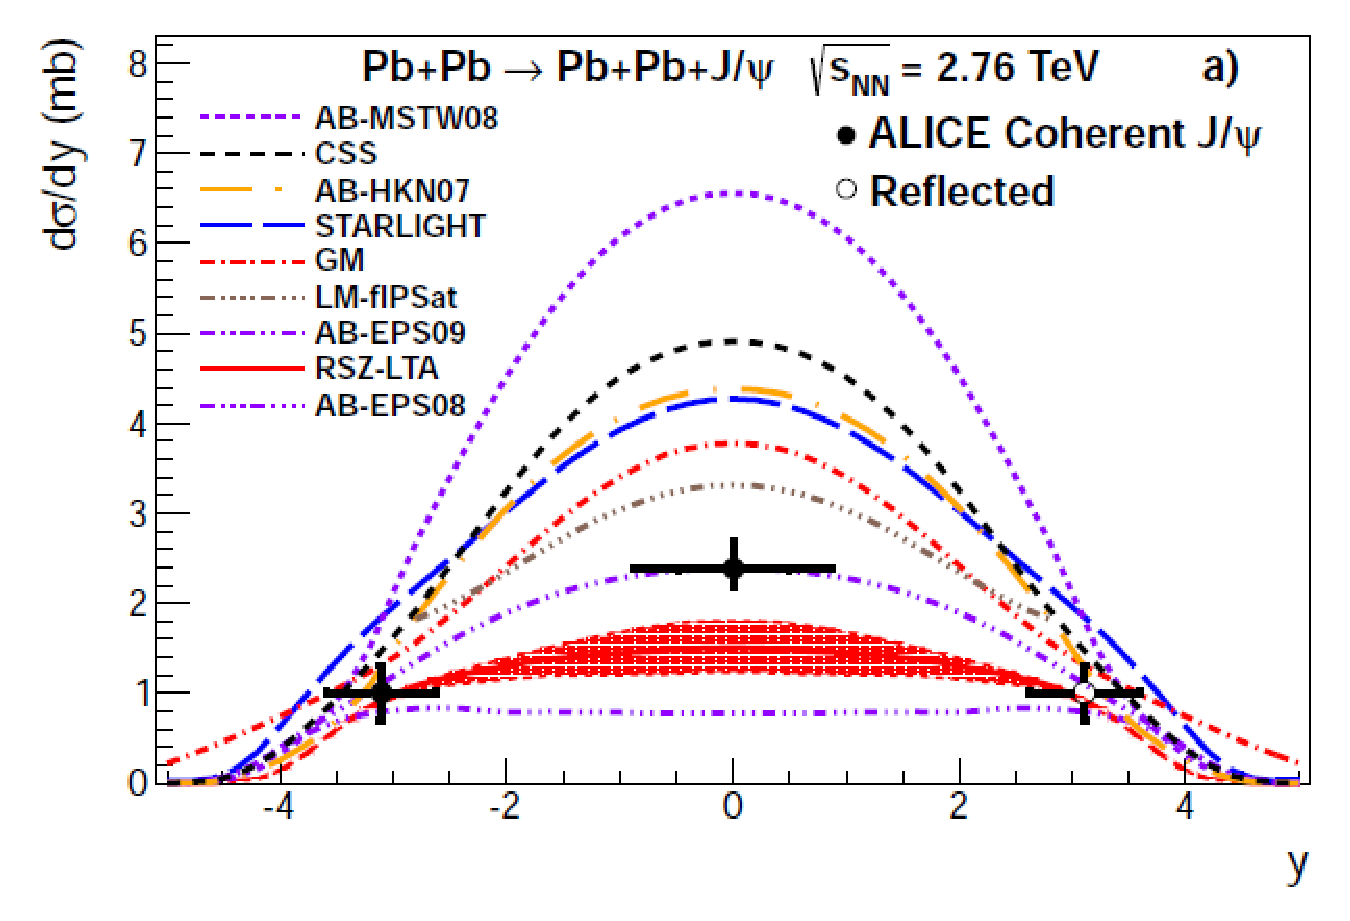
\includegraphics[width=.65\textwidth]{aliceJpsiCo}
      \caption{Coherent \JPsi{} photoproduction cross section in ultra-peripheral
        PbPb collisions at $\sqrt{s_{NN}}$ = 2.76 TeV, measured by the ALICE 
        experiment at forward and mid-rapidity~\cite{Abelev:2012ba,Abbas:2013oua}.}   
      \label{fig:aliceMoney}
    \end{figure}

    The ALICE data points have been compared to several theoretical models. 
  The UPC photoproduction cross section calculations depend significantly on 
    how the nucleus is represented in the calculation. 
  The results from the STARlight, LTA, and AB methods vary from a relatively 
    large cross section in the STARlight model, ranging through a variety of values
    in the AB method, to a relatively small cross section in the LTA method. 
  Each of these methods utilizes the same probe of the nucleus, the equivalent 
    photon flux that is calculated using the Weizs\"{a}cker-Williams approximation 
    (see Section~\ref{sec:wwAprox}). 
  The three methods deviate in how they calculate the forward photoproduction
    scattering cross section.
  The differences in the UPC photoproduction cross sections predicted by the 
    different models demonstrates the amount of experimental sensitivity there 
    is to distinguishing between the models. 
  The dependence of the cross section on rapidity is clearly visible.   

  The cross section value calculated by Eq.~\ref{eq:finalSTARlightResult} in the 
    STARlight, LTA, and the various gluon density models in AB method vary 
    significantly.
  Table~\ref{tab:allXsec} gives the predicted values for the three main methods
    taken from \cite{pQCD2013.02}, \cite{lta2011.09}, and \cite{vmd1999}.
  \begin{table} 
   \centering
   \begin{tabular}{|l|l|} 
     \hline
     Model & $\sigma_{AA\rightarrow AAJ/\psi} (mb)$ \\ \hline \hline
     STARlight/STARlight MC & 23 \\ \hline
     LTA & 9 \\ \hline
     AB-MSTW08 & 34 \\ \hline
     AB-EPS08 & 7  \\ \hline
     AB-EPS09 & 14 \\ \hline
     AB-HKN07 & 23 \\ \hline
     \hline
   \end{tabular}
   \caption{$\sigma_{AA\rightarrow AAJ/\psi} (mb)$
   obtained by the LTA, STARlight, AB methods for PbPb collisions at $\sqrt{s_{NN}}$ = 2.76 TeV. 
    Four different gluon density models~\cite{pQCD2011.08,pQCD2013.02,Pumplin:2002vw} are used 
    in the AB method. STARlight is a simulation software package that utilizes 
    the STARlight model.}
   \label{tab:allXsec}
  \end{table}
  The cross sections in Table~\ref{tab:allXsec} differ by a factor of 4 
    from the smallest to largest and create an experimental opportunity. 

  The nuclear suppression factor, S, demonstrates the difference between how 
    the models represent the nucleus. 
  $S$ is the ratio between the nuclear photoproduction cross section and the     
    free nucleon photoproduction cross section.
  It is a measure of how the nuclear gluon densities evolve in each of the 
    models. 
  Figure.~\ref{fig:ltaAndPqcdNucSub} from \cite{lta2013.05} shows the nuclear 
    suppression, which is equivalent to $R_g$ in Eq.~\ref{eq:ltaOptTheWNucMo}, 
    for the LTA and AB methods.
  \begin{figure}[h] 
    \begin{center}
      \includegraphics[width=0.5\textwidth,keepaspectratio]{ltaAndPqcdNucSub.png}
    \end{center}
    \caption{ \label{fig:ltaAndPqcdNucSub} Both panels show the nuclear 
      supression factor, $S$, obtain from the ALICE data points and calculations
      by the AB (top) and LTA (bottom) models~\cite{lta2013.05}. $S$ is denoted 
      as $R_{pb}$ in this figure.}
  \end{figure}
  \begin{figure}
    \begin{center}
      \includegraphics[width=0.5\textwidth,keepaspectratio]{ltaAndPqcdNucSubVMD.png}
    \end{center}
    \caption{ \label{fig:ltaAndPqcdNucSubSTARlight} Nuclear supression factor, $S$, in STARlight \DIFdelbeginFL \DIFdelFL{method}\DIFdelendFL \DIFaddbeginFL \DIFaddFL{model}\DIFaddendFL ~\cite{lta2013.05}.
      The y-axis is labeled $S$ because for the STARlight model $S$ is not 
      \DIFdelbeginFL \DIFdelFL{necessary }\DIFdelendFL \DIFaddbeginFL \DIFaddFL{necessarily }\DIFaddendFL equal to $R$.}
  \end{figure}
  Fig.~\ref{fig:ltaAndPqcdNucSubSTARlight} shows the nuclear suppression for the 
    STARlight method \cite{lta2013.05}. 
  \DIFaddbegin \DIFadd{$S$ is not directly related to the gluon density because the STARlight 
    uses a Glauber approach, which uses the $\gamma-p$ photoproduction 
    cross section rather than the nuclear gluon density directly.
  }\DIFaddend Fig.~\ref{fig:ltaAndPqcdNucSub} and Fig.~\ref{fig:ltaAndPqcdNucSubSTARlight} 
    show that as the momentum of the probing photon goes up, increasing 
    $W_{\gamma p}$, and momentum of the probed gluon goes down, decreasing $x$, 
    the nuclear gluon density decreases relative to the free nucleon. 
  The nuclear suppression factor, $S$, allows for the different models' 
    representations of the gluon content of the nucleus to be directly compared
    to each other and to data. 
  $S$ can be measured from data by assuming a Weizs\"{a}cker-Williams photon flux and 
    provides insight into nuclear gluon densities.

  In addition, ALICE reported the measurement of the incoherent \JPsi{} 
    photoproduction cross section at mid-rapidity~\cite{Abbas:2013oua}.
  This provided additional constraints to the models for gluon shadowing. 

  In Chapter~\ref{ch:analysis}, the coherent UPC \JPsi{} photoproduction 
    cross section using CMS is described.
  The measurement in this thesis adds to existing ALICE results, covering
    an intermediate range of $x$ values. 

  \include{diffDet}
  \include{diffZdc}
  \include{diffTrig}
  \chapter{Analysis}
  In the following chapter the various parts of the measurements done for this
    thesis are explained. 
  The following chapter contains seven sections explain each of these parts: 
    mc simulation, trigger development, data sets and event selection,
    break-up determination, signal extraction, efficiency determination,
    and systematic checks. 
  In Section~\ref{sec:mcSim} the simulations used to estimated the detectors 
    ability to measure UPC processes is discussed. 
  Section~\ref{sec:TrigDev} explains the considerations that went into the 
    triggers which were developed for the analyses discussed in this thesis.
  How the final events were selected and how triggers were used to separate the
    data in to data sets is detailed in Section~\ref{sec:DataSetEvSel}.
  Extraction of the number of events from each of the three physics processes 
    discussed in this thesis, coherent, incoherent, and photon-photon process
    from the final selected events is discussed is Section~\ref{sec:sigEx}.
  The estimates of the detectors efficiency for measuring UPC events is 
    explained in Section~\ref{sec:effDet}.
  Section~\ref{sec:sysCheck} lays out how the systematic uncertainties are 
    estimated.

  \section{\label{sec:mcSim} MC Simulation}
    Every physical measurement is the product of the underlying physics 
      convolved with the response of the detector used to do the measurement. 
    In order to understand the underlying physical process, the detector's 
      effect on the measurement must be understood and accounted for. 
    As instruments become more and more complicated, the interplay between all
      of the many parts of the detector makes an analytic approach to the 
      problem untenable.
    For this reason, the numerical technique of Monte Carlo (MC) simulation is
      the most useful approach.

    MC simulations use random number generation to solve the problem 
      numerically by brute force. 
    First, particles are generated according the theoretical distributions.
    These particles are then propagated through a simulation of the detector.
    As the particles pass through the detector, random numbers are again used
      to determine how these particles interact with the materials of the 
      detector based on the known properties of the material. 
    In this way, the theoretical distributions are merged with the complicated 
      response of the detector. 
    The collective combination of the many sub detectors responses with the 
      theoretical distributions emerges from the successive creation of random
      events.
    The result is the convolved response of the detector with the underlying 
      physical process that is to be studied. 

    In this thesis, two main classes of MC simulation samples were used. 
    The first class uses STARlight to generate events.
    This class of MC samples corresponds to the theoretical calculations 
      described in in Section~\ref{sec:vdmTheory}.
    There are three different physical process described.
    Coherent J/$\psi$ production, where the photon couples to the nucleus as
      a whole, incoherent J/$\psi$ production, where the photon couples to a
      nucleon within the nucleus, and photon-photon process, where the photons
      from the two nuclei interact with each other to produce a lepton pair 
      directly.
    All three STARlight sample produce a $\mu^{+}$ and $\mu^{-}$ in the final 
      state that interacts with the detector.
    The second class uses PYTHIA6 to decay \DIFdelbegin \DIFdel{$J/\psi$}\DIFdelend \DIFaddbegin \DIFadd{J/$\psi$}\DIFaddend s with a given
      input $p_{T}$ and rapidity distribution.
    Two samples of this class of particle gun data were produced each with 
      different $p_{T}$ distributions (See Fig.).

    The software chain used for producing the STARlight samples has five steps.
    Because STARlight is not integrated into the standard CMS software 
      framework (CMSSW), this chain was developed for the analysis described in this
      thesis.
    First, STARlight is run in the specified mode, and a single file is 
      created for each physics process, for this thesis, one file for the 
      coherent process, the incoherent process, and the photon-photon process
      for a total of three files.
    The output from the STARlight generator is in a format specific to 
      STARlight, therefore, the output from the original generation step is 
      then converted to the Les Houches (LHE) format. 
    In this conversion to LHE format, either the parent J/$\psi$ for the 
      J/$\psi$ production samples, or the initial photon-photon pair are added
      to the LHE output file.
    The standard STARlight output only includes the final state particles.
    Additionally, the initial output from STARlight is split into a collection 
      of smaller LHE files so that each of the smaller samples can be 
      processed in parallel.
    Each of the LHE files is used as input to CMSSW.
    The three remaining steps take place within the frame work. 
    First the generated particles are propagated through the GEANT4 detector 
      simulation.
    This accounts for all the interactions with the detector and produces as 
      output a format identical to the raw data that is recorded during data
      taking.
    The next two steps are identical to data taking.
    The reconstruction software used during data taking is run on the output 
      of the detector simulation, and last, the output of the reconstruction
      is reduced to the information that is needed for the final analysis.

    The particle gun samples were created entirely within CMSSW.
    An interface to PYTHIA6 is included within CMSSW, which takes J/$\psi$
      $p_{T}$ and rapidity distributions as input. 
    The J/$\psi$ are created according to the input distributions, and then uses
      PYTHIA6 to decay the J/$\psi$s to $\mu^{+}$ and $\mu^{-}$.
    As with the STARlight samples, these muons are propagated through the GEANT4
      simulation of the detector, and the raw data is produced.
    The remaining steps of running the reconstruction code and reducing the 
      data to the final data needed for the analysis are identical to the 
      STARlight production.

    The five MC samples, three STARlight samples, and two particle gun samples,
      differ primarily in the $p_{T}$ distribution of the J/$\psi$s produced
      and the polarization of the J/$\psi$s, which effects angle at which
      the muon daughters are emitted relative to the direction in which the
      J/$\psi$ is traveling. 
    In Fig.~\ref{fig:starlightRapPtDist} the $p_{T}$ of J/$\psi$s from the 
      coherent and photon-photon samples are peaked steeply a low $p_{T}$, and 
      neither sample extends much beyond 0.15 GeV in $p_{T}$.
    The incoherent sample is peaked near 0.5 GeV and extends beyond 1 GeV.
    The two particle gun samples resemble the incoherent and coherent samples.
    The first sample has a Gaussian $p_{T}$ distribution extending to 
      approximately 0.15 GeV, whereas the second is flat in $p_{T}$ up to
      2 GeV.
    The particle gun samples are unpolarized, whereas the STARlight samples 
      have transverse polarization. 
    Therefor, the particle gun samples there is no preferred direction for the 
      emission of the daughter muons.
    In the STARlight samples however the daughters tend to be emitted in line
      with the direction of the J/$\psi$'s momentum.
    This is particularly pronounced for the photon-photon process.

    \begin{figure}[!Hhbt]
      \centering
      $ \begin{array}{cc}
        \includegraphics[width=0.45\textwidth]{genRapDis} &
        \includegraphics[width=0.45\textwidth]{genPtDis}
      \end{array} $
      \caption{Generator level rapidity (left) and $p_{T}$ (right) 
          distributions for the coherent, \textcolor{red}{incoherent}, 
          and \textcolor{green}{photon-photon} process}
      \label{fig:starlightRapPtDist}
    \end{figure}

    \begin{figure}[!Hhbt]
      \centering
      \includegraphics[width=.6\textwidth]{polCosThetaHXGen}
      \caption{ The J/$\psi$ polarization of the \textcolor{red}{particle gun}
        , \textcolor{blue}{coherent}, and incoherent samples are plotted as the
        cosine of the helicity angle.} 
      \label{fig:genHXAngle}
    \end{figure}

    The momentum of the final state muons is the main drivers of whether the 
      candidate can be measured. 
    The polarization and the $p_{T}$ distribution of dimuons from the generator
      determine the momentum of the daughters. 
    The low $p_{T}$ of the J/$\psi$ restricts the momentum of the $\mu^{+}$ and
      $\mu^{-}$ daughters produced from the J/$\psi$ decay. 
    The polarization effects how the momentum is shared between the daughters.
    In the rest frame of the parent particle from which the daughters decay
      equal momentum is given to each daughter. 
    However in the lab frame of the detector, the muon daughters which are 
      emitted from transversely polarized J/$\psi$ will tend to be emitted in
      the direction of J/$\psi$ and will have unequal momentum in the lab 
      frame.
    The daughter traveling in the direction of the J/$\psi$ will have increased
      momentum, whereas the daughter traveling opposite to the J/$\psi$ 
      direction will have decreased momentum. 
    The combination of these two effects create a muon with very low momentum 
      compared to the typical momenta of muons measured by CMS. 
    The momentum of the lower momentum muon daughters is the main restriction
      on whether or not the J/$\psi$ can be measured. 

  \section{\label{sec:TrigDev} Trigger Development} 
    Prior to the 2011 LHC PbPb run, UPC events had not been directly studied in 
      PbPb collisions using CMS. 
    Design of the UPC triggers required studies of the 2010 data to estimate 
      rates and insure that the bandwidth used by these trigger would be
      sufficiently low. 
    All the different physics analyses must share the limited readout rate of 
      the detector.
    For this reason, conservation of bandwidth was a major design consideration.

    To estimate the 2011 rates prior to the run, the 2010 rates were used to 
      extrapolate to the interaction rate of the 2011 run. 
    The unique UPC triggers were estimated by combining existing triggers from
      the 2010 run. 
    By calculating the ratio between the UPC trigger rates and the minimum bias
      trigger rate, the UPC trigger rates were scaled up to the 2011 
      interaction rates using the 2010 data. 
    The extrapolated rates allowed for a package triggers to be created that 
      fit within the bandwidth requirement of CMS Heavy Ions group. 

    The trigger package for 2011 contained ZDC based efficiency monitoring 
      triggers, muon and electron based triggers for measuring \DIFdelbegin \DIFdel{$J/\psi$}\DIFdelend \DIFaddbegin \DIFadd{J/$\psi$}\DIFaddend , and 
      backup triggers in case there was a problem with the original muon and 
      electron triggers.
    In order to recorded the trigger efficiency monitoring data, the ZDC 
      triggers had to be prescaled to a lower rate. 
    The scaling down of the monitoring triggers were setup to insure overlap
      with the signal triggers.
    By balancing the competing objectives of rate reduction and increasing 
      the overlap between the monitoring and signal triggers, 
      the prescales for the trigger were as seen in Table .%~\ref{triggerTabel2011}.

    \subsection{\label{sec:l1Trigger} L1 Trigger}
      The goal of the L1 triggers was to record enough data to measure dimuons
        and dielectrons in UPC events.
      To achieve this, the loosest muon trigger and lowest threshold ECAL 
        triggers where paired with a trigger on energy in the ZDC and a veto on
	      energy in the BSC.
      Additional triggers which vetoed on energy in HF were commissioned in case
        radiation damaged to the BSCs.
      The L1 package that was constructed for the analysis of UPC \DIFdelbegin \DIFdel{$J/\psi$ 
        }\DIFdelend \DIFaddbegin \DIFadd{J/$\psi$ 
        }\DIFaddend is presented in Table~\ref{tab:l1Triggers2011}.

      \begin{table}[h]
        \centering
        \begin{tabular}{|l|l|}
          L1 Trigger Seed  & Type \\ \hline \hline
          L1\_MuOpen\_ZdcCalo\_NotBscMinBiasThresh2\_BptxAND & Physics \\  \hline
          L1\_EG2\_ZdcCalo\_NotBscMinBiasThresh2\_BptxAND & Physics \\  \hline
          L1\_EG5\_ZdcCalo\_NotBscMinBiasThresh2\_BptxAND & Physics \\ \hline
          L1\_ZdcCaloMinus\_BptxAND & Monitor \\  \hline
          L1\_ZdcCaloMinus\_BptxAND & Monitor \\  \hline
          L1\_MuOpen\_ZdcCalo\_NotHcalHfCoincidencePm\_BptxAND & Backup \\ \hline
          L1\_EG2\_ZdcCalo\_NotHcalHfCoincidencePm\_BptxAND & Backup \\ \hline
          L1\_EG5\_ZdcCalo\_NotHcalHfCoincidencePm\_BptxAND & Backup \\ \hline \hline
        \end{tabular}
        \caption{List of 2011 L1 seeds.}
        \label{tab:l1Triggers2011}
      \end{table}

      The cumulative L1 trigger rate for all the UPC L1 trigger seeds was
        required to be 200 Hz.
      This requirement stemmed from the need to keep the tracker read-out rate
        low. 
      The trackers baseline voltage can fluctuate due to the high tracker hit 
        multiplicities in PbPb collisions.
      In order to monitor the zero suppression of the tracker, the zero 
        suppression algorithm was executed using the HLT computing farm 
	      rather than the in the tracker firmware.
      The rate at which the tracker could be readout without zero suppression
        set the limit for the L1 bandwidth.


    \subsection{HLT Trigger}
      As opposed to the L1 trigger, which reads out the tracker, the HLT has 
        access to the tracker information. 
      Reconstruction of a track in the pixel detector is used by the UPC paths.
      The use of the pixel detector only, as opposed to using the whole tracker 
        including the silicon strip detector, allows for quick track 
        reconstruction saving computing cycles.
      The requirement of at least one reconstructed pixel track for the HLT 
        triggers was designed to reject backgrounds where no particles are 
        reconstructed by the tracker. 
  \begin{table}[h]
		\centering
		\begin{tabular}{|l|l|}
		  \hline HLT Trigger  \\ \hline \hline
		  HLT\_HIUPCNeuMuPixel\_SingleTrack & Physics   \\ \hline
		  HLT\_HIUPCNeuEG2Pixel\_SingleTrack & Physics   \\ \hline
		  HLT\_HIUPCNeuEG5Pixel\_SingleTrack & Physics   \\ \hline
		  HLT\_HIMinBiasZDC\_Calo\_PlusOrMinus\_v1  & Monitor  \\ \hline
		  HLT\_HIMinBiasZDC\_PlusOrMinusPixel\_SingleTrack\_v1   & Monitor \\ \hline
		  HLT\_HIUPCNeuHcalHfMuPixel\_SingleTrack & Backup   \\ \hline
		  HLT\_HIUPCNeuHcalHfEG2Pixel\_SingleTrack & Backup   \\ \hline
		  HLT\_HIUPCNeuHcalHfEG5Pixel\_SingleTrack & Backup   \\ \hline \hline
		\end{tabular}
		\caption{List of 2011 HLT trigger.}
		\label{tab:hltTriggers2011}
	\end{table}

      The total HLT output for the UPC trigger package was 20 Hz. 
      The limiting factor for the HLT rate was the amount of disk space 
        available to store the data. 
      To meet the bandwidth the requirements and collected a significant sample
        of data for estimating efficiencies, the prescales for the triggers 
        were set. 
      The ZDC trigger that was passed through from the L1 was given a larger 
        prescale to account for the higher rate relative to the more selective 
        ZDC path, which also required a pixel track on the HLT.

  \section{\label{sec:DataSetEvSel} Data Sets and Event Selection}
    In order to investigate novel physics processes like UPC \DIFdelbegin \DIFdel{$J/\psi$ 
     }\DIFdelend \DIFaddbegin \DIFadd{J/$\psi$ 
     }\DIFaddend production, the LHC has delivered unprecedented amounts of data.
    The data for this analysis was recorded during the 2011 LHC PbPb run. 
    During this period, 150 $\mu$$b^{-1}$ where recorded by the CMS detector,
      corresponding to over a billion PbPb collisions. 
    Of this, 143 $\mu$$b^{-1}$ are used in this analysis.

    \subsection{Data Set}
      Three specially selected samples were used for the present analysis 
        (see Table~\ref{tab:sampleLumiNevt}).
      These samples were recorded using subsets of the triggers found in 
        Section~\ref{sec:TrigDev}.
      The \DIFdelbegin \DIFdel{$J/\psi$ }\DIFdelend \DIFaddbegin \DIFadd{J/$\psi$ }\DIFaddend events discussed in this thesis were obtained analyzing the 
        sample labeled in Table~\ref{tab:sampleLumiNevt} as physics.
      A ZDC triggered sample was recorded for the sake of estimating 
        efficiencies.
      Last, a zero bias sample was recored for investigating the ZDC and the 
        noise distributions of HF.
      By recording this hierarchy of samples, interesting events are selected 
        with a much higher purity in the physics sample, while the zero bias and 
      ZDC triggered samples allow for the investigation of the selection 
        criteria. 

      To record the physics sample containing the \DIFdelbegin \DIFdel{$J/\psi$ }\DIFdelend \DIFaddbegin \DIFadd{J/$\psi$ }\DIFaddend signal, a muon trigger
        was paired with a veto on energy in the BSC and a requirement that there 
        be energy in at least one of two sides of the ZDC. 
      This trigger utilizes the unlikely chance of having overlapping noise in
        in the ZDC and muon detector.
      Because of the characteristically low momentum of UPC \DIFdelbegin \DIFdel{$J/\psi$ }\DIFdelend \DIFaddbegin \DIFadd{J/$\psi$ }\DIFaddend as compared
        to \DIFdelbegin \DIFdel{$J/\psi$ }\DIFdelend \DIFaddbegin \DIFadd{J/$\psi$ }\DIFaddend created by other physics process, the loosest muon 
        trigger was used.
      By pairing the muon trigger with the ZDC on the L1, the noise contribution
        was reduced from the noise contribution from either of the two 
        sub-detectors to the noise coincidence between the two sub-detectors. 
      Contributions from hadronic interactions are reduced by the veto on the 
        BSC.
      In this way the balance between reducing the rate and maximizing the 
        efficiency was struck, allowing for the data to be recorded without 
        producing high rates resulting in dead time for the detector.  

      In order to investigate the muon trigger and the other parts of the event 
        selection, a minimum bias sample was recorded using the ZDC. 
      For ZDC triggered sample, any event which had energy consistent with at 
        least one neutron in either of the two sides of the ZDC was recorded.
      This process is much more common than the UPC \DIFdelbegin \DIFdel{$J/\psi$ }\DIFdelend \DIFaddbegin \DIFadd{J/$\psi$ }\DIFaddend production.
      For this reason, the rates of this trigger are much higher than the physics
        trigger, and only a small sub set of these events are recorded.
      From this trigger the pixel track portion of the HLT trigger efficiency 
        was estimated. 

      In addition to the minimum bias and physics sample, a zero bias sample was 
        recorded to examine the ZDC trigger and the HF noise distributions. 
      The zero bias trigger fired every time both beams passed through CMS. 
      Only 4 events out of every million triggered were recorded for this sample. 
      This sample allowed for an unbiased measurement of the ZDC trigger 
      efficiency as discussed in Section~\ref{sec:effDet}. 
      Because the zero bias trigger does not require any activity in any of the
        CMS sub detectors, the sample contains very few hadronic collisions. 
      This allowed for a measurement of the electronic noise distributions in
        the HF, which will be discussed in the next section.

      The integrated luminosity for each of the three samples is calculated
      by recording activity in HF \DIFaddbegin \DIFadd{\mbox{%DIFAUXCMD
\cite{cmsLumi}
}%DIFAUXCMD
}\DIFaddend . 
      The cross section for HF activity is measured from a van der Meer scan, 
        and the cross section was found to be \textcolor{red}{X}.
      In this way the amount of integrated luminosity for any running period is
        related to the activity in HF. 
      \begin{table}
  	    \centering
  	    \begin{tabular}{|l|l|l|}
  	      \hline Sample & Events & $L_{int}$ \\ \hline \hline
  	      Physics & \textcolor{red}{300K} & \textcolor{red}{143.3 
  	        $\mu$$b$} \\ \hline
  	      Minimum Bias & \textcolor{red}{100K} & \textcolor{red}{X} \\ \hline
  	      Zero Bias & \textcolor{red}{5M} & \textcolor{red}{580 b} \\ \hline \hline
  	    \end{tabular}
  	    \caption{Integrated luminosities and number of events for the three
  	      samples used in this analysis.}
  	    \label{tab:sampleLumiNevt}
      \end{table}
      An additional method was used to cross check the integrated luminosity 
        obtained by the van der Meer scan technique.
      The integrated luminosity can also be measured by counting the events that
        fire the L1 minimum bias trigger together with the inelastic PbPb cross 
        section. 

    \subsection{Event selection}
      The analysis described in this thesis focuses on UPC \DIFdelbegin \DIFdel{$J/\psi$}\DIFdelend \DIFaddbegin \DIFadd{J/$\psi$}\DIFaddend s decaying to 
        muons. 
      The trigger used for this analysis recored 346841 events.
      A set of off-line cuts were applied to increase the relative contribution 
        of UPC events to background processes. 
      The following cuts were applied. 

      \begin{table}
        \centering
        \begin{tabular}{|c|c|c|} \hline 
          cut & cut type & events \\ \hline
          all triggered & -- & 346841 \\ \hline
          good vertex requirement & beam background rejection & 340997 \\ \hline
          beam halo muon rejection & beam background rejection & 302777 \\ \hline
          cluster shape compatibility requirement & beam background rejection & 233590 \\ \hline
          single-sided neutron requirement & hadronic interaction rejection & 149992 \\ \hline
          two track requirement & hadronic interaction rejection & 32732 \\ \hline
          HF signal rejection & hadronic interaction rejection & 5392 \\ \hline
          muon quality requirement & fake muon rejection & 1956\\ \hline
          J/$\psi$ mass requirement & kinematic cut & 662 \\ \hline
          muon detectability cuts & kinematic cut & 541 \\ \hline
        \end{tabular}
        \caption{Effects of event selection cuts.}
        \label{tab:evSelCutNumbers}
      \end{table}

      Two sets of event selection cuts were applied to reject background events. 
      The first set rejects background from the beam.
      The second rejects events where hadronic collisions have occurred.

      To reject beam induced background the following cuts were applied:
      \begin{itemize}
        \item The reconstructed vertex must be within \textcolor{red}{X} cm in 
          the transverse direction and \textcolor{red}{X} cm in the 
          longitudinal direction. This cut insures that reconstructed particles 
          come from interactions between the two beams rather than event where 
          one of the two beams interact with gas particles near the interaction 
          point. 
  	    \item Beam halo muons were rejected using the timing of the muon hits.
              The beam halo cut rejects events where muons surrounding the beam 
              stream through the detector. 
  	    \item Pixel cluster shape should be compatible with the vertex. 
          This cut requires that energy deposits in the silicon tracker point 
            back to the reconstructed  primary vertex. 
      \end{itemize}
      These beam background cuts do not reject any UPC J/$\psi$ candidates. 

      The second set of background rejection cuts were designed to 
        reduce contamination from hadronic interactions. 
      \begin{itemize}
  	    \item No more than 2 reconstructed tracks in the event.
          The track requirement rejects events that produce many charged 
          particles.
  	    \item Maximum reconstructed hit energy in HF was required to be below 
            the threshold for electronic noise. 
          Nearly all hadronic interactions ($\sim$ 98\%) produce particles in 
            the range $3<|\eta|<5$ covered by the HF detector.
          By requiring that the energy deposits in HF resemble noise, nearly all
            elastic hadronic collisions are expected to be rejected.
  	    \item Energy in the ZDCs consistent with neutrons on only one side 
            of the interaction point.
          In hadronic interactions both nuclei break-up. 
          By requiring that ZDC only reconstruct neutrons on one side of the 
            interaction point, hadronic interactions that produce neutrons on 
            both sides were rejected.
      \end{itemize}
      Each of these cuts are designed to reject topologies produced by hadronic
        interactions.
      The effect of these cuts can be seen in Table\textcolor{red}{X}.

      To establish the HF noise thresholds, the noise distributions were 
        measured in zero bias events. 
      Only presences of both beams was required for these events to be recorded. 
      An Off-line selection of events with no reconstructed tracks was used
        to insure that no collision had taken place. 
      The HF noise threshold was defined as the cut that keeps \%99 of the 
        zero bias events.
      The noise distribution from this zero bias sample is compared to the 
        physics sample and MC in Fig.~\ref{fig:hfNoiseDist}.

      \begin{figure}[!Hhbt]
        \centering
        \includegraphics[width=.6\textwidth]{hfNoiseComp}
        \caption{Comparison of HF noise distributions in zero bias data, 
          physics triggered data, and MC.}
        \label{fig:hfNoiseDist}
      \end{figure}

      The following standard muon quality cuts are applied:
      \begin{itemize}
        \item Tracker track matched with at least one muon segment 
          (in any station) in both X and Y coordinates (< 3 $\sigma$).
        \item Cut on number of tracker layers with hits $>$ 5.
        \item Number of pixel layers $>$ 0.
        \item The $\chi^{2}$ per degrees of freedom of the track fit $<$ 3. 
        \item Loose transverse and longitudinal impact parameter cuts, with in 3 
          cm in the transverse direction and withing 30 cm in the longitudinal 
          direction with respect to the primary vertex.
      \end{itemize}
      These cuts are applied to reduce the number of fake muons.

  \section{\label{sec:breakUpDet} Break up determination}
    As described in Section\DIFdelbegin \DIFdel{.}\DIFdelend ~\ref{sec:ltaTheory}, UPC J/$\psi$ photoproduction 
      can be accompanied by the emission of neutrons from either of the two 
      colliding nuclei.
    The various neutron emission scenarios, or break-up \DIFdelbegin \DIFdel{break up }\DIFdelend modes, can 
      be distinguished by the ZDC.
    By separating events where the ZDC signal is consistent with 1 neutron 
      versus several neutrons, the different break-up modes can be separated
      and compared to theory. 
    For this reason, reconstruction of the ZDC signal plays an important role 
      in this thesis. 
    In order to maximize the ability to explore the one neutron peak, which 
      sits at the bottom of the ZDCs dynamic range, a new ZDC reconstruction 
      method was devised. 
    This new reconstruction method was \DIFdelbegin \DIFdel{than }\DIFdelend \DIFaddbegin \DIFadd{then }\DIFaddend used to establish a one neutron and
      many neutron threshold.
    In this section the ZDC signal reconstruction is described and how the 
      neutron thresholds on this signal were set.

    \subsection{ZDC \DIFdelbegin \DIFdel{Signal Reconstruction}\DIFdelend \DIFaddbegin \DIFadd{signal reconstruction}\DIFaddend }
      The ZDC signal is built up from the pulse shapes for each of the 
        18 individual ZDC channels. 
      The pulse shape is recorded in 250 ns second chunks and is divided into
        10 time slices of 25 ns (See Fig~\ref{fig:zdcPulseShape}).
      Counting from 0, the 4th time slice is synced with the timing of the rest
        of the detector and corresponds to when the products of the recorded 
        collision reached the ZDC.
      For this reason the channel signal is taken from the 4th time slice.
      \begin{figure}[h]
        \centering
        \includegraphics[width=\textwidth]{zdcPulseShape}
        \caption{\DIFaddbeginFL \DIFaddFL{Average }\DIFaddendFL ZDC pluse shape \DIFaddbeginFL \DIFaddFL{is plotted as the charge as a function
          of time slice for the first hadronic from ZDC$^{-}$ (left) and 
          ZDC$^{+}$ (right)}\DIFaddendFL .}
        \label{fig:zdcPulseShape}
      \end{figure}

      The ZDC signal sits on top of a low frequency noise pedestal. 
      Over the time scale of 250 ns, this low frequency noise signal appears
        as a constant that shifts randomly from event to event.
      The contribution from this noise is therefore measured event by event
        in order to subtract it.
      Time slice 5 is used for this purpose.

      Time slices 1 and 2 could also be used to estimate the low frequency 
        noise.
      However because the noise fluctuates to negative values of charge that 
        \DIFdelbegin \DIFdel{can't be measuredby the QIE}\DIFdelend \DIFaddbegin \DIFadd{cannot be measured}\DIFaddend , these time \DIFdelbegin \DIFdel{slice }\DIFdelend \DIFaddbegin \DIFadd{slices }\DIFaddend can only provide a 
        measurement \DIFaddbegin \DIFadd{of the noise }\DIFaddend half the time. 
      By using time slice 5 which contains the falling tail of the signal, 
        the noise can be measured any time the signal raises significantly 
        above the noise.
      If the fraction of signal in time slice 4 and 5 are constant and
        the noise contributes the same value to both time slices, the 
        following formula is applicable:
      \begin{equation}
        Ts4 \propto (Ts4 + C) - ( Ts5 + C ) = Ts4 - R_{Ts5/Ts4}\DIFdelbegin \DIFdel{*Ts4 
        }\DIFdelend \DIFaddbegin \DIFadd{Ts4 
        }\DIFaddend = Ts4(1-R_{Ts5/Ts4}),
        \label{eq:ts4ish}
      \end{equation}
      where $Ts4$ is the signal contribution in time slice 4, $Ts5$ is the 
        signal contribution to time slice 5, $C$ is a random noise constant
        from the low frequency noise, and $R_{Ts5/Ts4}$ is the ratio between
        the signal contribution from time slice 5 over time slice 4.
      Fig.~\ref{fig:zdcTs4OvTs5VTs5} demonstrates the consistence of the 
        fraction and validates the unconventional method of using the falling 
        tail of the signal to estimate the low frequency noise. 
      By using time slice 5\DIFdelbegin \DIFdel{the chances }\DIFdelend \DIFaddbegin \DIFadd{, the chances of }\DIFaddend measuring the noise are maximized\DIFdelbegin \DIFdel{allowing for the possiblity to sperate the }\DIFdelend \DIFaddbegin \DIFadd{. 
      Separating the }\DIFaddend signal from the noise \DIFdelbegin \DIFdel{and
        measure }\DIFdelend \DIFaddbegin \DIFadd{is especially important because
        }\DIFaddend the ZDC signal \DIFdelbegin \DIFdel{near }\DIFdelend \DIFaddbegin \DIFadd{for the one neutron peak sits near the }\DIFaddend noise at the 
        bottom of the ZDC dynamic range.
      \begin{figure}[!Hhbt]
        \centering
        $ \begin{array}{cc}
          \includegraphics[width=.4\textwidth]{negTs5overTs4vts5} &
          \includegraphics[width=.4\textwidth]{posTs5overTs4vts5}
        \end{array} $  
        \caption{ The fraction of signal in time slice 5 over time slice 4 
          as a function of the signal in time slice 5 in ZDC$^{-}$ (left) and 
          ZDC$^{+}$ (right).}
        \label{fig:zdcTs4OvTs5VTs5}
      \end{figure}

      To measure one signal value for ZDC$^{+}$ and one for ZDC$^{-}$, the 
        signals from each of the channels are combined.
      Channels from the EM section and HD section are combined first. 
      Only channels with signal above zero in time slice 5 and time slice 
        4 are included. 
      The EM section of the calorimeter is more densely packed with optical 
        fibers and therefore has a higher gain relative to the HAD section. 
      To account for this, the combination of EM channels is weighted with
        a factor of 0.1 to match the HAD channel gains.
      The value for each side of the ZDC's signal is given by the sum of the 
        HAD channel combination and weighted EM channel combination.
      It is this signal, one for ZDC$^{+}$ and one for ZDC$^{-}$, 
        which is plotted \DIFaddbegin \DIFadd{in Fig.~\ref{fig:zdcM2Fit} }\DIFaddend to measure the neutron 
        thresholds.

    \subsection{Determination of the one neutron thresholds}
      The ZDC thresholds used to establish the various break-up modes were 
        measured from zero bias data.
      By using this dataset, the \DIFaddbegin \DIFadd{neutron }\DIFaddend spectrum does not contain a trigger 
        bias. 
      \DIFdelbegin \DIFdel{The trigger requirement for the zero bias events is }\DIFdelend \DIFaddbegin \DIFadd{Zero bias trigger required }\DIFaddend that both beams were present in CMS.
      This does\DIFdelbegin \DIFdel{however }\DIFdelend \DIFaddbegin \DIFadd{, however, }\DIFaddend include a significant electronic noise contribution due
        to events where no neutrons are emitted in the direction of the ZDC.

      To determine the thresholds for one and multiple neutrons, the ZDC$^{+}$ 
        and ZDC$^{-}$ spectra \DIFdelbegin \DIFdel{are }\DIFdelend \DIFaddbegin \DIFadd{were }\DIFaddend fit.
      Four Gaussian functions were combined to fit the spectra. 
      The electronic noise was fit to a Gaussian \DIFdelbegin \DIFdel{about }\DIFdelend \DIFaddbegin \DIFadd{around }\DIFaddend zero.
      The one, two, and three neutron peaks are fit to Gaussians that are 
        successively broader.
      The mean of each peak was initially set to multiples of the mean of the 
        one neutron peak. 
      \begin{figure}[!Hh]
        \centering
        $ 
          \begin{array}{cc}
            \includegraphics[width=0.45\textwidth]{zdcFit45Neg} &
            \includegraphics[width=0.45\textwidth]{zdcFit45Pos}
          \end{array} 
        $
        \caption{Fit to the signal spectra for ZDC$^{-}$ (left) and ZDC$^{+}$ 
          (right)}
        \label{fig:zdcM2Fit}
      \end{figure}
      The threshold for a neutron in the ZDC was taken from the fits in 
        Fig.~\ref{fig:zdcM2Fit}.
      Any signal greater 2$\sigma$ below the mean of the one neutron peak was 
        considered signal.
      Any signal greater than 2$\sigma$ above was considered multiple 
        neutrons.
      In this way the single neutron break up modes could be separated from the
        multiple neutron modes.

      Several of the break-up mode calculations that have been done involve
        single sided configurations where neutrons are present on one side
        of the interaction point and not the other.
      To identify signal consistent with noise, noise distributions for the 
        combined EM sections and the combined HAD sections were measured.
      The beams are only made to collide every 200 ns. 
      In Fig.~\ref{fig:zdcPulseShape} higher than average signal can be seen
        in the 0th time slice, which precedes the main signal time slice 
        time slice 4 by 200 ns. 
      This is due to events where activity was present in the ZDC for 
        two consecutive collisions.
      Time slices 1 and 2, however, occurred between collisions.
      These time slices were used to estimate the noise spectrum.
      \begin{figure}[!Hhbt]
        \centering
        $ \begin{array}{cc}
          \includegraphics[width=.45\textwidth]{zdcNegEMNoiseFromZBNoCor} & 
          \includegraphics[width=.45\textwidth]{zdcPosEMNoiseFromZBNoCor} \\
          \includegraphics[width=.45\textwidth]{zdcNegHDNoiseFromZB} &
          \includegraphics[width=.45\textwidth]{zdcPosHDNoiseFromZB}
        \end{array} $
        \caption{ZDC noise spectra from ZDC$^{-}$ EM section (upper left), 
          ZDC$^{+}$ EM section (upper right), ZDC$^{-}$ HAD section (lower left), 
          and ZDC$^{+}$ HAD section (lower right).}
        \label{fig:zdcNoiseSpectra}
      \end{figure}

      Fig~\ref{fig:zdcNoiseSpectra} shows the noise spectrum for each of the 
        EM and HAD sections for the two sides of the ZDC. 
      As with the signal measurements, the low frequency noise pedestal is 
        subtracted event by event by subtracting time slice 2 from time slice
        one before the channel signals are combined for each section.
      A side is considered consistent with noise if both HAD section and EM 
        section signal measurements from the signal method involving time slice
        4 and time slice 5 are lower than 2 sigma below the mean in 
        Fig.~\ref{fig:zdcNoiseSpectra}.
      With the single \DIFdelbegin \DIFdel{nuetron}\DIFdelend \DIFaddbegin \DIFadd{neutron}\DIFaddend , multi-neutron, and noise thresholds established,
        the contributions to the various break-up modes were estimated and 
        compared to theory. 


  \section{\label{sec:sigEx} Signal extraction}
    After all event selection cuts, the coherent J/$\psi$, incoherent J/$\psi$,
      and photon-photon process all contribute to the remaining events.
    Each process must be separated from the final mix.
    To achieve this, the invariant mass and $p_{T}$ distributions are used 
      to distinguish between the three processes. 
    The photon-photon process is extended in invariant mass whereas the 
      J/$\psi$ is peak strongly near 3.1 GeV.
    In $p_{T}$ the photon-photon and coherent process have similar 
      distributions, both peaked shapely below 0.1 GeV, whereas the incoherent 
      process is more broadly distributed across an interval extending to 
      nearly 1 GeV.
    The mass distribution was \DIFdelbegin \DIFdel{fitted }\DIFdelend \DIFaddbegin \DIFadd{fit }\DIFaddend to separate the photon-photon process from
      the J/$\psi$ process.
    The $p_{T}$ distribution was used to separate the incoherent process from 
      the photon-photon process, and the coherent process. 
    In this way, a separate yield was extracted for all three processes. 

    The invariant mass distribution for opposite sign dimuons is shown in 
      Fig.~\ref{fig:massFit}. 
    A J/$\psi$ signal is clearly visible together with tails at higher and
      \DIFdelbegin \DIFdel{in
      }\DIFdelend lower mass due to the photon-photon process.
    A fit to the invariant mass distribution was done using a Gaussian
      to account for the J/$\psi$ signal and a first order polynomial function 
      for the photon-photon process.
    The extracted number of J/$\psi$ candidates from this fit includes all 
      J/$\psi$s in the mass window that passed the analysis cuts, i.e. both
      coherent and incoherent process contribute to yield from the mass
      fit.
    The $p_{T}$ distribution is needed to separate the two different 
      contributions to the J/$\psi$ peak. 

    \begin{figure}[!Hhtb]
      \centering
      \includegraphics[width=.6\textwidth]{massFitSimple}
      \caption{Mass fit to J/$\psi$ using Gaussian for the 
        signal and a first order polynomial for the photon-photon continuum}
      \label{fig:massFit}
    \end{figure}

    The same candidates from Fig.~\ref{fig:massFit} \DIFdelbegin \DIFdel{are }\DIFdelend \DIFaddbegin \DIFadd{were }\DIFaddend plotted as a function
      of $p_{T}$ in Fig.~\ref{fig:ptTemps}.
    The clear overlap of the coherent and photon-photon process, and the 
      clear separation of these two lower $p_{T}$ processes from the incoherent
      process \DIFdelbegin \DIFdel{are }\DIFdelend \DIFaddbegin \DIFadd{is }\DIFaddend apparent.
    The shape of the $p_{T}$ distribution for the coherent, incoherent, and 
      photon-photon process are taken from the final output of MC after
      applying all analysis cuts. 
    To obtain the yields for each of the three process, the $p_{T}$ 
      distribution was fit to the three templates.
    In Fig.\ref{fig:ptTemps}, the yield parameters that were fit were left
      unconstrained for all three process.

    \begin{figure}[!Hhbt]
      \centering
      \includegraphics[width=.6\textwidth]{ptOnly}
      \caption{ Fit to MC $p_{T}$ templates. }
      \label{fig:ptTemps}
    \end{figure}

    The shape of the photon-photon \DIFdelbegin \DIFdel{process }\DIFdelend and coherent J/$\psi$ \DIFaddbegin \DIFadd{process }\DIFaddend are very 
      similar in $p_{T}$.
    Accordingly, the contribution from the photon-photon process and the 
      coherent process are difficult to separate from the $p_{T}$ distribution.
    The confidence contours in Fig.~\ref{fig:ptOnlyCor} from the template fit
      in Fig.~\ref{fig:ptTemps} demonstrate the strong anti-correlation 
      between the coherent yield parameter, $nCo$, and the yield parameter 
      for the photon-photon process, $nGamma$.
    Because of the anti-correlation, the statistical uncertainty on $nCo$ and 
      $nGamma$ from the fit are larger than $\sqrt{nCo}$ and $\sqrt{nGamma}$
      expected from Poisson statistics. 
    The information from the invariant mass and $p_{T}$ distributions \DIFdelbegin \DIFdel{was 
      }\DIFdelend \DIFaddbegin \DIFadd{were
      }\DIFaddend combined to break this correlation. 
    Through this combination, the contribution to the final yield from 
      the three process was measured.

    \begin{figure}[!Hhbt]
      \centering
      \includegraphics[width=.6\textwidth]{nCoNGammaCorPtOnly}
      \caption{68\%, 95\%, and 99\% confidence contours from the $p_{T}$ 
        template fit. }
      \label{fig:ptOnlyCor}
    \end{figure}

    To utilize the mass fits ability to distinguish the photon-photon process 
      from the coherent and incoherent process all while utilizing the $p_{T}$
      fits ability to separate the coherent and photon-photon processes from 
      the incoherent, a simultaneous fit to the mass spectrum and $p_{T}$ 
      spectrum was preformed.
    Fig.~\ref{fig:simFitMassPtGauss} shows the result of the simultaneous fit.
    The simultaneous fit forces the parameter $nGamma$ to both describe the 
      photon-photon continuum present in the side bands of the J/$\psi$ mass 
      peak as well the photon-photon contribution to the low-$p_{T}$ part of 
      the $p_{T}$ spectrum.
    In addition, the J/$\psi$ yield from the mass fit is forced to equal the
      contribution from \DIFdelbegin \DIFdel{from }\DIFdelend the incoherent and coherent process in the 
      fit to the $p_{T}$ distribution. 
    In this way, the correlation between the yield parameters was broken, and 
      the contribution from the three process \DIFdelbegin \DIFdel{are left }\DIFdelend \DIFaddbegin \DIFadd{were made }\DIFaddend independent of each 
      other.

    \begin{figure}[!Hhbt]
      \centering
      \includegraphics[width=0.9\textwidth]{ptMassSimGaussLine}
      \caption{Simultaneous fit to the mass and $p_{T}$ spectra.}
      \label{fig:simFitMassPtGauss}
    \end{figure}

    \DIFdelbegin \DIFdel{By simultaneously fitting both the mass and $p_{T}$ spectra, the yields
      from the coherent, incoherent, and photon-photon process were separated 
      from each other in total yield of final candidates.
    }\DIFdelend The ambiguity between the coherent and incoherent processes in the mass fit
      \DIFaddbegin \DIFadd{and }\DIFaddend the ambiguity between the coherent and the photon-photon process was 
      over come \DIFdelbegin \DIFdel{by combining the two fits}\DIFdelend \DIFaddbegin \DIFadd{through used of the simultaneous fit}\DIFaddend .
    Fig.~\ref{fig:simGaussCor} shows the confidence contours for \DIFdelbegin \DIFdel{nCo and 
      nGamma
      }\DIFdelend \DIFaddbegin \DIFadd{$nCo$ and 
      $nGamma$ }\DIFaddend from the simultaneous fit in Fig.~\ref{fig:simFitMassPtGauss}.  
    The slope of the confidence contours in Fig.~\ref{fig:simGaussCor} 
      is noticeably closer to 0 than the apparent negative slope in 
      Fig.~\ref{fig:ptOnlyCor}.
    The contours for the simultaneous fit are also reduced compared to 
      Fig.~\ref{fig:ptOnlyCor} with widths in $nCo$ and $nGamma$ similar to 
      those expected from Poison statistics. 
    From the simultaneous fit, reasonable statistical errors were obtained 
      along with the yields for the three processes. 

    \begin{figure}[!Hhbt]
      \centering
      \includegraphics[width=0.6\textwidth]{nCoNGammaCorPtMass}
      \caption{68\%, 95\%, and 99\% confidence contours from the 
        simultaneous fit. }
      \label{fig:simGaussCor}
    \end{figure}

  \section{\label{sec:effDet} Efficiency determination}
    \subsection{Muon \DIFdelbegin \DIFdel{Efficiencies}\DIFdelend \DIFaddbegin \DIFadd{efficiencies}\DIFaddend }
      The muon efficiencies are measured from MC and data.
      The MC based measurement accounts for the detector acceptance and the 
        efficiency of the muon quality discussed in 
        Section~\ref{sec:DataSetEvSel}.
      The trigger efficiencies were measured in data using the tag and probe 
      method \DIFaddbegin \DIFadd{\mbox{%DIFAUXCMD
\cite{cmsTnP}
}%DIFAUXCMD
}\DIFaddend , which is discussed below. 

       CMS has a limited acceptance for \DIFdelbegin \DIFdel{$J/\psi$}\DIFdelend \DIFaddbegin \DIFadd{J/$\psi$}\DIFaddend s, particularly in the case of 
        \DIFdelbegin \DIFdel{$J/\psi$}\DIFdelend \DIFaddbegin \DIFadd{J/$\psi$}\DIFaddend s with low momentum like those produced in UPC events. 
      To measure the acceptance of CMS for \DIFdelbegin \DIFdel{$J/\psi$}\DIFdelend \DIFaddbegin \DIFadd{J/$\psi$}\DIFaddend s, reconstructed dimuon 
        candidates were considered detectable if both reconstructed daughters 
        fell into a detectability region.
      This region was defined using the coherent J/$\psi$ events obtained from 
        STARlight.
      The efficiency for reconstructing single muons $\varepsilon^{\mu}_{reco}$ 
        is defined by $\varepsilon^{\mu}_{reco} = \frac{N^{\mu}_{reco}}{N^{\mu}_{gen}}$, 
        where $N^{\mu}_{reco}$ is the number reconstructed muons \DIFdelbegin \DIFdel{after 
        after }\DIFdelend \DIFaddbegin \DIFadd{obtained 
        after }\DIFaddend the full CMS detector simulation and that \DIFdelbegin \DIFdel{pass }\DIFdelend \DIFaddbegin \DIFadd{passed }\DIFaddend the standard
        muon quality cuts, and $N^{\mu}_{gen}$ is the number of generated 
        muons from STARlight.
      \DIFdelbegin %DIFDELCMD < \begin{figure*}[!Hhtb]
%DIFDELCMD <         %%%
\DIFdelend \DIFaddbegin \begin{figure}[!Hhtb]
        \DIFaddendFL \centering
          %DIF <           $ \begin{array}{cc}
          \includegraphics[width=.6\textwidth]{mcEffMaps/accMuJpCo} 
        %DIF < &
    %DIF <       \includegraphics[width=.45\textwidth]{mcEffMaps/accMuJpInCo} \\
    %DIF <       \includegraphics[width=.45\textwidth]{mcEffMaps/accMuGamma} &
    %DIF <       \includegraphics[width=.45\textwidth]{mcEffMaps/accMuGun}
%DIF <          \end{array} $
        \caption{ Muon daughter detectability from coherent J/$\psi$\DIFdelbeginFL \DIFdelFL{, 
          incoherent J/$\psi$, photon-photon, and J/$\psi$ gun samples.}\DIFdelendFL }
        \label{fig:muonDaughterDet}
      \DIFdelbeginFL %DIFDELCMD < \end{figure*}
%DIFDELCMD <       %%%
\DIFdelendFL \DIFaddbeginFL \end{figure}
      \DIFaddend Fig.~\ref{fig:muonDaughterDet} shows the efficiency for reconstructing
        single muons from coherent J/$\psi$ events.
      To avoid the edges of the detectors acceptance, all reconstructed muons 
        that fall into a ($p_{T}$,$|\eta|$) bin that has an efficiency less 
        than 20\% were rejected thus defining the detectability region.
      The acceptance for reconstructing dimuons was calculated from MC
        using the following formula:
      \begin{equation}
        A=\frac{N_{det}(|y|,p_{T})}{N_{gen}(|y|,p_{T})},
        \label{eq:jpsiAccEq}
      \end{equation}
        where $N_{det}$ is the number of reconstructed dimuons where both 
        daughters fall \DIFdelbegin \DIFdel{in to }\DIFdelend \DIFaddbegin \DIFadd{into }\DIFaddend the detectability region, and $N_{gen}$ is the
        number of generated dimuons. 
      From Eq.~\ref{eq:jpsiAccEq}, the acceptance for \DIFdelbegin \DIFdel{$J/\psi$ }\DIFdelend \DIFaddbegin \DIFadd{J/$\psi$ }\DIFaddend was calculated
        as a function of $|y|$, and $p_{T}$ (see Fig.~\ref{fig:jpsiAcceptance}).
        \begin{figure*}[!Hhtb]
          \centering
          $ \begin{array}{cc}
            \includegraphics[width=.45\textwidth]{mcEffMaps/detAccJpCoStep} &
            \includegraphics[width=.45\textwidth]{mcEffMaps/detAccJpInCoStep} \\
            \includegraphics[width=.45\textwidth]{mcEffMaps/detAccGammaStep}
          \end{array} $
          \caption{Dimuon acceptance from coherent J/$\psi$ (top left), incoherent 
            J$\psi$ (top right), and photon-photon interactions (lower).}
          \label{fig:jpsiAcceptance}
        \end{figure*}

      The tag and probe method is used to measure the trigger efficiency of 
        the muon daughters, which is a data driven approach. 
      In this method there are three categories of daughter muons. 
      \DIFdelbegin \DIFdel{Tag muons }\DIFdelend \DIFaddbegin \textit{\DIFadd{Tag muons}} \DIFaddend are high quality muons.
      \DIFdelbegin \DIFdel{Passing probes }\DIFdelend \DIFaddbegin \textit{\DIFadd{Passing probes}} \DIFaddend are reconstructed muons that match the muon trigger, 
        while \DIFdelbegin \DIFdel{failing probes }\DIFdelend \DIFaddbegin \textit{\DIFadd{failing probes}} \DIFaddend do not. 
      Each dimuon will have one daughter classified as a tag and the other
        as a probe.
      From here three invariant mass histograms are studied. 
      One histogram is created from all pairs. 
      The second comes from pairs where the probe is a passing probe.  
      The last histogram comes from pairs where the probe fails to fulfill
        the trigger, \textit{i.e.} the probe is a failing probe. 
      Because this depends on the $p_{T}$ and $|\eta|$ of the probe, one set 
        of three histograms for each ($p_{T}$,$|\eta|$) bin of the probe is 
        created.

      To extract the single muon trigger efficiency $\varepsilon^{\mu}_{trig}$, 
        each set of invariant mass histograms was simultaneously fitted. 
      The signal was fitted using a Crystal Ball function, and the background 
        was fitted to an exponential.
      The Crystal Ball parameters were simultaneously fitted to all three 
        histograms.
      The exponential function was fitted to the failing and passing probe 
        histograms separately.
      Because the background shapes are in \DIFdelbegin \DIFdel{principal }\DIFdelend \DIFaddbegin \DIFadd{principle }\DIFaddend different for the two 
        samples, the efficiency is driven by this difference. 

      To measure the trigger efficiency a tag is required to pass all muon
        quality cuts and matched to the trigger.
      The probe is required to pass all quality cuts. 
      A passing probe is a probe that is also matched to the trigger. 
      In this way\DIFaddbegin \DIFadd{, }\DIFaddend the tag leaves the probe \DIFdelbegin \DIFdel{in biased }\DIFdelend \DIFaddbegin \DIFadd{unbiased }\DIFaddend by the trigger and the 
        efficiency can be \DIFdelbegin \DIFdel{measued by fitting mass}\DIFdelend \DIFaddbegin \DIFadd{measured by fitting the mass distribution}\DIFaddend .  

      Fig.~\ref{fig:tnpFitPlot} shows the fit of the three sets of pairs. 
      \begin{figure}[!Hh]
        \centering
        \includegraphics[width=.6\textwidth]{tNp/tnpFits}
        \caption{Fits to tag and probe pairs in the J/$\psi$ mass region.}
        \label{fig:tnpFitPlot}
      \end{figure}
      This fit is done for each bin of the probes $p_{T}$ and $\eta$.
      The resulting fit is in Fig.~\ref{fig:tnpTrigMap}.
      \begin{figure}[!Hhbt]
        \centering
        \includegraphics[width=.6\textwidth]{tNp/tnpFromFit}
        \caption{Muon trigger efficiencies in $p_{T}$ and $\eta$ bins from 
          the tag and probe method.}
        \label{fig:tnpTrigMap}
      \end{figure}

      The dimuon trigger efficiency \DIFdelbegin \DIFdel{$\varepsilon_{dimuon trigger}$ }\DIFdelend \DIFaddbegin \DIFadd{$\varepsilon^{dimuon}_{trigger}$ }\DIFaddend was measured
        from the single muon efficiencies. 
      The efficiency of each candidate was calculated using the following
        equation:
      \begin{equation}
        \label{eq:dimuTrigEff}
        \varepsilon\DIFdelbegin \DIFdel{_{dimuon trigger}}\DIFdelend \DIFaddbegin \DIFadd{^{dimuon}_{trigger}}\DIFaddend =1-(1-\varepsilon_{trigger}^{\mu_{1}})(1-\varepsilon_{trigger}^{\mu_{2}}),
      \end{equation}
      where $\varepsilon_{trigger}^{\mu_{1}}$ is the tag and probe efficiency
        of the first dimuon daughter, and $\varepsilon_{trigger}^{\mu_{2}}$ is
        the efficiency of the second muon daughter. 
      In Eq.~\ref{eq:dimuTrigEff} the probability of at least one daughter
        firing the trigger is calculated by subtracting one from the
        probability that neither daughter fires the trigger,
        thus giving the dimuon trigger efficiency. 

      The average dimuon trigger efficiency for each dimuon ($p_{T}$,$|y|$) bin
        was calculated by averageing the individual dimuon candidates in each
        bin. 
      \begin{figure}[!Hhbt]
        \centering
        \includegraphics[width=0.6\textwidth]{averageTriggerEff}
        \caption{The trigger efficiency from tag and probe averaged over candidates
          in each ($p_{T}$,$|y|$) bin.}
        \label{fig:avTrigEffCo}
      \end{figure}
      The average trigger efficiency was multiplied by the acceptance from the MC 
        to produce a total \DIFdelbegin \DIFdel{efficiency times acceptancefactor}\DIFdelend \DIFaddbegin \DIFadd{factor for both efficiency and acceptance}\DIFaddend . 
      \begin{figure}[!Hhtb]
        \centering
        \includegraphics[width=0.6\textwidth]{averageExA}
        \caption{The acceptance times averaged trigger efficiency from tag and 
          probe.}
        \label{fig:avAccEff}
      \end{figure}

      \DIFaddbegin \DIFadd{The total combined efficiency and acceptance factor coherent J/$\psi$ 
        between 2.0 < |y| 2.2 was found to be around 5\%.
      The roughly 7\% acceptance factor from the MC is the main contributor
        to the total efficiency. 
      Primarily, the interplay of the polarization of the J/$\psi$ and
        the material in detector drive down the efficiency by creating an 
        effective momentum threshold for detection (see 
        Section~\ref{sec:mcSim}).
      The reconstruction efficiency of the daughters is ranges between 
        20\%-60\% for muons in the defined detectability range. 
      The trigger efficiency for the detectable muons ranges from 30\%-80\% 
        depending on $p_{T}$. 
      The typical trigger efficiency for the dimuons was ranges from 60\% to
        80\%.
        }


    \DIFaddend \subsection{ZDC trigger efficiency}
      \DIFdelbegin \DIFdel{A }\DIFdelend \DIFaddbegin \DIFadd{As discussed in Section~\ref{sec:breakUpDet}, a }\DIFaddend special trigger was 
        prepared to monitor the ZDC trigger efficiency. 
      This trigger required either a ZDC$^{+}$ or ZDC$^{-}$ trigger, together with at 
        least one pixel track. 
      Events were accepted offline if there was no activity in the BSCs or 
        activity on a single side. 
\DIFaddbegin 

      \DIFaddend This sample suffers from a trigger bias. 
      For example, a sample triggered by ZDC$^{+}$ would always produce a ZDC$^{+}$ 
        trigger efficiency of one. 
      To avoid this, the special trigger sample was divided into two 
        subsamples in the following way. 
      A first sample triggered by the ZDC$^{+}$ input and second one triggered by 
        the ZDC$^{-}$. 
      The ZDC$^{+}$ trigger efficiency is measured from the ZDC$^{-}$ sample, and vice 
        versa.

      The trigger efficiency for reconstructed ZDC energies above the
        single neutron threshold were estimated (see for Sec.~\ref{sec:breakUpDet}).
      The ZDC$^{+}$ efficiency was calculated using the ZDC$^{-}$ triggered 
        sample.
      To estimate the efficiency, the number of events with energy in 
        ZDC$^{+}$ greater than the single neutron threshold, N$_{events}$, 
        were measured.
      From this set of events, the number of events that also fire the 
        ZDC$^{+}$ \DIFdelbegin \DIFdel{are }\DIFdelend \DIFaddbegin \DIFadd{was }\DIFaddend measured.
      The ratio between the number of single neutron events that \DIFdelbegin \DIFdel{fire }\DIFdelend \DIFaddbegin \DIFadd{fired }\DIFaddend the 
        trigger and all single neutron events was taken as the estimate of 
        trigger efficiency. 
      The same procedure \DIFdelbegin \DIFdel{is }\DIFdelend \DIFaddbegin \DIFadd{was }\DIFaddend applied for each side of the ZDC.
      \DIFaddbegin \DIFadd{The trigger efficiency of the ZDC was found to be 98\% for ZDC$^{-}$
        and 94\% for ZDC$^{+}$.
}\DIFaddend 

      \begin{table}
        \centering
        \begin{tabular}{|c|c|c|c|c|}
           ZDC Side & Reco Method & N$_{events}$ & N$_{trig}$ & $\varepsilon_{ZDC}$ \\ \hline
           ZDC$^{+}$ & 1 & 72946  & 71688 & 0.982 $\pm$ 0.005 \\ \hline
           ZDC$^{+}$ & 2 & 73028  & 71706  & 0.9819  $\pm$ 0.005  \\ \hline
           ZDC$^{-}$ & 1 & 76137  & 71786  & 0.9429  $\pm$ 0.005  \\ \hline
           ZDC$^{-}$ & 2 & 76132  & 71859  & 0.9439  $\pm$ 0.005  \\ \hline
        \end{tabular}
        \caption{ZDC trigger efficiencies for ZDC reconstruction method 1 and 
          2}
        \label{tab:zdcEfficiency}
      \end{table}
\DIFaddbegin 

  \DIFaddend \section{\label{sec:sysCheck} Systematic checks}

    \DIFaddbegin \DIFadd{Table~\ref{tab:sumsyst} shows the systematic errors that were estimated.
    The method used to separate the coherent from the photon-photon process 
     is the most dominant error.
    The ZDC reconstruction method used to estimate the neutron thresholds 
      is the next most dominant, followed by the method used to estimate
      the HF noise threshold. 
    }

    \DIFaddend \begin{table}[!Hhtb]
      \begin{center}
        \DIFdelbeginFL %DIFDELCMD < \label{tab:sumsyst}
%DIFDELCMD <         %%%
\DIFdelendFL \begin{tabular}{|c|c|c|}
          \hline
          systematic & uncertainty in \%  \\ \hline
          Template fit normalized & +9.5\% -12\%    \\ \hline
          ZDC reconstruction  & 2.9\%  \\ \hline
          ZDC trigger efficiency & 2.2\%    \\ \hline
          HF noise threshold & +1.3\% -3.4\%    \\ 
          MC acceptance & 1.1\%    \\ \hline
          \DIFdelbeginFL \DIFdelFL{Mass fits }%DIFDELCMD < & %%%
\DIFdelFL{1.9\%    }%DIFDELCMD < \\ %%%
\DIFdelendFL %\hline \hline
          \DIFdelbeginFL %DIFDELCMD < \hline
%DIFDELCMD <           %%%
\DIFdelendFL Total systematic & 8.1\%    \\ \hline
        \end{tabular}
        \caption{Summary of systematic uncertainties}
        \DIFaddbeginFL \label{tab:sumsyst}
      \DIFaddendFL \end{center}
    \end{table}

    \subsection{HF noise threshold}
      The way in which the HF noise distribution is measured effects the event 
        selection and therefore the final candidate yeild.
      This cut plays a significant role in rejecting hadronic events.
      In Table~\ref{tab:evSelCutNumbers} the importance of cutting on HF noise
        is evident. 
      The HF noise cut rejects a little less than 1/5 of the remaining events. 
      The systematic uncertainties on the HF noise requirement is important for
        this reason.
      The result must not depend significantly on the method used to apply the
        cut on the noise because of the large reduction of events that result
        from it. 

      Four different approaches were employed to estimate the systematic effect
        arising from picking a particular method for setting the HF noise
        threshold. 
      By looking at the variation of the number of events that remain after 
        applying the thresholds derived from these four methods, the systematic
        uncertainty for the HF noise cut was estimated.
      The four methods are derive from combinations of two variations. 
      The type of object was varied from a low-level detector object called a 
        RecHit to a higher level physics object called a CaloTower. 
      The RecHit is the energy deposited in a single calorimeter detector 
        element, where as the CaloTower is a collection of RecHits with 
        varrious threholds, which represent a full energy deposit that would 
        come from a particle or a collection of particles from a jet passing 
        through the detector. 
      The second variation is on the separation of the two sides.
      In one case the threshold is derived for the two sides combined.
      In another case the thresholds are calculated separately for the two 
        sides of HF.
      By combining these two variations, a total of four estimates of the 
        effect of the HF noise cut were made.
      Table~\ref{tab:hfNoiseThreshAsym} below shows the thresholds that are 
        measured for each of the four methods.
      The resulting yields from the four different methods are displayed in 
        Table~\ref{tab:hfCutYieldEffects}.

      \begin{table}[!Hhbt]
        \centering
        \begin{tabular}{|c|c|c|c|}
          \hline
          Object type & HF (GeV) & HF$^{-}$ (GeV) & HF$^{+}$ (GeV) \\ \hline
          RecHits & 3.85 & 3.25 & 3.45 \\ \hline
          CaloTowers & 4.25 & 3.25 & 3.75 \\ \hline
        \end{tabular}
        \caption{HF noise theresholds for various noise measurement methods.}
        \label{tab:hfNoiseThreshAsym}
      \end{table}

      \begin{table}[!Hhbt]
        \centering
        \begin{tabular}{|c|c|c|}
          \hline
          Object type & Combinded HF threshold & Two-sided thresholds \\ \hline
          RecHits & 298 & 290 \\ \hline
          CaloTowers & 302 & 288 \\ \hline
        \end{tabular}
        \caption{Candidate yields below 1.05 GeV $p_{T}$ for various HF noise
          cuts.}
        \label{tab:hfCutYieldEffects}
      \end{table}

      The threshold was adjusted to estimate the effect of tightening the
        requirement on the zero bias data.
      By successively lowering the percentage of the zero bias sample
        that was included, the HF noise cut was made more restrictive including
        first 98\%, than 97\% of all zero bias events. 
      This was done for both object types, RecHits and CaloTowers.
      This allows for an estimate of the systematic uncertainty on selecting 
        a 99\% cut.
      Table~\ref{tab:hfAdjustedThresholds} shows the effect on the thresholds
        themselves for both RecHits and CaloToweres, whereas 
        Table~\ref{tab:hfAdjThreshYields} shows the effect on the candidate 
        yields.

      \begin{table}[!Hhbt]
        \begin{center}
          \caption{Values of the energy cuts for the HF calorimeter for RecHit and CaloTower in GeV.}
          \label{tab:hfAdjustedThresholds}
          \begin{tabular}{|c|c|c|} \hline
            \% &  $E_{RecHit}$ GeV & $E_{CaloTower}$ GeV\\ 
            \hline
            99 & 3.85& 4.25 \\ \hline
            98 & 3.25& 3.75 \\ \hline
            97 & 2.95& 3.25 \\  \hline
           \end{tabular}
         \end{center}
      \end{table}

      \begin{table}[!Hhbt]
        \begin{center}
          \caption{Number of dimuon candidates with  p$_{T} <$1.05 when changing HF calorimeter cuts for RecHit and CaloTower.}
          \label{tab:hfAdjThreshYields}
          \begin{tabular}{|c|c|c|} \hline
            \% &  RecHit cut & CaloTower cut\\ \hline
            99 &   298 & 302 \\ \hline
            98 &  287  & 294 \\ \hline
            97 & 284 & 280 \\ \hline
          \end{tabular}
        \end{center}
      \end{table}

      The systematic uncertainty in the HF noise threshold measurement was 
        calculated taking the difference from the 99\% combined RecHit method
        with the upper and lower extrema. 
      The systematic uncertainty from this method is calculated to be +1.3\% 
        -3.4\%.


    \subsection{Template fit normalization}
      \begin{figure}[!Hhtb]
        \centering
        \includegraphics[width=.6\textwidth]{ptOnly}
        \caption{Coherent, incoherent, and photon-photon process $p_{T}$ template fit to data.}
        \label{fig:ptTempFit}
      \end{figure}

      The $p_{T}$ template fit depends on the functions chosen for the fit
        to the mass distribution.
      As described in Section~\ref{sec:sigEx}, the similarity of the of the 
        $p_{T}$ distribution for the coherent and photon-photon process make
        the contributions from the two process difficult to separate from the 
        $p_{T}$ distribution alone.
      The mass distribution was used to distinguish between these two processes.
      In turn, the $p_{T}$ becomes dependent on the mass fit. 

      The systematic uncertainty due to the choose of functions used to fit
        the mass distribution was estimated by varying the signal and 
        background functions.
      The contribution to the background from the mass fit was used to fix the
        contribution from the photon-photon process in the $p_{T}$ template
        fit.
      Two functions were used to describe the signal, a Gaussian, and a Crystal
        ball function. 
      The background was fit to a linear function, a 2nd order polynomial, and
        a 2nd order Cheby-Chev polynomial. 
      The resulting variation on the coherent contribution was used to as an
        estimate of this systematic effect. 

      \begin{figure}[!Hhbt]
        \centering
        $ \begin{array}{ccc}
          \includegraphics[width=.3\textwidth]{cbPolyBkgEst} &
          \includegraphics[width=.3\textwidth]{gausLinBkgEst} &
          \includegraphics[width=.3\textwidth]{gausCCBkgEst} \\
          \includegraphics[width=.3\textwidth]{cbPoly} &
          \includegraphics[width=.3\textwidth]{gausLin} &
          \includegraphics[width=.3\textwidth]{gausCC}
        \end{array} $
        \caption{Various mass distribution fits and the corresponding $p_{T}$
          template fit.}
        \label{fig:massPtFitsForSyst}
      \end{figure}

      Moving from left to right in Fig~\ref{fig:massPtFitsForSyst}, the 
        contribution from the photon process increases.
      The $\chi^{2}$ pre degree of freedom is similar between the three 
        fits indicating a similar goodness of fit.
      On this basis, neither fit is preferred. 
      The left most fit uses a Crystal Ball function to account for the 
        radiative decay of the final state daughters of the J/$\psi$.
      The low mass exponential portion however picks up background events 
        and overestimates the J/$\psi$ contribution. 
      The right most plot fits the background to a 2nd order Cheby-Chev 
        polynomial.
      Because the Cheby-Chev peaks just below the J/$\psi$ peak, this fit 
        overestimates the background and in turn underestimates the signal 
        contribution.
      The Gaussian fit with a linear background however does a reasonable job
        of fitting both the background and the signal. 

      From these three fits an upper and lower bound of the systematics due
        the choice of fit functions was estimated. 
      The difference between the Gaussian-Linear fit and the 
        Crystal Ball-polynomial fit was taken as an upper bound. 
      The difference between the Gaussian-Linear fit and the 
          Gaussian-Cheby-Chev fit was taken as a lower bound. 
      The overall systematic uncertainty due to the choose of mass fit 
        functions is found to be +9.5\% -12\%.

    \subsection{Mass fit}

      \begin{figure}[!Hhtb]
        \centering
        $ \begin{array}{cc}
          \includegraphics[width=.45\textwidth]{massFitSimple} &
          \includegraphics[width=.45\textwidth]{massFitCBPoly2}
        \end{array} $
        \caption{Mass fit to J/$\psi$ using Gaussian (Left) and Crystal Ball (Right) for the 
          signal and a polynomial for the background}
        \label{fig:massFitSys}
      \end{figure}
      Fig.~\ref{fig:massFitSys} demonstrates the small dependence the raw 
        J/$\psi$ yield has on the fitting function. 
      Both fit functions agree well, with reduced $\chi^{2}$ values below one.
      The Crystal ball fit give an upper estimate for the J/$\psi$ yield.
      The Gaussian fit gives an lower estimate. 
      The main difference comes from the lower mass tails.
      In the Crystal ball fit the lower tail is considered to be signal due to 
        shifting of the mass spectrum to lower mass due to radiation from the 
        final state muons. 
      In the Gaussian fit the lower mass tail is considered to be background and 
        the signal is sharper.

      As check on the simultaneous $p_{T}$ and mass fit, the mass fit is done
        using mass templates from STARlight.
      \begin{figure}[!Hhbt]
        \centering
        \includegraphics[width=0.6\textwidth]{ptMassSimTemp}
        \caption{Simultaneous fit to the mass and $p_{T}$ using mass templates
          for the mass fit. }
        \label{fig:simFitTemp}
      \end{figure}

    \subsection{MC acceptance}
      The MC derived acceptance correction factors depend on the input physics
        generator. 
      The underlaying $p_{T}$ distribution was assumed to be correctly 
        described by STARlight for the coherent cross section measurement.
      To estimate the effect of changing the underlaying $p_{T}$ distribution 
        on the acceptance measured from the MC, the incoherent sample was used 
        to correct the coherent yield.
      By using the broader $p_{T}$ distribution of the incoherent process, an 
        estimate of acceptance measurements dependence on the assumed shape of
        the $p_{T}$ distribution was obtained.
      The systematic uncertainty due to the dependence of the acceptance 
        correction on the $p_{T}$ distribution of the input physics generator
        was estimated by the difference between the correction factors from 
        the coherent and incoherent MC samples. 
      Half the difference was used as the estimate and was found to be 1.1\%.

      \begin{figure}[!Hhbt]
        \centering
        \includegraphics[width=0.6\textwidth]{coCorInCoAcc}
        \caption{Yields corrected by the MC incoherent acceptance map.}
        \label{fig:coYieldInCoCor}
      \end{figure}

      The effect of polarization was estimated by correcting by the acceptance
        for an unpolarized J/$\psi$ sample.
      \begin{figure}[!Hhtb]
        \centering
        \includegraphics[width=0.6\textwidth]{coCoGaussGun}
        \caption{Yields corrected by an unpolarized J/$\psi$ sample.}
        \label{fig:coYieldGaussCor}
      \end{figure}

    \subsection{ZDC reconstruction}
      An additional method for estimating the ZDC neutron thresholds was used
        to estimate the systematic errors on the threshold measurements.  
      This additional method, used in previous ZDC measurements, differs 
        in the way the signal time slices are used to calculate the signal from
        each channel.
      In the standard method, the signal is taken from the sum of time slices 
        4, 5, and 6.
      To estimate the event by event noise pedestal the sum of time slice 
        1 and 2 are used. 
      The signal for an individual ZDC channel is then calculated as the 
        sum of the signal time slices minus the sum of the noise time slices
        weighted by a factor of 3/2 to account for the differing number of 
        noise versus signal time slices.
      The advantage of the standard method is that by using multiple signal
        and noise time slices the signal and noise are effectively averaged
        reducing time slice to time slice fluctuations.
      However, by using time slices 1 and 2 for measuring the noise, the noise
        can only be measured half the time due to unmeasurable negative 
        fluctuations of the dominant low frequency component of the noise.

      As in the new method described in Section~\ref{sec:breakUpDet}, 
        the standard method combines the channels to create a signal 
        measurement from the whole of each side of the ZDC, one
        measurement for ZDC$^{+}$, and one for ZDC$^{-}$.
      The noise subtracted signal from each of the HAD channels are added 
        together.
      Then the EM section channels are summed. 
      The EM section is weighted by a factor of 0.1 as in the new method. 
      After the weighting the EM and HAD channels are added to each to create
        one measurement for ZDC$^{+}$ and another measurement for ZDC$^{-}$.

      Fig.~\ref{fig:zdcM1Fit} shows the spectra for ZDC$^{+}$ and ZDC${-}$ 
        using the standard method. 
      The same fit used for the new method is applied to standard method. 
      As in the new method, the single neutron threshold is set to 2$\sigma$
        below the mean from the fit to the one neutron peak.
      The multi-neutron threshold was set to 2$\sigma$ above the one neutron
        peak.

      \begin{figure}[!Hhtb]
        \centering
        $ \begin{array}{cc}
          \includegraphics[width=0.45\textwidth]{zdcMinusZBFitTimeCut} &
          \includegraphics[width=0.45\textwidth]{zdcPlusZBFitTimeCut}
        \end{array} $
        \caption{Fit to charge spectrum from ZDC$^{-}$ (left) and ZDC$^{+}$ 
          (right) using the standard reconstruction method}
        \label{fig:zdcM1Fit}
      \end{figure}

      The systematic uncertainty due to the ZDC reconstruction method are
        estimated from the difference between the UPC J/$\psi$ candidate yields.
      Both the reconstruction method and thresholds were changed to calculate 
        the effect of the reconstruction method.
      The yields for the new and standard ZDC reconstruction method in the Xn0n
        break up \DIFdelbegin \DIFdel{where }\DIFdelend \DIFaddbegin \DIFadd{were }\DIFaddend found to be 298 and 315 respectively. 
      Half the difference between the two methods was used as an estimated of 
        the systematic uncertainty.
      The systematic uncertainty due to the ZDC reconstruction method was 
        found to be 2.9\%.

    \subsection{ZDC reconstruction method comparison}
      The new method relative to the standard method separates low signal from 
        the noise more effectively for both sides of the ZDC.
      This is particularly important for ZDC$^{+}$ where the 1st HAD section
        had a lower gain than the other sections. 
      The ZDC$^{+}$ and ZDC$^{-}$ signals near the one neutron peak using the
        standard and new reconstruction methods were plotted for comparison in 
        Fig.~\ref{fig:zdcSpec2v1}.
      \begin{figure}[h]
        \centering
        \includegraphics[width=\textwidth]{zdcSpec2v1}
        \caption{Comparison of the \textcolor{red}{new} ZDC reconstruction 
          method and the \textcolor{blue}{standard} method for ZDC$^{-}$ (left) and 
          ZDC$^{+}$ (right).}
        \label{fig:zdcSpec2v1}
      \end{figure}
      In Fig.~\ref{fig:zdcSpec2v1}, the shrinking of width of the noise peak 
        around zero in the new method versus the old method is apparent for
        both ZDC$^{+}$ and ZDC$^{-}$.
      For the standard method no single neutron peak is resolved in ZDC$^{+}$,
        whereas the single neutron peak is resolved using the new method. 

      Timing cuts were applied to enhance the signal relative to the background
        in order to resolve the one neutron peak in ZDC$^{+}$ using the 
        standard method. 
      Because the products of the collision are synced with time slice 4, noise
        can be rejected by selecting channels where the maximum signal falls 
        into time slice 4.
      The noise will have no preferred time slice (see Fig.~\ref{fig:zdcPulseShape}). 
      Using this fact, signal can be preferably selected by requiring that the
        hadronic channels of the ZDC have a peak signal in the fourth time 
        slice.
      Through these timing cuts the single neutron peak was recovered using the
       standard reconstruction for ZDC$^{+}$.

      To examine the effectiveness of the timing cuts, event by event noise 
        subtraction was removed from the standard reconstruction.
      The signal from each channel was taken from time slices 4,5, and 6 with
        out subtracting 1 and 2.
      The signal spectrum from ZDC$^{-}$ was then plotted with the result
        shown in Fig.~\ref{fig:zdcTimingCuts}.
      \begin{figure}[!Hhbt]
        \centering
        \includegraphics[width=0.6\textwidth]{zdcMinusSingleNuNoInc}
        \caption{Effects of requiring in-time signal in successively more 
          ZDC hadronic channels, no timing, at least \textcolor{red}{one}, at least \textcolor{green}{two},
            at least \textcolor{blue}{three}, and all \textcolor{yellow}{four} HAD channels have a maximum signal
            in the fourth time slice.}
        \label{fig:zdcTimingCuts}
      \end{figure}
      As each additional hadronic channel is required to have a maximum signal
        in the fourth time slice, the single neutron peak emerges. 
      Fig.~\ref{fig:zdcTimingCuts} demonstrates that the single neutron peak 
        can be recovered from the noise using timing cuts alone. 

      Using the standard noise subtraction method, the same signal that emerges
        from the timing cuts alone appear without timing cuts.
       \begin{figure}[h]
        \centering
        \includegraphics[width=0.6\textwidth]{zdcMinusSingleNuNoSub}
        \caption{Effect of ZDC signal timing requirements after noise 
          subtraction.}
        \label{fig:zdcTimingAfterNoiseSub}
      \end{figure}
      Fig.~\ref{fig:zdcTimingAfterNoiseSub} confirms that both noise 
        subtraction and the timing requirement produce the same signal.
      This gives confidence that the signal is not an artifact of either cut, 
        but the true neutron signal.

       Fig.~\ref{fig:zdcTimingAfterNoiseSub} and Fig.~\ref{fig:zdcSpec2v1} 
        demonstrate the consistence of the using timing cuts and noise 
        subtraction to enhance the signal neutron peak. 
      Fig.~\ref{fig:zdcTimingAfterNoiseSub} confirms the legitimacy of the 
        timing requirement method in ZDC$^{-}$ by showing the that the same
        signal emerges from the noise subtraction method as the timing method.
      Fig.~\ref{fig:zdcSpec2v1} demonstrates the corresponds between
        the new noise subtraction method and the standard method on in 
        ZDC$^{-}$ where signal is better separated from the electronic noise. 
      This allows for confidence that the signal seen in ZDC$^{+}$ using 
        the new method is the one neutron peak.

    \subsection{ZDC trigger efficiency}
      The ZDC trigger efficiency measurement is sensitive to the underlying 
        neutron distribution.
      The more neutrons that high the ZDC the higher the trigger efficiency 
        will be.
      To estimate the effect the input sample has on the efficiency, the ZDC 
        trigger efficiency was measured from five different samples.
      The Table~\ref{tab:zdcEfficiencySys} shows the results from the 
       five samples. 
      Both the new and standard ZDC reconstruction methods are shown for 
        comparison.

      \begin{table}
        \centering
        \begin{tabular}{|c|c|c|c|c|}
          \hline ZDC Side & Reco Method & N$_{events}$ & N$_{trig}$ & $\varepsilon_{ZDC}$ \\ \hline
           \multicolumn{5}{|c|}{(ZDC$^{+}$ or ZDC$^{-}$) and 1 pixel track} \\ \hline 
           ZDC$^{-}$ & 1 & 72946  & 71688 & 0.982 $\pm$ 0.005 \\ \hline
           ZDC$^{-}$ & 2 & 73028  & 71706  & 0.9819  $\pm$ 0.005  \\ \hline
           ZDC$^{+}$ & 1 & 76137  & 71786  & 0.9429  $\pm$ 0.005  \\ \hline
           ZDC$^{+}$ & 2 & 76132  & 71859  & 0.9439  $\pm$ 0.005  \\ \hline
           \multicolumn{5}{|c|}{(ZDC$^{-}$ or ZDC$^{+}$), 1 pixel track, and L1 EG trigger } \\ \hline 
           ZDC$^{-}$ & 1 & 613758  & 602123  & 0.9810 $\pm$ 0.0018 \\ \hline
           ZDC$^{-}$ & 2 & 614014  & 601863  & 0.9802 $\pm$ 0.0018 \\ \hline
           ZDC$^{+}$ & 1 & 643905  & 602671  & 0.9360  $\pm$ 0.0017 \\ \hline
           ZDC$^{+}$ & 2 & 647888  & 603089  & 0.9309  $\pm$ 0.0017 \\ \hline
           \multicolumn{5}{|c|}{(ZDC$^{-}$ or ZDC$^{+}$), 1 pixel track, and L1 Muon trigger} \\ \hline 
           ZDC$^{-}$ & 1 & 65466  & 63376  & 0.9681 $\pm$ 0.0054  \\ \hline
           ZDC$^{-}$ & 2 & 65543  & 63358  & 0.9667 $\pm$ 0.0054 \\ \hline
           ZDC$^{+}$ & 1 & 71929  & 63512  & 0.8830  $\pm$ 0.0048 \\ \hline
           ZDC$^{+}$ & 2 & 72932  & 63582  & 0.8718  $\pm$ 0.0047 \\ \hline
           \multicolumn{5}{|c|}{ Zero Bias with ZDC timing cuts} \\ \hline 
           ZDC$^{-}$ & 1 & 88676  & 84429  & 0.9521 $\pm$ 0.0046 \\ \hline
           ZDC$^{-}$ & 2 & 88480  & 84202  & 0.9517 $\pm$ 0.0046 \\ \hline
           ZDC$^{+}$ & 1 & 59878  & 54728  & 0.9140  $\pm$ 0.0054 \\ \hline
           ZDC$^{+}$ & 2 & 60467  & 54733  & 0.9052  $\pm$ 0.0053 \\ \hline
           \multicolumn{5}{|c|}{(ZDC$^{-}$ or ZDC$^{+}$)} \\ \hline 
           ZDC$^{-}$ & 1 & 30986 & 30333 & 0.9789 $\pm$ 0.0079 \\ \hline
           ZDC$^{-}$ & 2 & 31029 & 30339 & 0.9778 $\pm$ 0.0079 \\ \hline
           ZDC$^{+}$ & 1 & 39178 & 30164 & 0.7699 $\pm$ 0.0059 \\ \hline
           ZDC$^{+}$ & 2 & 35703 & 30443 & 0.8527 $\pm$ 0.0067 \\ \hline
           \multicolumn{5}{|c|}{ Zero Bias} \\ \hline 
           ZDC$^{-}$ & 1 & 109967  & 101598  & 0.9239 $\pm$ 0.0040 \\ \hline
           ZDC$^{-}$ & 2 & 110230  & 101561  & 0.9214 $\pm$ 0.0040 \\ \hline
           ZDC$^{+}$ & 1 & 253241  & 86660  & 0.3422 $\pm$ 0.0013 \\ \hline
           ZDC$^{+}$ & 2 & 156336  & 87401  & 0.5591 $\pm$ 0.0024 \\ \hline
        \end{tabular}
        \caption{ZDC trigger efficiencies for ZDC reconstruction method 1 and 
          2 for different trigger samples}
        \label{tab:zdcEfficiencySys}
      \end{table}

      The amount of electronic noise in the sample also effects the measurement.
      The more noise sits below the one neutron peak, the worse the efficiency 
        is. 
      In Table~\ref{tab:zdcEfficiencySys}, the Zero Bias sample compared the 
        Zero Bias sample with the timing cuts the described in the previous 
        section shows a significant increase in efficiency in the sample
        with reduced noise. 
      The same increase is seen when comparing the ZDC triggered sample with 
        the ZDC triggered sample that also requires a pixel track. 
      The effect of the electronic noise is also present in the difference seen
        in using the two methods.
      As seen in Fig.~\ref{fig:zdcSpec2v1}, the new reconstruction method 
        shows better separation of the one neutron peak from the electronic 
        noise, in particular in ZDC$^{+}$ where the signal gain is lower.
      For this reason, the Zero Bias data, which contains that largest 
        contribution from electronic noise, shows the most separation between 
        the two methods and give the lowest estimate for the ZDC trigger 
        efficiency.

      The systematic uncertainty due to the uncertainty in the 
        underlying distribution was estimated by calculating the standard 
        deviation of the least extreme values from 
        Table~\ref{tab:zdcEfficiencySys}.
      Any value greater than three standard deviations from the mean was thrown
        out. 

    \subsection{Tag and probe}
      The main purpose for fitting the mass spectra to estimate the efficiency
        is to separate the background from true signal. 
      The background may not have the same efficiency as the signal, so 
        separating the two is important if this is the case.
      In the tag and probe fit the signal peak from the J/$\psi$ resonance
        is fit to the probes, passing probes, and failing probes alike (see
        Fig.~\ref{fig:tnpFitPlot}). 
      The signal shape, if from the same physical signal, will be 
        identical in each of the three distributions. 
      The background is for the passing and failing probes is fit using 
        different parameters for the background because the background
        may come from different physical processes than the signal or 
        non-physical sources like combinatorial backgrounds or misidentified
        fake particles.
      When the background comes from sources other than the physical signal,
        the background may give an efficiency estimate that is lower than
        the signal. 

      The trigger efficiency measured by the tag and probe method depend on
        the fitting functions use to estimate the background and signal 
        contributions. 
      Depending on what functions is used to fit the spectra, the amount of
        amount of background can be over or underestimated and effect the 
        efficiency measurement.
      To estimate this effect, the tag and probe efficiencies were additionally
        measured by counting probes in the J/$\psi$ mass window. 
      The whole mass window is used to estimate the efficiency including all 
        the events from the mass side bands.
      In this way, a worst case scenario estimate is given where all background
        events are included as signal. 
      \begin{figure}[!Hhbt]
        \centering
        $ \begin{array}{cc}
          \includegraphics[width=.45\textwidth]{tNp/tnpCounting} &
          \includegraphics[width=.45\textwidth]{tNp/tnpFromFit}
        \end{array} $ 
        \caption{Tag and probe trigger efficiencies from counting (left) 
          compared to fitting (right)}
        \label{fig:tnpCntVFit}
      \end{figure}

      From Fig.~\ref{fig:tnpCntVFit} it is apparent that the choice of fit 
        function and therefore the amount of background from the mass side 
        bands is included in the signal measurement has very little effect on 
        the tag and probe efficiency measurement.
      The small effect of including the side bands is due to the side bands 
        being comprised mostly of photon-photon events.
      Because this background is neither decays from other particles like pions
        nor is it non-physical background like combinatorics, the efficiency
        for muons from the sidebands are nearly identical to J/$\psi$ signal.
      The photon-photon process directly produces two muons just like the 
        J/$\psi$, therefore efficiency estimated from the side bands has 
        little effect on the measurement because of this similarity.
      The counting and fitting trigger efficiency measurements agree within 
        statistcal uncertainties, so this uncertianty was taken to be negliable.

    \subsection{MC vs Data compairson}
      \begin{figure}[h]
        \centering
        \includegraphics[width=0.5\textwidth]{jpsiMcComp/jpsiAbsRapCoherent}
        \caption{Comparison of the of the dimuon rapidity distributions between 
          coherent MC sample and Data.}
        \label{fig:jpsiAbsRapCoherent}
      \end{figure}
      \begin{figure}[h]
        \centering
        \includegraphics[width=0.5\textwidth]{jpsiMcComp/jpsiPhiCoherent}
        \caption{Comparison of the of the dimuon $\varphi$ distributions 
          between coherent MC sample and Data.}
        \label{fig:jpsiPhiCoherent}
      \end{figure}
      \begin{figure}[h]
        \centering
        \includegraphics[width=0.5\textwidth]{jpsiMcComp/jpsiPtCoherent}
        \caption{Comparison of the of the dimuon $p_{T}$ distributions 
          between coherent MC sample and Data.}
        \label{fig:jpsiPtCoherent}
      \end{figure}


  \include{diffSyst}
  
\chapter{Results} 
  The main results of this thesis are give here:
    the cross section for coherent \JPsi production, the incoherent \JPsi cross
    section, the cross section for muon pairs from photon-photon interactions,
    the ratio between break up mode yields, and the rapidity correlations 
    between dimuon candidates and neutrons in the ZDC.

  \section{Coherent cross section}
  The coherent cross section in calculated from the following equation:
  \begin{equation}
    \frac{d\sigma^{J/\psi}_{co}}{dy}  = \frac{N_{cor} f_{co}  }
    { \Delta y~\mathcal{L}_{int} \varepsilon_{ZDC} \varepsilon_{p_{T}} 
      BR_{\mu^{+}\mu^{-}}}
    \label{eq:expXSecCo}
   \end{equation}
   where $N_{cor}$ is corrected dimuon yield, $f_{co}$ is the 
     fraction of events that come from the coherent process, 
     $BR_{\mu^{+}\mu^{-}}$ is the branching ratio for \JPsi to $\mu^{+}\mu^{-}$, 
     $\varepsilon_{ZDC}$ is the efficiency for triggering the ZDC, 
     $\varepsilon_{p_{T}}$ is the efficiency for the 0.15 GeV cut in $p_{T}$, 
     $\mathcal{L}_{int}$ is the integrated luminosity, and $\Delta y$ is the 
     width the rapidity interval.

  The raw yield of dimuon candidates was measured after applying the cuts 
    described in Section~\ref{sec:DataSetEvSel}.
  \begin{figure}[!Hhtb]
    \centering
    \includegraphics[width=0.6\textwidth]{rawYield}
    \caption{Raw yield for the Coherent cross section measurement.}
    \label{fig:rawYieldCo}
  \end{figure}
  $N_{cor}$ was calculated by dividing the raw yields from 
    Fig.~\ref{fig:rawYieldCo} by the acceptance and efficiency factor from 
    Fig.~\ref{fig:avAccEff}, which combines $A$ and 
    $\varepsilon^{dimuon}_{trigger}$ as described in Section.~\ref{sec:effDet}.
  The corrected yields, $N_{cor}$, are shown in Fig.~\ref{fig:corYieldCo}.
  \begin{figure}[!Hhtb]
    \centering
    \includegraphics[width=0.6\textwidth]{correctedYieldAverage}
    \caption{Corrected yields for the coherent p$_{T}$ region.}
    \label{fig:corYieldCo}
  \end{figure}
  For the coherent cross section measurement, $N_{cor}$ is taken from the 
    region 2.0 < $|y|$ < 2.2 and $p_{T}$ < 0.15 GeV to avoid the edges of the
    detectors acceptance, bin migration in the calculation of $A$, and overlap
    between the coherent and incoherent process.
  From this procedure\DIFaddbegin \DIFadd{, }\DIFaddend the $N_{cor}$ was measured to be 1903.

  To measure $f_{co}$, the simultaneous fit shown in 
    Fig.~\ref{fig:simFitMassPtGauss} was used.
  The normalizations for each of the three components to the signal are fixed 
  by the fit as described in Section~\ref{sec:sigEx}.
  The normalized coherent template is integrated up to 0.15 GeV in $p_{T}$ and
    divided by the integral of the data $p_{T}$ spectrum up to 0.15 GeV.
  The statistical error taken from the fit, $f_{co}$ = 0.60 $\pm$ 0.11.

  The two efficiency terms, $\varepsilon_{ZDC}$ and $\varepsilon_{p_{T}}$, were
    measured from data and MC respectively.
  As described in Section~\ref{sec:breakUpDet}, $\varepsilon_{ZDC}$ was 
    measured in the from the ZDC triggered data set by dividing the number of 
    events both fire the ZDC trigger and pass the one neutron threshold.
  $\varepsilon_{ZDC}$ was measured to be 0.96 with a negligible statistical 
    error.
  The efficiency of the 0.15 GeV $p_{T}$ cut was estimated from MC by dividing 
    the number of events that are lost by applying the $p_{T}$ cut after all
    other cuts are applied. 
  From this method $\varepsilon_{p_{T}}$ = 0.95.

  The remaining two terms, $\mathcal{L}_{int}$ and $BR_{\mu^{+}\mu^{-}}$, 
    depend on Ref.~\cite{cmsLumi} and Ref.~\cite{pdg}.
  Ref.~\cite{cmsLumi} describes the method of using activity in HF to measure 
    the luminosity. 
  From this method, $\mathcal{L}_{int}$ was measured to be 143.3$\mu b^{-1}\pm$7.2.
  $BR_{\mu^{+}\mu^{-}}$ from Ref.~\cite{pdg} is 0.0593 $\pm$ 0.0006.
  From Equation~\ref{eq:expXSecCo}, $\frac{d\sigma^{J/\psi}_{co}}{dy}$ = 368 $mb$.

  \section{Incoherent cross section}
  \section{Break up ratios}
    In Table~\ref{tab:r2} the ratio between raw yields for different break up 
      modes are shown.
    \begin{figure}[!Hhtb]
      \centering
      \includegraphics[width=.6\textwidth]{coherentBreakup}
      \caption{Ratio between J/$\psi$ yeilds XnXn and 1n0n break-up modes 
        compared the Xn0n break-up mode for J/$\psi$ with $p_{T}$ below 150 
        MeV.}
      \label{fig:coherentBreakUp}
    \end{figure}

    Fig.~\ref{fig:coherentBreakUp} and Fig.~\ref{fig:incoherentBreakUp} compare
      the raw break up ratios two STARlight and LTA predictions. 
    \DIFdelbegin %DIFDELCMD < 

%DIFDELCMD <     %%%
\DIFdelend \begin{figure}[!Hhtb]
      \centering
      \includegraphics[width=.6\textwidth]{incoherentBreakup}
      \caption{Ratio between J/$\psi$ yeilds XnXn and 1n0n break-up modes 
        compared the Xn0n break-up mode for J/$\psi$ with 0.2 $< p_{T} <$ 
        1.5 GeV.}
      \label{fig:incoherentBreakUp}
    \end{figure}

    \DIFdelbegin \DIFdel{In Table~\ref{tab:r3} the ratio between break up modes are shown for 
      different theories and processes.
}%DIFDELCMD < 

%DIFDELCMD <     \begin{table}[h]
%DIFDELCMD <       \begin{center}
%DIFDELCMD <         %%%
%DIFDELCMD < \caption{%
{%DIFAUXCMD
\DIFdel{Number of  J/$\psi$ integrated over $p_{T}$ and $y$ with statistical uncertainty.}}
        %DIFAUXCMD
%DIFDELCMD < \label{tab:r3}
%DIFDELCMD <         \begin{tabular}{|c|c|c|c|c|}
%DIFDELCMD <           \hline
%DIFDELCMD <           & %%%
\DIFdel{X$_{n}$X$_{n}$/X$_{n}$0$_{n}$ }%DIFDELCMD < & %%%
\DIFdel{1$_{n}$0$_{n}$/X$_{n}$0$_{n}$ }%DIFDELCMD < & %%%
\DIFdel{1$_{n}$1$_{n}$/X$_{n}$0$_{n}$  }%DIFDELCMD < \\ 
%DIFDELCMD <           \hline
%DIFDELCMD <           %%%
\DIFdel{STARlight coherent }%DIFDELCMD < &  %%%
\DIFdel{0.37}%DIFDELCMD < &%%%
\DIFdel{-}%DIFDELCMD < &%%%
\DIFdel{0.02}%DIFDELCMD < \\
%DIFDELCMD <           \hline
%DIFDELCMD <           %%%
\DIFdel{Zhalov coherent}%DIFDELCMD < & %%%
\DIFdel{0.32}%DIFDELCMD < &%%%
\DIFdel{0.30}%DIFDELCMD < &%%%
\DIFdel{0.02}%DIFDELCMD < \\
%DIFDELCMD <           \hline
%DIFDELCMD <           %%%
\DIFdel{STARlight incoherent }%DIFDELCMD < &  %%%
\DIFdel{0.37}%DIFDELCMD < &%%%
\DIFdel{-}%DIFDELCMD < &%%%
\DIFdel{0.007$\pm$0.02 }%DIFDELCMD < \\
%DIFDELCMD <           \hline
%DIFDELCMD <         \end{tabular}
%DIFDELCMD <       \end{center}
%DIFDELCMD <     \end{table}
%DIFDELCMD < 

%DIFDELCMD <   %%%
\section{\DIFdel{diMuon-neutron correlations}}
    %DIFAUXCMD
\addtocounter{section}{-1}%DIFAUXCMD
\DIFdel{The invariant mass distribution for different break-up modes is show for the coherent and incoherent J/$\psi$ on the Fig.~\ref{fig:r1} and Fig.~\ref{fig:r2} respectively. 
    }%DIFDELCMD < \begin{figure*}[!Hhtb]
%DIFDELCMD <       \begin{center}
%DIFDELCMD <         \includegraphics[angle=0,width=0.45\textwidth]{coherentJPsiMass.png}
%DIFDELCMD <         \includegraphics[angle=0,width=0.45\textwidth]{coherentMass.png}
%DIFDELCMD <         %%%
%DIFDELCMD < \caption{%
{%DIFAUXCMD
\DIFdel{
          \label{fig:r1}  
          Invariant mass spectrum of the opposite signs di-muons originating from the coherent J/$\psi$ for $X_{n}0_{n}$ breakup mode for two invariant mass regions.  
        }}
      %DIFAUXCMD
%DIFDELCMD < \end{center}
%DIFDELCMD <     \end{figure*}
%DIFDELCMD <     

%DIFDELCMD <     \begin{figure*}[!Hhtb]
%DIFDELCMD <       \begin{center}
%DIFDELCMD <         \includegraphics[angle=0,width=0.45\textwidth]{incoherentJPsiMassInCo.png}
%DIFDELCMD <         \includegraphics[angle=0,width=0.45\textwidth]{incoherentMassInCo.png}
%DIFDELCMD <         %%%
%DIFDELCMD < \caption{%
{%DIFAUXCMD
\DIFdel{
          Invariant mass spectrum of the opposite signs di-muons originating
          from the incoherent J/$\psi$  for $X_{n}0_{n}$ breakup mode for two 
          invariant mass regions.   
        }}
        %DIFAUXCMD
%DIFDELCMD < \label{fig:r2}  
%DIFDELCMD <       \end{center}
%DIFDELCMD <     \end{figure*}
%DIFDELCMD <     

%DIFDELCMD <     %%%
\DIFdelend The number of the coherent and incoherent J/$\psi$ for each break-up mode are
      given in the Tab.~\ref{tab:r1}. 
    The ratios between the modes X$_{n}$X$_{n}$, 1$_{n}$0$_{n}$, 1$_{n}$1$_{n}$ and
      the mode  X$_{n}$0$_{n}$ are given in the table Tab.~\ref{tab:r2}. 
    Some of the  ratios can be obtained from  {\sc starlight} and from the Zhalov 
      and thus are given in Tab.~\ref{tab:r3}.
    \DIFdelbegin %DIFDELCMD < 

%DIFDELCMD <     %%%
\DIFdelend \begin{table}[h]
      \begin{center}
      \DIFdelbeginFL %DIFDELCMD < \caption{%
{%DIFAUXCMD
\DIFdelFL{Number of coherent J/$\psi$ integrated over $p_{T}$ and $y$ with statistical uncertainty.}}
    %DIFAUXCMD
%DIFDELCMD < \label{tab:r1}
%DIFDELCMD <     %%%
\DIFdelendFL \begin{tabular}{|c|c|c|c|c|c|}
        \hline
         &  X$_{n}$0$_{n}$& X$_{n}$X$_{n}$ & 1$_{n}$0$_{n}$ & 1$_{n}$1$_{n}$  \\ \hline
        coherent J/$\psi$ &  242$\pm$16&94$\pm$10&58$\pm$8&8$\pm$3\\ \hline
        incoherent J/$\psi$ & 291$\pm$17&57$\pm$8&19$\pm$4&2$\pm$1\\ \hline
      \end{tabular}
      \DIFaddbeginFL \caption{\label{tab:r1} \DIFaddFL{Number of coherent J/$\psi$ integrated over $p_{T}$ and $y$ 
        with statistical uncertainty.}}
      \DIFaddendFL \end{center}
    \DIFdelbeginFL %DIFDELCMD < 

%DIFDELCMD <     %%%
\DIFdelendFL \end{table}

    \begin{table}[h]
      \begin{center}
        \DIFdelbeginFL %DIFDELCMD < \caption{%
{%DIFAUXCMD
\DIFdelFL{Number of coherent J/$\psi$ integrated over $p_{T}$ and $y$ 
          with statistical uncertainty.}}
        %DIFAUXCMD
%DIFDELCMD < \label{tab:r2}
%DIFDELCMD <         %%%
\DIFdelendFL \begin{tabular}{|c|c|c|c|c|}
          \hline
          & X$_{n}$X$_{n}$/X$_{n}$0$_{n}$ & 1$_{n}$0$_{n}$/X$_{n}$0$_{n}$ & 1$_{n}$1$_{n}$/X$_{n}$0$_{n}$  \\ \hline
          coherent J/$\psi$ &  0.39$\pm$0.05&0.24$\pm$0.04&0.03$\pm$0.01\\ \hline
          incoherent J/$\psi$ &  0.20$\pm$0.03&0.07$\pm$0.02&0.007$\pm$0.005 \\ \hline
        \end{tabular}
      \DIFaddbeginFL \caption{\label{tab:r2} \DIFaddFL{Number of coherent J/$\psi$ integrated over $p_{T}$ and $y$ 
        with statistical uncertainty.}}
      \DIFaddendFL \end{center}
    \end{table}

    \DIFdelbegin \DIFdel{For statistical reason, further studies concentrate only on the break-up mode 
      }\DIFdelend \DIFaddbegin \DIFadd{In Table~\ref{tab:r3} the ratio between break up modes are shown for 
      different theories and processes.
    }\begin{table}[h]
      \begin{center}
        \begin{tabular}{|c|c|c|c|c|}
          \hline
          & \DIFaddendFL X$_{n}$\DIFaddbeginFL \DIFaddFL{X$_{n}$/X$_{n}$}\DIFaddendFL 0$_{n}$ \DIFdelbeginFL \DIFdelFL{. }%DIFDELCMD < \\
%DIFDELCMD <     %%%
\DIFdelFL{Figure~\ref{fig:r3} shows the transverse momentum distribution of the J}\DIFdelendFL \DIFaddbeginFL & \DIFaddFL{1$_{n}$0$_{n}$}\DIFaddendFL /\DIFdelbeginFL \DIFdelFL{$\psi$ 
      (coherent and incoherent) in the case when J}\DIFdelendFL \DIFaddbeginFL \DIFaddFL{X$_{n}$0$_{n}$ }& \DIFaddFL{1$_{n}$1$_{n}$}\DIFaddendFL /\DIFdelbeginFL \DIFdelFL{$\psi$ and neutron have the same
      or opposite rapidity direction.
          The ratio between the J/$\psi$ and neutronthat have the opposite direction and
      the J/$\psi$ and neutron that have the same direction i shown on 
      Fig.
          ~\ref{fig:r4}. 
      The red curve gives the 
        pure theory calculations, the black one gives the theory 
      results that are injected to }\DIFdelendFL \DIFaddbeginFL \DIFaddFL{X$_{n}$0$_{n}$  }\\ \hline
          \DIFaddFL{STARlight coherent }&  \DIFaddFL{0.37}&\DIFaddFL{-}&\DIFaddFL{0.02}\\ \hline
          \DIFaddFL{Zhalov coherent}& \DIFaddFL{0.32}&\DIFaddFL{0.30}&\DIFaddFL{0.02}\\ \hline
          \DIFaddFL{STARlight incoherent }&  \DIFaddFL{0.37}&\DIFaddFL{-}&\DIFaddFL{0.007$\pm$0.02 }\\ \hline
        \end{tabular}
        \caption{\label{tab:r3} \DIFaddFL{Number of  J/$\psi$ integrated over $p_{T}$ and $y$ with 
          statistical uncertainty.}}
      \end{center}
    \end{table}

  \section{\DIFadd{diMuon-neutron correlations}}
    \DIFadd{In this section the correlation between the rapidity of the $\mu^{+}\mu^{-}$ 
      and of the neutron is studied. The following samples are studied: 
    }\begin{itemize}
      \item \DIFadd{$\gamma + A$ collisions in which two cases are considered
      }\begin{itemize}
        \item \DIFadd{elastic coherent interaction: here photon interacts with entier
          nucleus coherently and produce }\JPsi\DIFadd{. 
          Another photon is needed to cause the breakup and neutron emission. 
          Those two photons are uncorrelated and thus we don't expect to 
            observe the correlation between the rapidity of the neutron and the
            rapidity of the }\JPsi\DIFadd{.
          In the data sample this corresponds to the low-}\pt \JPsi 
            \DIFadd{(}\pt\DIFadd{$<$0.15~GeV). 
        }\item \DIFadd{inelastic incoherent interaction: here a single high }\pt \DIFadd{photoni
          interacting with nucleus produce the }\JPsi \DIFadd{and neutron. 
          The correlation between the rapidity of the neutron and the rapidity
            of the }\JPsi \DIFadd{is expected.
          In the data sample this corresponds to the high-}\pt \JPsi 
            \DIFadd{(0.15$<$}\pt\DIFadd{$<$1.05). 
      }\end{itemize}
      \item \DIFadd{$\gamma \gamma$ collisions: two photons collide and produce the 
        $\mu^{+}\mu^{-}$  and the third photon is needed to excite one of
          the nucleons and produce neutron. 
        Thus we don't expect to see the correlation between the rapidity of the
          neutron and the rapidity of }\DIFaddend the \DIFdelbegin \DIFdel{detector simulation and thus taking into 
      account experimental bias. 
     }\DIFdelend \DIFaddbegin \DIFadd{$\mu^{+}\mu^{-}$. 
        In the data sample this corresponds to the $\mu^{+}\mu^{-}$ with the
          invariant mass between 4 and 8~GeV. 
    }\end{itemize}
\DIFaddend 

    \DIFaddbegin \DIFadd{In order to study the correlation in rapidity between the neutron and
      dimuon direction we below four quantities and give they values in 
      Table~\ref{tab:corrneutronjpsi}.  
    }\begin{itemize}
      \item \DIFadd{$y^{-}_{\mu\mu} \wedge y_{n}^{-}$: number of $\mu^{+}\mu^{-}$ having
         $y<0$ and the neutron in ZDC$^{-}$ ($y<0$)
      }\item \DIFadd{$y^{-}_{\mu\mu} \wedge y_{n}^{+}$: number of $\mu^{+}\mu^{-}$ having
         $y<0$ and the neutron in ZDC$^{+}$ ($y>0$)
      }\item \DIFadd{$y^{+}_{\mu\mu} \wedge y_{n}^{+}$: number of $\mu^{+}\mu^{-}$ having
         $y>0$ and the neutron in ZDC$^{+}$ ($y>0$)
      }\item \DIFadd{$y^{+}_{\mu\mu} \wedge y_{n}^{-}$: number of $\mu^{+}\mu^{-}$ having
         $y>0$ and the neutron in ZDC$^{-}$ ($y<0$)
    }\end{itemize}

    \DIFadd{The ratio $R_{opp/same}$ is defined as: 
    }\begin{equation}\DIFadd{
      R_{opp/same} = \frac{y^{-}_{\mu\mu} \wedge y_{n}^{+} + y^{+}_{\mu\mu} 
        \wedge y_{n}^{-}}{y^{-}_{\mu\mu} \wedge y_{n}^{-} + y^{+}_{\mu\mu} 
        \wedge y_{n}^{+}}
    }\end{equation}

    \DIFadd{Ratios studied in this section are only sensitive to the difference between
      the ZDC$^{-}$ and ZDC$^{-}$.
    It is seen that the efficiency of both ZDCs in not exactly the same i.e.
      the efficiencies of ZDC$^{-}$ and ZDC$^{+}$ are respectively 
      $\varepsilon_{ZDC^{-}}$=0.98 and  $\varepsilon_{ZDC^{+}}$=0.94 and this 
      is taken in the account in the estimations. 
    The $R_{opp/same}$ radio corrected by the ZDCs efficiencies is also 
      included in Table~\ref{tab:corrneutronjpsi} and called 
      $R_{opp/same}^{\varepsilon_{ZDC}}$. 
    It is seen that the difference between corrected and uncorrected results is
      very small. 
    Other uncertainties cancel. 
    In this case cuts related to the acceptance and efficiencies corrections 
      are not necessary and thus they are released.
    }

    \DIFadd{Figure~\ref{fig:PtcorrandRation} gives }\pt \DIFadd{distributions of the }\JPsi 
      \DIFadd{when }\JPsi \DIFadd{and neutron have the opposite rapidity direction or when they 
      have the same rapidity direction for low-}\pt \DIFadd{and high-}\pt \JPsi\DIFadd{. 
    Also the Fig~\ref{fig:PtcorrandRation} gives the $R_{opp/same}$ for low-}\pt
      \DIFadd{and high-}\pt \JPsi\DIFadd{. 
    In is send from this plot that in the case of the low-}\pt \JPsi \DIFadd{this 
      $R_{opp/same}$ ratio is close to 1 and is decreasing when the }\pt \DIFadd{of
      }\JPsi \DIFadd{increases.
  }

    \DIFaddend \begin{figure*}[!Hhtb]
      \begin{center}
        \DIFdelbeginFL %DIFDELCMD < \includegraphics[angle=0,width=0.45\textwidth]{Pt.png}
%DIFDELCMD <             \includegraphics[angle=0,width=0.45\textwidth]{PtTheory.png}
%DIFDELCMD <                  %%%
%DIFDELCMD < \caption{%
{%DIFAUXCMD
\DIFdelFL{
        \label{fig:r3}  
         Transverse momentum distribution of the J/$\psi$ when J/$\psi$ and neutron have the same or opposite rapidity direction from data (left) and from theory (right). 
            }}
           %DIFAUXCMD
\DIFdelendFL \DIFaddbeginFL \includegraphics[angle=0,width=0.45\textwidth]{cohOppAndSameNeutronDir}
        \includegraphics[angle=0,width=0.45\textwidth]{incohOppAndSameNeutronDir} \\
        \includegraphics[angle=0,width=0.45\textwidth]{ratiocohOppAndSameNeutronDir}
        \includegraphics[angle=0,width=0.45\textwidth]{ratioincohOppAndSameNeutronDir}
      \caption{\DIFaddFL{ \label{fig:PtcorrandRation}  
        Transverse momentum distribution of the $J/\psi$ when  $J/\psi$ and 
          neutron have the opposite rapidity direction and the transverse 
          momentum distribution of the $J/\psi$ when  $J/\psi$ and neutron
          have the same rapidity direction for low-}\pt \DIFaddFL{(top left) and 
          high-}\pt \DIFaddFL{(top right) }\JPsi\DIFaddFL{. Bottom: Ratios $R_{opp/same}$ for 
          low-}\pt \DIFaddFL{( left) and high-}\pt \DIFaddFL{( right) }\JPsi\DIFaddFL{.}}
      \DIFaddendFL \end{center}
    \end{figure*}

    \DIFaddbegin \DIFadd{Compiled for }\pt\DIFadd{$<$1.05~GeV $R_{opp/same}$ ratio between the }\pt 
      \DIFadd{distribution of the }\JPsi \DIFadd{having neutron emitted in the opposite 
      direction and  the }\JPsi \DIFadd{having the neutron emitted in the same
      direction is shown on Fig.~\ref{fig:r2}. 
    }\DIFaddend \begin{figure*}[!Hhtb]
      \begin{center}
        \DIFdelbeginFL %DIFDELCMD < \includegraphics[angle=0,width=0.65\textwidth]{RoppSame.png}\\
%DIFDELCMD <                  %%%
%DIFDELCMD < \caption{%
{%DIFAUXCMD
\DIFdelFL{
        \label{fig:r4}  
         Ratio between the transverse momentum distribution of the J/$\psi$ when  J/$\psi$ and neutron have the opposite direction and the transverse momentum distribution of the J/$\psi$ when  J/$\psi$ and neutron have the same direction. 
            }}
           %DIFAUXCMD
\DIFdelendFL \DIFaddbeginFL \includegraphics[angle=0,width=0.65\textwidth]{RoppsameVsTheory}
        \caption{\DIFaddFL{ \label{fig:r2} Ratio between the transverse momentum 
          distribution of the $J/\psi$ when  $J/\psi$ and neutron have 
          the opposite direction and the transverse momentum distribution 
          of the $J/\psi$ when  $J/\psi$ and neutron have the same direction.}}
      \DIFaddendFL \end{center}
    \end{figure*}
    \DIFdelbegin %DIFDELCMD < 

%DIFDELCMD <     %%%
\DIFdel{The rapidity distributions of the coherent and incoherent J/$\psi$ are shown in the Fig.~\ref{fig:r5}.  
    They are shown separately for the events firing the ZDC$^{+}$ and ZDC$^{-}$. 
    The same distributions are also obtained for the MC and shown in Fig.~\ref{fig:r6}.
      For the MC the particle gun generator with the input $p_{T}$ spectrum from 
      Zhalov's  calculation (LTA). 
    The rapidity symmetry for coherent J/$\psi$ and asymmetry for incoherent 
      J/$\psi$ are observed in data and MC.
  These are quantified in the Tab.~\ref{tab:uref}}\DIFdelend \DIFaddbegin \DIFadd{The same distributions as~\ref{fig:PtcorrandRation} but now as a function 
      of rapidity of the }\JPsi \DIFadd{are presented in the Fig~\ref{fig:r3} and 
      compiled in Fig.~\ref{fig:r4}}\DIFaddend . 

    \begin{figure*}[!Hhtb]
      \begin{center}
        \DIFdelbeginFL %DIFDELCMD < \includegraphics[angle=0,width=0.65\textwidth]{coherentRapidity1}%%%
\DIFdelendFL \DIFaddbeginFL \includegraphics[angle=0,width=0.45\textwidth]{cohyOppAndSameNeutronDir}
        \includegraphics[angle=0,width=0.45\textwidth]{incohyOppAndSameNeutronDir}\DIFaddendFL \\
        \DIFdelbeginFL %DIFDELCMD < \includegraphics[angle=0,width=0.65\textwidth]{incoherentRapidity1}
%DIFDELCMD <              %%%
\DIFdelendFL \DIFaddbeginFL \includegraphics[angle=0,width=0.45\textwidth]{ratiocohyOppAndSameNeutronDir}
        \includegraphics[angle=0,width=0.45\textwidth]{ratioincohyOppAndSameNeutronDir}
        \DIFaddendFL \caption{\DIFdelbeginFL \DIFdelFL{
        \label{fig:r5}  
        The }\DIFdelendFL \DIFaddbeginFL \DIFaddFL{ \label{fig:r3} Rapidity distribution of the $J/\psi$ when  
          $J/\psi$ and neutron have the opposite }\DIFaddendFL rapidity \DIFaddbeginFL \DIFaddFL{direction and the 
          rapidity }\DIFaddendFL distribution of the \DIFdelbeginFL \DIFdelFL{coherent }\DIFdelendFL \DIFaddbeginFL \DIFaddFL{$J/\psi$ when  $J/\psi$ and neutron 
          have the same rapidity direction for low-}\pt \DIFaddendFL (top \DIFaddbeginFL \DIFaddFL{left}\DIFaddendFL ) and \DIFdelbeginFL \DIFdelFL{incoherent }\DIFdelendFL \DIFaddbeginFL \DIFaddFL{high-}\pt 
          \DIFaddendFL (\DIFdelbeginFL \DIFdelFL{bottom}\DIFdelendFL \DIFaddbeginFL \DIFaddFL{top right}\DIFaddendFL ) \DIFdelbeginFL \DIFdelFL{J/$\psi$ }\DIFdelendFL \DIFaddbeginFL \JPsi\DIFaddFL{. Bottom: Ratios $R_{opp/same}$ }\DIFaddendFL for \DIFdelbeginFL \DIFdelFL{the  ZDC$^{+}$ }\DIFdelendFL \DIFaddbeginFL \DIFaddFL{low-}\pt \DIFaddFL{( left) 
          }\DIFaddendFL and \DIFdelbeginFL \DIFdelFL{ZDC$^{-}$}\DIFdelendFL \DIFaddbeginFL \DIFaddFL{high-}\pt \DIFaddFL{( right) }\JPsi\DIFaddendFL .}
      \end{center}
    \end{figure*}

    \begin{figure*}[!Hhtb]
      \begin{center}
        \DIFdelbeginFL %DIFDELCMD < \includegraphics[angle=0,width=0.45\textwidth]{rapDistFromLTAGun.png}
%DIFDELCMD <             \includegraphics[angle=0,width=0.45\textwidth]{rapDistFromLTAGunInCo.png}
%DIFDELCMD <                  %%%
\DIFdelendFL \DIFaddbeginFL \includegraphics[angle=0,width=0.55\textwidth]{compiledratioincohandcohyOppAndSameNeutronDir}
        \DIFaddendFL \caption{\DIFdelbeginFL \DIFdelFL{
        \label{fig:r6}  
          The rapidity distribution of the coherent }\DIFdelendFL \DIFaddbeginFL \DIFaddFL{ \label{fig:r4} Rapidity ratios $R_{opp/same}$ for low-}\pt 
          \DIFaddendFL ( left) and \DIFdelbeginFL \DIFdelFL{incoherent }\DIFdelendFL \DIFaddbeginFL \DIFaddFL{high-}\pt \DIFaddendFL ( right) \DIFdelbeginFL \DIFdelFL{J/$\psi$ for the  ZDC$^{+}$ and ZDC$^{-}$ from MC (particle gun with customized $J/\psi p_{T}$ input distribution)}\DIFdelendFL \DIFaddbeginFL \JPsi\DIFaddendFL .}
      \end{center}
    \end{figure*}

    \DIFdelbegin \DIFdel{Table~\ref{tab:uref} gives the number of coherent and incoherent J/$\psi$ 
      separately }\DIFdelend \DIFaddbegin \DIFadd{Figure~\ref{fig:rNeutDimuCorr} shows the rapidity of the dimuon }\DIFaddend for the 
      events that \DIFdelbegin \DIFdel{fired the ZDC$^{-}$ and  ZDC$^{+}$. 
    We quote separately the J/$\psi$ that have the same or opposite rapidity direction to the neutron direction.The ratios, as described below are also given in the 
      Tab. 
    ~\ref{tab:uref}: 
      $R_{ZDC^{-}}^{y^{+}/y^{-}}$ : ratio between the number of J/$\psi$ having 
        }\DIFdelend \DIFaddbegin \DIFadd{are tagged by the ZDC$^{+}$ and  ZDC$^{-}$ means having 
      the neutron emitted in the }\DIFaddend $y>0$ \DIFdelbegin \DIFdel{to the 
      number of J/$\psi$ having }\DIFdelend \DIFaddbegin \DIFadd{and }\DIFaddend $y<0$\DIFdelbegin \DIFdel{from the events that fired 
        ZDC$^{-}$}\DIFdelend \DIFaddbegin \DIFadd{. 
    }

    \begin{figure*}[!Hhtb]
      \begin{center}
        \includegraphics[angle=0,width=0.52\textwidth]{ZDCDimuCorrCoh}\DIFaddendFL \\
        \DIFdelbeginFL \DIFdelFL{$R_{ZDC^{+}}^{y^{-}/y^{+}}$ : ratio between the number of J/$\psi$ having 
        $y<0$ to the number of J/$\psi$ having $y>0$ from the events that fired 
        }\DIFdelendFL \DIFaddbeginFL \includegraphics[angle=0,width=0.52\textwidth]{ZDCDimuCorrIncoh}\\
        \includegraphics[angle=0,width=0.52\textwidth]{ZDCDimuCorrGammaGamma}
        \caption{\DIFaddFL{ \label{fig:rNeutDimuCorr} Rapidity distribution of }\JPsi \DIFaddFL{in the
          case of the events having the neutron in negative and positive rapidity 
          for the low-}\pt \JPsi \DIFaddFL{(top), high-}\pt \JPsi \DIFaddFL{(middle) and dimuons from
          $\gamma \gamma$ sample (bottom). }}
      \end{center}
    \end{figure*}

    \DIFadd{Another, interesting correlation between the }\JPsi \DIFadd{rapidity direction and 
      the neutron rapidity can be also studied with quantities defined in 
      Eq.~\ref{eq:Ration} that are calculated in the 
      Table~\ref{tab:corrneutronjpsi}. 
    Table~\ref{tab:corrneutronjpsieffcorr} gives the same quantities as  
      Table.~\ref{tab:corrneutronjpsi} but here it is corrected for the 
      difference between the efficiency of the }\DIFaddend ZDC$^{+}$ \DIFdelbegin %DIFDELCMD < \\
%DIFDELCMD <     %%%
\DIFdelend \DIFaddbegin \DIFadd{and  ZDC$^{-}$. 
    }\DIFaddend 

    \DIFaddbegin \begin{equation}\DIFadd{
      \label{eq:Ration}
      R_{(\mu\mu)^{-}}^{n^{-}/n^{+}} =  \frac{y^{-}_{\mu\mu} \wedge 
        y_{n}^{-}}{y^{-}_{\mu\mu} \wedge y_{n}^{+} }~~~~~~~~\mbox{and}~~~~~
        R_{(\mu\mu)^{+}}^{n^{-}/n^{+}} =  \frac{y^{+}_{\mu\mu} \wedge 
        y_{n}^{-}}{y^{+}_{\mu\mu} \wedge y_{n}^{+} }
    }\end{equation}

    \DIFaddend \begin{table}[h]
      \begin{center}
        \DIFdelbeginFL %DIFDELCMD < 

%DIFDELCMD <     %%%
%DIFDELCMD < \caption{%
{%DIFAUXCMD
\DIFdelFL{Final number of J/$\psi$ (for both ZDCs and for two negative and positive rapidity) and ratios with statistical uncertainty.}}
    %DIFAUXCMD
%DIFDELCMD < \label{tab:uref}
%DIFDELCMD <     %%%
\DIFdelendFL \begin{tabular}{|c|c|c|c|c|c|c|}
          \hline
          & \DIFdelbeginFL \DIFdelFL{ZDC$^{-}$ $y<0$ }\DIFdelendFL \DIFaddbeginFL \DIFaddFL{$y^{-}_{\mu\mu} \wedge y_{n}^{-}$ }\DIFaddendFL & \DIFdelbeginFL \DIFdelFL{ZDC$^{-}$ $y>0$ }\DIFdelendFL \DIFaddbeginFL \DIFaddFL{$y^{-}_{\mu\mu} \wedge y_{n}^{+}$ 
          }\DIFaddendFL & \DIFdelbeginFL \DIFdelFL{$R_{ZDC^{-}}^{y^{+}/y^{-}}$  }\DIFdelendFL \DIFaddbeginFL \DIFaddFL{$y^{+}_{\mu\mu} \wedge y_{n}^{+}$ }\DIFaddendFL & \DIFdelbeginFL \DIFdelFL{ZDC$^{+}$ $y<0$}\DIFdelendFL \DIFaddbeginFL \DIFaddFL{$y^{+}_{\mu\mu} \wedge y_{n}^{-}$ 
          }\DIFaddendFL & \DIFdelbeginFL \DIFdelFL{ZDC$^{+}$ $y>0$}\DIFdelendFL \DIFaddbeginFL \DIFaddFL{$R_{(\mu\mu)^{-}}^{n^{-}/n^{+}}$ 
          }\DIFaddendFL & \DIFdelbeginFL \DIFdelFL{$R_{ZDC^{+}}^{y^{-}/y^{+}}$ }\DIFdelendFL \DIFaddbeginFL \DIFaddFL{$R_{(\mu\mu)^{+}}^{n^{-}/n^{+}} $  }\DIFaddendFL \\ \hline
          \DIFdelbeginFL \DIFdelFL{coherent J/$\psi$ }\DIFdelendFL \DIFaddbeginFL \DIFaddFL{low-}\pt \JPsi \DIFaddendFL & \DIFdelbeginFL \DIFdelFL{63}\DIFdelendFL \DIFaddbeginFL \DIFaddFL{\textcolor{blue}{78 $\pm$ 8.8} 
          }\DIFaddendFL & \DIFdelbeginFL \DIFdelFL{68}\DIFdelendFL \DIFaddbeginFL \DIFaddFL{\textcolor{blue}{47 $\pm$  6.8}  }\DIFaddendFL & \DIFdelbeginFL \DIFdelFL{1.08$\pm$0.19}\DIFdelendFL \DIFaddbeginFL \DIFaddFL{\textcolor{blue}{81 $\pm$  9}  
          }\DIFaddendFL & \DIFdelbeginFL \DIFdelFL{42}\DIFdelendFL \DIFaddbeginFL \DIFaddFL{\textcolor{blue}{74 $\pm$  8.6} }\DIFaddendFL & \DIFdelbeginFL \DIFdelFL{69 }\DIFdelendFL \DIFaddbeginFL \DIFaddFL{\textcolor{blue}{ 1.66$\pm$0.31  } 
          }\DIFaddendFL & \DIFdelbeginFL \DIFdelFL{0.61$\pm$0.12 }\DIFdelendFL \DIFaddbeginFL \DIFaddFL{\textcolor{blue}{ 0.91$\pm$0.15  } }\DIFaddendFL \\ \hline
          \DIFdelbeginFL \DIFdelFL{incoherent J/$\psi$ }\DIFdelendFL \DIFaddbeginFL \DIFaddFL{high-}\pt \JPsi \DIFaddendFL & \DIFdelbeginFL \DIFdelFL{141 }\DIFdelendFL \DIFaddbeginFL \DIFaddFL{\textcolor{blue}{132 $\pm$  11.5}  
          }\DIFaddendFL & \DIFdelbeginFL \DIFdelFL{26}\DIFdelendFL \DIFaddbeginFL \DIFaddFL{\textcolor{blue}{17 $\pm$  4.1}  }\DIFaddendFL & \DIFdelbeginFL \DIFdelFL{0.184$\pm$0.039}\DIFdelendFL \DIFaddbeginFL \DIFaddFL{\textcolor{blue}{117 $\pm$  10.8}  
          }\DIFaddendFL & \DIFdelbeginFL \DIFdelFL{13}\DIFdelendFL \DIFaddbeginFL \DIFaddFL{\textcolor{blue}{29 $\pm$  5.4} }\DIFaddendFL & \DIFdelbeginFL \DIFdelFL{111}\DIFdelendFL \DIFaddbeginFL \DIFaddFL{\textcolor{blue}{7.76$\pm$2.0} 
          }\DIFaddendFL & \DIFdelbeginFL \DIFdelFL{0.117$\pm$0.034}\DIFdelendFL \DIFaddbeginFL \DIFaddFL{\textcolor{blue}{0.25$\pm$0.05 } }\DIFaddendFL \\ \hline
          \DIFaddbeginFL \DIFaddFL{$\mu^{+}\mu^{-}$ from $\gamma \gamma$ }& \DIFaddFL{\textcolor{blue}{80 $\pm$8.9} 
          }& \DIFaddFL{\textcolor{blue}{81 $\pm$9} }& \DIFaddFL{\textcolor{blue}{75 $\pm$8.7} 
          }& \DIFaddFL{\textcolor{blue}{83 $\pm$9.1} }& \DIFaddFL{\textcolor{blue}{0.99$\pm$0.16 } 
          }& \DIFaddFL{\textcolor{blue}{1.11$\pm$0.18} }\\ \hline
        \DIFaddendFL \end{tabular}
        \DIFaddbeginFL \caption{\label{tab:corrneutronjpsi} \DIFaddFL{Number of dimuon pairs for 
          different directions of the neutron rapidity direction together with 
          $R_{(\mu\mu)^{-}}^{n^{-}/n^{+}}$ and 
          $R_{(\mu\mu)^{+}}^{n^{-}/n^{+}}$.}}
      \DIFaddendFL \end{center}
    \DIFdelbeginFL %DIFDELCMD < 

%DIFDELCMD <     %%%
\DIFdelendFL \end{table}

    \DIFdelbegin \DIFdel{The combined ratio $R_{opp/same}^{c}$ is calculated as }\DIFdelend \DIFaddbegin \begin{table}[h]
      \begin{center}
        \begin{tabular}{|c|c|c|}
          \hline
          & \DIFaddFL{$R_{(\mu\mu)^{-}}^{\varepsilon_{ZDC}(n^{-}/n^{+})}$ 
          }& \DIFaddFL{$R_{(\mu\mu)^{+}}^{\varepsilon_{ZDC}(n^{-}/n^{+})} $  }\DIFaddendFL \\ \DIFdelbeginFL \begin{displaymath}\DIFdelFL{ R_{opp/same}^{c} = \frac{ZDC^{-} \mbox{and}~y>0 + ZDC^{+} 
      \mbox{and}~y<0}{ZDC^{-} \mbox{and}~y<0 + ZDC^{+} \mbox{and}~y>0} }\end{displaymath}%DIFAUXCMD
\DIFdelendFL \DIFaddbeginFL \hline
          \DIFaddFL{low-}\pt \JPsi &  \DIFaddFL{\textcolor{blue}{1.59 $\pm$ 0.29} 
          }& \DIFaddFL{\textcolor{blue}{0.88 $\pm$ 0.14} }\DIFaddendFL \\ \DIFdelbeginFL %DIFDELCMD < \begin{itemize}
%DIFDELCMD <       \item %%%
\DIFdelFL{$ R_{opp/same}^{c}$ for coherent J/$\psi$= 0.83 $\pm$ 0.12.
      }%DIFDELCMD < \item %%%
\DIFdelFL{$ R_{opp/same}^{c}$ for incoherent J/$\psi$= 0.155 $\pm$ 0.021.
    }%DIFDELCMD < \end{itemize}
%DIFDELCMD <     

%DIFDELCMD <     %%%
\DIFdelFL{The correction factors (efficiency, reconstruction) are as following: 
    }%DIFDELCMD < \begin{itemize}
%DIFDELCMD <       \item %%%
\DIFdelFL{$\epsilon_{ZDC^{-}}$: efficiency of the 
      ZDC$^{-}$ of 0.98
      }%DIFDELCMD < \item %%%
\DIFdelFL{$\epsilon_{ZDC^{+}}$: efficiency of the ZDC$^{+}$ of 0.94}%DIFDELCMD < \ 
%DIFDELCMD <       \item %%%
\DIFdelFL{$\epsilon_{\mu^{-}}$: efficiency $\times$ reconstruction of the muons 
        with rapidly $<$0: 1.0 
      }%DIFDELCMD < \item %%%
\DIFdelFL{$\epsilon_{\mu^{+}}$: efficiency $\times$ reconstruction of the muons 
        with rapidly $>$0: 1.014.
    }%DIFDELCMD < \end{itemize}
%DIFDELCMD <     

%DIFDELCMD <     %%%
\DIFdelFL{The combined ratio  $R_{opp/same}^{ceff}$ corrected with the factors  above is calculated as }\DIFdelendFL \DIFaddbeginFL \hline
          \DIFaddFL{high-}\pt \JPsi  & \DIFaddFL{\textcolor{blue}{7.45 $\pm$ 1.87}  
          }&  \DIFaddFL{\textcolor{blue}{0.24 $\pm$ 0.05 } }\DIFaddendFL \\ \DIFdelbeginFL \begin{displaymath}\DIFdelFL{ R_{opp/same}^{ceff} = \frac{\epsilon_{ZDC^{-}} \epsilon_{\mu^{+}} ZDC^{-} 
        \mbox{and}~y>0 + \epsilon_{ZDC^{+}} \epsilon_{\mu^{-}} ZDC^{+} 
        \mbox{and}~y<0}{\epsilon_{ZDC^{-}} \epsilon_{\mu^{-}} ZDC^{-} 
        \mbox{and}~y<0 + \epsilon_{ZDC^{+}} \epsilon_{\mu^{+}} ZDC^{+} 
        \mbox{and}~y>0} }\end{displaymath}
      %DIFAUXCMD
\DIFdelFL{$R_{opp/same}^{ceff}$ is 0.83$\pm$ 0.12. 
    }\DIFdelendFL \DIFaddbeginFL \hline
          \DIFaddFL{$\mu^{+}\mu^{-}$ from $\gamma \gamma$ 
          }& \DIFaddFL{\textcolor{blue}{0.95 $\pm$ 0.15} 
          }& \DIFaddFL{\textcolor{blue}{ 1.06 $\pm$ 0.17 } }\DIFaddendFL \\ \DIFaddbeginFL \hline
        \end{tabular}
        \caption{\label{tab:corrneutronjpsieffcorr} \DIFaddFL{Ratios 
          $R_{(\mu\mu)^{-}}^{\varepsilon_{ZDC}(n^{-}/n^{+})}$ and 
          $R_{(\mu\mu)^{+}}^{\varepsilon_{ZDC}(n^{-}/n^{+})} $ 
          i.e. $R_{(\mu\mu)^{-}}^{n^{-}/n^{+}}$ and 
          $R_{(\mu\mu)^{+}}^{n^{-}/n^{+}} $ corrected by the ZDC$^{+}$ and
          ZDC$^{-}$ efficiencies.}}
      \end{center}
    \end{table}
    \DIFaddend 

    \DIFdelbegin %DIFDELCMD < \begin{itemize}
%DIFDELCMD <       \item %%%
\DIFdel{$ R_{opp/same}^{ceff}$ for coherent J/$\psi$= 0.83 $\pm$ 0.12.
      }%DIFDELCMD < \item %%%
\DIFdel{$ R_{opp/same}^{ceff} $ for incoherent J/$\psi$= 0.154 $\pm$ 0.021.
    }%DIFDELCMD < \end{itemize}
%DIFDELCMD <     %%%
\DIFdelend \DIFaddbegin \DIFadd{Integrated over rapidity, separately for $y<0$ and $y>0$ ratios from 
      Table~\ref{tab:corrneutronjpsieffcorr} are shown in the 
      Figure~\ref{fig:integRatios}.
    }\DIFaddend 

    \DIFdelbegin \DIFdel{If considering 3 significant figures for the representation of the result these
      values are: 
    }%DIFDELCMD < \begin{itemize}
%DIFDELCMD <       \item %%%
\DIFdel{$ R_{opp/same}^{c}$ for coherent J/$\psi$= 0.833 $\pm$ 0.124
      }%DIFDELCMD < \item %%%
\DIFdel{$ R_{opp/same}^{c}$ for incoherent J/$\psi$= 0.155 $\pm$ 0.021
      }%DIFDELCMD < \item %%%
\DIFdel{$ R_{opp/same}^{ceff}$ for coherent J/$\psi$= 0.828 $\pm$ 0.124
      }%DIFDELCMD < \item %%%
\DIFdel{$ R_{opp/same}^{ceff} $ for incoherent J/$\psi$= 0.154 $\pm$ 0.021
    }%DIFDELCMD < \end{itemize}
%DIFDELCMD <     %%%
\DIFdelend \DIFaddbegin \begin{figure*}[!Hhtb]
      \begin{center}
        \includegraphics[angle=0,width=0.52\textwidth]{RCompiledYCorr}
        \caption{\DIFaddFL{ \label{fig:integRatios} 
          $R_{(\mu\mu)^{-}}^{\varepsilon_{ZDC}(n^{-}/n^{+})}$ and 
          $R_{(\mu\mu)^{+}}^{\varepsilon_{ZDC}(n^{-}/n^{+})}$ integrated over 
          one side in rapidity for low- and high-}\pt \JPsi \DIFaddFL{and also for dimuons
          from $\gamma \gamma$ sample. }}
      \end{center}
    \end{figure*}
    \DIFaddend 

    \DIFdelbegin \DIFdel{This shows that in this measurement the efficiencies factors are negligible}\DIFdelend \DIFaddbegin \DIFadd{From the Tab~\ref{tab:corrneutronjpsi} and the Fig.~\ref{fig:rNeutDimuCorr} 
      it is seen as expected that there is no correlation between the }\JPsi 
      \DIFadd{rapidity and neutron rapidity in the case of the low-}\pt \JPsi \DIFadd{and 
      dimuons coming from $\gamma \gamma$ sample. 
    In the case of the high-}\pt \JPsi \DIFadd{the correlation is clearly visible}\DIFaddend .  


  \bibliographystyle{bbl/utphys}

  \bibliography{bbl/upcTheoryChp}

\end{document}
